%------------------------------------------------------------------------------
% Masterarbeit 
% Thema: The Plasticity Approach to the Weighting of Echo State Network Experts
% -----------------------------------------------------------------------------
% Autor: Lucas Burger
% E-Mail: Lucas.Burger@uni-konstanz.de
% -----------------------------------------------------------------------------

\documentclass[
    12pt, % Schriftgröße
    DIV10,
    ngerman, % für Umlaute, Silbentrennung etc.
    a4paper, % Papierformat
    oneside, % einseitiges Dokument
    titlepage, % es wird eine Titelseite verwendet
    headings=normal, % Größe der Überschriften verkleinern
    listof=totoc, % Verzeichnisse im Inhaltsverzeichnis aufführen
    bibliography=totoc, % Literaturverzeichnis im Inhaltsverzeichnis aufführen
    index=totoc, % Index im Inhaltsverzeichnis aufführen
    captions=tableheading, % Beschriftung von Tabellen unterhalb ausgeben
    draft=False % Status des Dokuments (final/draft)
]{article}


% Meta-Informationen -----------------------------------------------
%    Angaben zur Bachelorarbei, wie z.B. Art, Titel, 
%    Autor, Hochschule etc.
% ---------------------------------------------------------------------


\newcommand{\rawtitle}{The Plasticity Approach to the Weighting of Echo State Network Experts}
\title{	\large \textsc{Master thesis} 	% Subtitle
		 	\\[2.0cm]								% 2cm spacing
			\HRule{0.5pt} \\						% Upper rule
			\LARGE \textbf{\uppercase{\rawtitle}}	% Title
			\HRule{0.5pt} \\ [0.5cm]		% Lower rule + 0.5cm spacing
			\normalsize \today			% Todays date
		}

\author{
        Lucas Burger, Universit\"at Konstanz \\
         01/843636, \texttt{Lucas.Burger@uni-konstanz.de} \\
}

% Anpassung des Seitenlayouts --------------------------------------------------
%   siehe Seitenstil.tex
% ------------------------------------------------------------------------------

% Anpassung an Landessprache ---------------------------------------------------
\usepackage[english]{babel}

% \TODO set tocdepth
\setcounter{tocdepth}{3} % 2
\setcounter{secnumdepth}{4}

% Math
\usepackage{amsmath}
\usepackage{amsfonts}

% bold greek letters
\usepackage{bm}

% euro symbol
\usepackage[official]{eurosym}

% Umlaute ----------------------------------------------------------------------
%   Umlaute/Sonderzeichen wie äüöß direkt im Quelltext verwenden (CodePage).
%   Erlaubt automatische Trennung von Worten mit Umlauten.
% ------------------------------------------------------------------------------
\usepackage[utf8]{inputenx}
% \usepackage[latin1]{inputenc}


% Grafiken
\usepackage{float}


% Einfache Definition der Zeilenabstände und Seitenränder etc. -----------------
\usepackage{setspace}
\usepackage{geometry}

% Literaturverzeichnis ---------------------------------------------------------
\usepackage{cite}
\bibliographystyle{ecta}
\usepackage{natbib} 
% \usepackage[backend=biber,style=authoryear,refsection=section]{biblatex}


% zum Umfließen von Bildern ----------------------------------------------------
\usepackage{floatflt}


% fortlaufendes Durchnummerieren der Fußnoten ----------------------------------
\usepackage{chngcntr}
\counterwithin{figure}{section}
\counterwithin{table}{section}




% definiert u.a. die Befehle \t'odo und \listoft'odos
\usepackage{todonotes}


\usepackage{blindtext}


% Hyperlinks
% \usepackage{hyperref}

% \usepackage{glossaries}

\usepackage{bookmark}


% Tables
\usepackage{multirow}
\usepackage{multicol}

% also for tables
\usepackage{array}

\makeindex


% Seitenstil

% Zeilenabstand 2 Zeilen -----------------------------------------------------
\onehalfspacing

% Noindent für das gesamt Dokument -------------
\setlength\parindent{0pt}

% Seitenränder -----------------------------------------------------------------
\setlength{\topskip}{\ht\strutbox} % behebt Warnung von geometry
\geometry{paper=a4paper,bottom=20mm,left=40mm,right=20mm,top=20mm}

% Kopf- und Fußzeilen ----------------------------------------------------------
%\pagestyle{scrheadings}
%% Kopf- und Fußzeile auch auf Kapitelanfangsseiten
%\renewcommand*{\chapterpagestyle}{scrheadings} 
%% Schriftform der Kopfzeile
%\renewcommand{\headfont}{\normalfont}

% Kopfzeile
%\ihead{\normal{\textsc{\titel}}\\ \small{\untertitel} \\[1mm] \textit{\headmark}}
%\chead{}
%\ohead{\pagemark}
%\setlength{\headheight}{21mm} % Höhe der Kopfzeile
% Kopfzeile über den Text hinaus verbreitern
%\setheadwidth[0pt]{textwithmarginpar} 
%\setheadsepline[text]{0.4pt} % Trennlinie unter Kopfzeile



% Befehle

% Eigene Befehle und typographische Auszeichnungen für diese


% Abkürzungen mit korrektem Leerraum 
\newcommand{\ua}{\mbox{u.\,a.\ }}
\newcommand{\zB}{\mbox{z.\,B.\ }}
\newcommand{\dahe}{\mbox{d.\,h.\ }}
\newcommand{\Vgl}{Vgl.\ }
\newcommand{\bzw}{bzw.\ }
\newcommand{\evtl}{evtl.\ }

\newcommand{\ba}{{\bf a}}
\newcommand{\bb}{{\bf b}}
\newcommand{\bu}{{\bf u}}
\newcommand{\bv}{{\bf v}}
\newcommand{\bw}{{\bf w}}
\newcommand{\bc}{{\bf c}}
\newcommand{\bU}{{\bf U}}
\newcommand{\bx}{{\bf x}}
\newcommand{\by}{{\bf y}}
\newcommand{\bt}{{\bf t}}
\newcommand{\C}{{\bf C}}
\newcommand{\F}{{\bf F}}
\newcommand{\X}{{\bf X}}
\newcommand{\W}{{\bf W}}
\newcommand{\M}{{\bf M}}
\newcommand{\beps}{{\ensuremath \bf \varepsilon}}
\newcommand{\balpha}{{{\ensuremath \bm \alpha}}}
\newcommand{\bbeta}{{{\ensuremath \bm \beta}}}
\newcommand{\bmu}{{{\ensuremath \bm \mu}}}
\newcommand{\bsigma}{{{\ensuremath \bm \sigma}}}

% Reservoir Matrices

\newcommand{\win}{W_{in}}
\newcommand{\wfb}{W_{fb}}
\newcommand{\wbias}{W_{bias}}
\newcommand{\wout}{W_{out}}

\newcommand{\ttrain}{T_{\text{train}}}

\newcommand{\fres}{f_{res}}
\newcommand{\fout}{f_{out}}

\newcommand{\argmax}{\operatornamewithlimits{argmax}}
\newcommand{\argmin}{\operatornamewithlimits{argmin}}


\newcommand{\R}{\mathbb{R}}
\newcommand{\N}{\mathbb{N}}
\newcommand{\Z}{\mathbb{Z}}

\newcommand{\dd}{\,\text{d}}

% Math Commands
\newcommand{\cov}[2]{\ensuremath \mathbb{C}\text{ov}\left(#1,#2\right)}
\newcommand{\E}[1]{\ensuremath \mathbb{E}\left[ #1 \right]}
\newcommand{\condE}[2]{\ensuremath \mathbb{E}\left[ #1 \, | \, #2\right]}
\newcommand{\Var}[1]{\ensuremath \mathbb{V}\left[ #1 \right]}
\newcommand{\abs}[1]{\ensuremath \left| #1 \right|}
\newcommand{\eps}{\ensuremath \varepsilon}
\newcommand{\norm}[1]{\ensuremath \left\lVert #1 \right\rVert}
\newcommand{\Prob}[1]{\ensuremath \mathbb{P}\left\{ #1 \right\}}
\newcommand{\CondProb}[2]{\ensuremath \mathbb{P}\left\{ #1 \, \vert \, #2 \right\}}

\renewcommand{\exp}[1]{\text{exp}\left( #1 \right)}
\renewcommand{\log}[1]{\text{log} \left(#1\right)}
\renewcommand{\eps}{\varepsilon}
\newcommand{\eins}[1]{\ensuremath \mathbb{1}_{\left\{ #1 \right\}}}
\newcommand{\one}[1]{\ensuremath \mathbb{I}_{#1}}
\newcommand{\diag}[1]{\ensuremath \text{diag}\left(#1\right)}

\newcommand{\STAB}[1]{\begin{tabular}{@{}c@{}}#1\end{tabular}}


\renewcommand{\tanh}[1]{\text{tanh}\left(#1\right)}

\newcommand{\RVD}{RV^{(d)}}
\newcommand{\RVW}{RV^{(w)}}
\newcommand{\RVM}{RV^{(m)}}


\newcommand{\bs}{$\backslash$}

\newcommand{\refp}[1]{(\ref{#1})}



\newtheorem{definition}{Definition}[section]
\newtheorem{lemma}{Lemma}[section]
\newtheorem{theorem}{Theorem}





\begin{document}



\newcommand{\HRule}[1]{\rule{\linewidth}{#1}} 	% Horizontal rule

\makeatletter							% Title
\def\printtitle{%						
    {\centering \@title\par}}
\makeatother		

\makeatletter							% Author
\def\printauthor{%					
    {\centering \large \@author}}				
\makeatother							



% ------------------------------------------------------------------------------
% Maketitle
% ------------------------------------------------------------------------------
\thispagestyle{empty}		% Remove page numbering on this page
\printtitle				% Print the title data as defined above
\vfill
\printauthor				% Print the author data as defined above
\newpage



\pagenumbering{alph}
\tableofcontents

\pagenumbering{arabic}
\numberwithin{equation}{section}
%%%%%%%%%%%%%%%%%%%%%%%%%%%%%%%%%%%%%%%%%%%%%%%%%%%%%%%%%%%%%%%%%%%%%%%%%%%%%
\newpage
\let\clearpage\relax

\section{Introduction}
\setcounter{section}{1}
\label{CH:Intro}
\setcounter{page}{1}


Not only in light of the recent outbreak of the Corona virus pandemic (COVID-19), presumably starting in China and now spreading all over different continents, the world is in constant danger of falling apart. Even if this virus is a health risk to the human population, the reaction of financial markets has been immediate and severe. Not only the ever increasing number of infections but fears of a recession, the preparation for a stock market crash in the realms of the global financial crisis of 2008/2009 or the potential collapse of health care systems all around the world are dominating the news headlines these days. The strict restrictions of many governments in the form of curfews, working from home requirements and social distancing guidelines, influences listed companies and private companies equally. Those difficult conditions play out in stock markets as well as bond markets because of an increased risk of defaul or total bankruptcy. When governments file \textit{Corona Bills} for the stimulus of their economies, $\$ 2.2$ trillion in the USA\footnote{https://www.washingtonpost.com/business/2020/03/25/trump-senate-coronavirus-economic-stimulus-2-trillion/, opened March 30th, 2020 10:25 pm.} or \EUR{}$165$ billion in Germany\footnote{https://www.sueddeutsche.de/politik/coronavirus-covid-19-hilfspaket-wirtschaft-1.4857038, opened March 30th, 2020, 10:30 pm.}, and central bank interventions become necessary, the currency markets also don't remain untouched. Finally, the combination with the oil price war between Russia and Saudi Arabia, which doesn't receive much attention beneath the corona virus headlines, weighing commodity markets, we are faced with uncertain times everywhere we look.

Not only the financial domain, with banks, insurance companies and investment funds, are at the frontline of constantly facing significant risks. Also other sectors a exposed to risks, such as production facilities relying on supply chains, retail stores constantly facing the forces of supply and demand, natural resource mining companies that rely on the discovery of new mineral deposits or utility companies providing basic infrastructure like water, sewage service, electricity or natural gas. Just to name a few.

While a thorough risk assessment becomes paramount in light of this imminent financial, health and supply crisis, it is also necessary in flourishing times like the previous year 2019, when the probability of an adverse event may likely be underestimated. Hence, proper risk manangement plays a very crucial role to soundly position and act in any of the markets mentioned above and any economic environment.

In this thesis we want to focus on the financial domain where the famously quoted trade-off between risk and expected reward, initially elaborated by \cite{Markowitz1952}, builds the foundation for acting in relation to and for modelling of financial returns. When striving for profit, Hedge Funds and high frequency trading have evaporated any predictablity of the expected reward - the first moment of the return distribution - exploiting market inefficiencies and invoking the efficient market hypothesis \citep{Fama1970}. While the definition of uncertainty in financial markets quickly escalates into the philosophical space, the volatility/variance - the second moment of the return distribution - is widely considered as a practical measure of risk and its forecasting has important implications for all participants, e.g. short-term traders, long-term investors and regulators. 

While the first moment remains largely unpredictable, the second moment exhibits certain characteristics that can be exploited for the assessment and prediction of risk. Therefore, finding and using those patterns to make good forecasts of future volatilities is of great interest. This thesis is using reservoir computing which is naturally built to encounter and interpret patterns in any dataset, where the focus, as will become clear in a moment, lies predominantly on the time series data. Taking the stance of a model selection problem, we will use it trying to improve forecasts of daily realized volatilities.


\subsection{Reservoir Computing}

Reservoir Computing is a new emerging field of machine learning that employs large dynamical systems - called reservoirs - in order to perform certain tasks. 
The main motivation behind this approach is to map the (low dimensional) input to a higher dimensional representation and let the reservoir develop multiple patterns in its loosely coupled oscillators that can be exploited to perform a given task.

The earliest example of this concept can be found in \cite{Buonomano1995TemporalIT} and has gained a lot of attention, especially over the last years with adaptions of reservoirs to different, more traditional machine learning models mostly related to neural networks.
Originally and independently introduced by \cite{Jaeger2003, Jaeger2004Harness} (under the name Echo State Network) and \cite{Maass2002LSM} (under the name Liquid State Machine) the Echo State Network is one of many adaptations of Reservoir Computing, whose architecture resembles that of a recurrent neural network. Other approaches have been employed along the lines of shallow Neural Networks \citep{Huang2006ELM}, Deep Neural Networks \citep{Gallichio2017DeepRCSurvey, Gallichio2017DeepRC}, Convolutional Neural Networks \citep{MaChenLi2019ConvESN}, State Affine Systems \citep{Grigortega2018SAS} or Nonlinear Transient Computing \citep{Crook2007NonLinTrans}.

Reservoir computing builds on the idea that a large excitable network (the reservoir) is presented with a signal and the connections - feed forward and recurrent - within the network produce excitable patterns that can be mapped to a (targeted) output. The advantage of reservoir computing over more traditional neural networks is the fact that the internal connections of the reservoir remain completely untrained after their random initialization. Hence, this enables larger networks going into multiple $1000$ nodes\footnote{Compared to maybe a few hundert for traditional neural networks, which already stretches the bounds of numerical feasability.}. The readout of the reservoir that produces an output is the only part of the system that is being trained. This step doesn't have to be sophisticated and most researchers stick to a linear regression in order to keep the simplicity and computational benefits of this approach.
By narrowing down the training of the model to a linear regression, common problems of neural networks, namely vanishing gradients, local minima, high dimensionality and slow learning, are naturally tackled. Additionally, there is a vast literature on the estimation, inference and robustness of linear regression models that can be built on.

Given the dynamical nature of these networks, these models have mostly been used to work with time series data, i.e. 
\begin{itemize}
    \item wind power forecast \citep{Xiaomin2015WindPower}
    \item stock trading \citep{Lin2011StockTrading}
    \item prediction of dialysis in ICUs \citep{Verplancke2010Dialysis} 
    \item useful life prediction of machines \citep{Rigamoti2018UsefulLife}
    \item language modelling \citep{Rachez2014LanguageModelling}
\end{itemize}

Requiring much less and more straightfoward training, the reservoir computing approach still suffers the choice of some hyperparameters. Apart from the training of the readout, those still include some parameters of neural networks like the number of hidden nodes, the appropriate scaling and shift of the input signal, a bias or the activation function, but also introduces some new hyperparameters in relation to the network's connections. This refers to the choice of a distribution for the initialization of connections, the connectivity in the recurrent connections of the network or the appropriate scaling of those internal connections to ensure network stability, all of which we are going into more detail later.

The search for a (task dependent) optimal set of hyperparameters weights heavily on the otherwise fast and easy training of reservoir computing models. Because of their iterative nature, the categorical choice for some or the non availability of analytical solutions for other hyperparameters, the employer of such a model is mostly left with a try-and-error approach. Sophisticated methods beyond mere grid search for the selection of those parameters are available, however,

the search can be circumvented by different approaches including
\begin{enumerate}
    \item improving stability (\cite{Verzelli2019} or \cite{Jarvis2010ExtendingStability})
    \item array of reservoirs \citep{Grigortega2016ParallelRC}
    \item committee methods \citep{StanekCommitteeMethods}
\end{enumerate}
where the second and the third employ a set of multiple reservoir computers each having a different configuration of hyperparameters. In this thesis we also want take the approach of multiple reservoir computer, namely Echo State Networks, and will consider them a set of experts for the preditive task daily realized volatilities.

While the properties and capabilities of reservoir systems have been studied in the artificial space, recent advances into the physical implementation of reservoir computing have gained a lot of attention building on electronic, photonic, spintronic, mechanical or even real biological reservoir computers \citep{Tanaka2019PhysicalRC}.

\subsection{Notation}
Throughout this thesis we will, unless otherwise stated, use the following notation. Any deviations should be clear from the context.
\begin{eqnarray*}
    x, y, u & \hspace{1cm} & \text{Scalar values} \\
    \bx, \by, \balpha & \hspace{1cm} & \text{Vectors, eg in } \R^{n} \\
    X, \Sigma, \Gamma & \hspace{1cm} & \text{Matrices, e.g. in }\R^{n \times n} \\
    X' & \hspace{1cm} & \text{Transpose of the matrix X} \\
    \left[...;...\right] & \hspace{1cm} & \text{Vertical concatenation of arrays, e.g. } X = \left[\bx_1;...; \bx_n\right] \\
    \one{n} & \hspace{1cm} & \text{Idenity matrix of size } n \times n \\
    \text{diag}(\bx) & \hspace{1cm} & \text{Maps } \bx \in \R^{n} \text{ onto the diagonal of a matrix in }\R^{n\times{}n} \\
    \bx \odot \by & \hspace{1cm} & \text{Hadamard product, elementwise multiplication} \\
\end{eqnarray*}

\subsection{Organisation}

The remainder of this thesis is organised as follows: Section \ref{CH:LinearRegression} will give a short introduction into the application of linear regression in the offline as well as the online setting. Section \ref{CH:ESN} will introduce Echo State Networks as one variant of the reservoir computing paradigm. This model relies on linear regression as training of the model, which motivates the separate introduction of linear regression in section \ref{CH:LinearRegression}. We will also dive into ways of tuning the reservoir of an Echo State Network beyond its random initialization. Section \ref{CH:ExpertModels} then presents mixture of experts models as means of employing a committee of (machine learning) models to combine them into a single prediction. Building on the improvements made to Echo State Networks from section \ref{CH:ESN}, we propose a novel way of weighting a set ESN experts by the plasticity of the network activation. This approach is mainly motivated by the fact that the experts' weigthing is updated prior to the prediction, which contrasts the standard loss induced weighting of experts. Section \ref{CH:Application} will outline the application of the proposed models to real world financial data in the form of the daily realized volatility of the IBM stock price traded on the New York stock exchange. It will also present the Heterogeneous Autoregressive model of Realized Volatility} (HAR) model \citep{Corsi2009} as a common benchmark for the prediction of realized volatility. Section \ref{CH:EmpiricalResults} presents the empirical results, section \ref{CH:Conclusion} concludes and proposes further directions of research for the novel approach of \textit{\rawtitle}.




\section{Linear Regression}
\label{CH:LinearRegression}

Linear regression can be considered the most basic machine learning model which existed far before the term \textit{machine learning} or \textit{artificial intelligence} have been used. We will use linear regression in conjunction with Echo State Networks which motivates this short introduction into this matter. Section \ref{CH:LinearRegression:Offline} will introduce the offline learning methods for linear regression and section \ref{CH:LinearRegression:Online} will present methods to estimate a linear regression model in an online fashion. Especially the latter approach suits the time series focus and iterative nature of reservoir computing.

\subsection{Offline Learning}
\label{CH:LinearRegression:Offline}

Asssume we have $k \in \N$ independent variables, denoted by $\bx = \left(x_1, ..., x_k\right) \in \R^k$ and called regressors, and one independent variable which is referred to by $y \in \R$. We want to assess inference from $\bx$ on $y$ and want to find and quantify their relationship. Assume, we have $n \in \N$ observations of pairs $(\bx_i,y_i)$, $i=1,...,n$ and gather those in matrices $X = \left[\bx_1;...;\bx_n\right]\in \R^{n\times k}$ and $Y \in \R^{n}$. We want to find a linear relationship
\begin{equation}
    Y = \alpha + X \bbeta + \varepsilon
\end{equation}
where $\alpha \in \R$ is an intercept, $\bbeta \in \R^{k}$ is the vector of slopes and $\varepsilon$ is an i.i.d. error term that follows a multivariate normal distribution, $\varepsilon \sim \mathcal{N}({\bf 0}, \sigma_{\varepsilon}^2\one{n})$.
In this procedure, the fit is not perfect and we commit an error $e = Y - X \bbeta$ as a realization of $\varepsilon$, which is called residual and is subject to a loss function $L: \R^2 \to \R$.
The estimate $\hat\bbeta$ of the slope $\bbeta$ for the common \textit{Mean Squared Error} $L: (\hat y, y) \mapsto \left(\hat y - y\right)^2$ is the ordinary least squares
\begin{equation}
    \hat\bbeta = \left(X'X\right)^{-1}X'Y = \argmin_{\bbeta \in \R^k} \sum_{i=1}^{n} \left(y_i - \bx_i\bbeta\right)^2 = \argmin_{\bbeta \in \R^k} \sum_{i=1}^{n} e_i^2\label{EQ:OrdinaryLeastSquares}
\end{equation}
that minimizes the sum of squared residuals.
Depending on the dimensionality of the regression model and the relationship of observations $n$ and number of regressors $k$, regularization can become necessary.
Regularization describes the procedure of restricting the estimation of a linear model to prevent overfitting (when $k > n$) and provide good generalization results on unseen data, e.g. when we want to predict $y$ based on a new observation of $\bx$.
One possibility for regularization is called Lasso Regression with
\begin{equation}
    \hat\bbeta = \argmin_{\bbeta \in \R^{N\times L}} L(X\bbeta, Y) + \lambda \norm{\bbeta}_1 \label{EQ:LassoRegression}
\end{equation}
which has no closed form solution like \ref{EQ:OrdinaryLeastSquares} and has to be solved iteratively. Depending on the condition of the matrix $X'X$ in \refp{EQ:OrdinaryLeastSquares}, it can also become crucial to regularize the matrix in order to prevent numerical instability when inverting $X'X$. This can be achieved by Ridge Regression
\begin{eqnarray}
    \hat\bbeta &=& \argmin_{\bbeta \in \R^{N\times L}} L(X\bbeta , Y) + \lambda \norm{\bbeta}_2 \nonumber\\
    & = & \left(X'X + \lambda \one{N}\right)^{-1}X'Y \label{EQ:RidgeRegression}
\end{eqnarray}
which has a closed form solution and prevents numerical instability of the inversion if $\lambda > 0$ is chosen sufficiently large, which depends on the numerical accuracy and capability.

In order to achieve a good generalization of the predictive performance, the regularization parameter $\lambda$ in \refp{EQ:LassoRegression} or \refp{EQ:RidgeRegression} has to be chosen carefully, i.e. by $k$-fold cross validation which we will further elaborate on in section \ref{CH:Application:Methodology}.

Another approach which finds application in the estimation of a model with heteroskedastic error terms, i.e. where different observations bear different levels of uncertainty, $\varepsilon_i \sim \mathcal{N}(0, \sigma_{\varepsilon,i}^2)$ depending on the index $i$, includes a weighting factor $\rho_i$ to assign a different weight to the error committed for different observations. This approach is called weighted ordinary least squares. The error function then becomes
\begin{equation}
    L = \sum_{i=1}^{n} \rho_i \left(y_i - \bx_i \beta\right)^2 = \sum_{i=1}^{n} \rho_i e_i^2 \label{EQ:WeightedOLS}
\end{equation}
One way of weighting those observations and to account for the heteroskedasticity would be to account for the level of uncertainty and choose the weights as the inverse of the variance of the measurement, e.g. $\rho_i = \frac{1}{\sigma_{\varepsilon, i}^2}$. 
Another argument to bring forth in favor of weighted least squares would be in the setting of time series data. The fact, that older data may be less relevant for the prediction of future data than more recent observations, one can progressively punish older observations. Depending on the application an the amount of data, for example, this could be using $\rho_i = \rho^{i}$, for $0< \rho < 1$, and older observations would receive an exponentially lower weight\footnote{Depending on the ordering of the data, this update can also be $\rho_i = \rho^{n-i}$ where $n = \#I$ is the number of observations.}.

\subsection{Online Learning}
\label{CH:LinearRegression:Online}

The term \textit{online learning} is referring to a setup, where the training of any model is performed incrementally as opposed to the estimation procedures presented in section \ref{CH:Trainint:Offline}. Especially in a time series setup, where by the nature of the data new information becomes available in a sequential order, online learning methods make an update of the best predictor for future data possible without the need to re-train the model on the whole dataset. In other areas where vast amounts of data are available for the training of machine learning, online learing methods become crucial because of computational limitations.
As reservoir computing is predominantly concerned with time series data, a combination of an Echo State Network with sequential updates of the model parameters builds a powerful tool.

The recursive least squares algorithm (RLS) considers the ordinary least squares problem of equation \refp{EQ:OrdinaryLeastSquares}. Assume, we have an indexed set of covariates $\bx$ and target values $y$: $\left\{(\bx_i, y_i) \in \R^{n+1} \,:\, n \in \N, i \in I\right\}$, for an index set $I$, and as in section \refp{CH:Training:Offline} want to find the common relationship $y =\bx\beta + \varepsilon$ where $\varepsilon \sim \mathcal{N}(0, \sigma_{\varepsilon}^2)$. The offline approach of section \ref{CH:ESN:OfflineLearning} would gather all covariates $\bx$ into a regressor matrix $X$ and the target values $y$ into a vector $Y$. Instead of using \refp{EQ:OrdinaryLeastSquares} to estimate the relationship, the RLS algorithm updates
\begin{eqnarray}
    \Sigma_i & = & \bx_i' \bx_i + \Sigma_{i-1} \label{EQ:RLS11}\\
    \hat \bbeta_i & = & \hat \bbeta_{i-1} - \Sigma_i^{-1} \bx_i' \left(\bx_i\hat\bbeta_{i-1} - y_i\right) \label{EQ:RLS12}
\end{eqnarray}
Where $\Sigma_0 := {\bf 0} \in \R^{k\times k}$, $\hat\bbeta_0 := {\bf 0} \in \R^{k}$ and $\Sigma_i$ is a running version of the expression $X'X$ from \refp{EQ:OrdinaryLeastSquares}. 
In order to prevent matrix inversion of $\Sigma_i$ by using the matrix inversion lemma\footnote{More specifically, the Sherman-Morrison Formula, see appendix \ref{CH:Appendix:Math:MatrixInversion}.} we can reformulate \refp{EQ:RLS11}-\refp{EQ:RLS12} and initialize an auxiliary $\Gamma_0 = \one{n} \in \R^{n \times n}$. The update of $\hat \beta$ then changes to
\begin{eqnarray}
    \Gamma_i & = & \Gamma_{i-1} - \frac{\Gamma_{i-1} \bx_i \bx_i' \Gamma_{i-1}}{1 + \bx_i\Gamma_{i-1}\bx_i'} \label{EQ:RLS21} \\
    \hat\bbeta_i & = & \hat\bbeta_{i-1} - \Gamma_i \bx_i' \left(\bx_i\hat\bbeta_{i-1} - y_i\right) \label{EQ:RLS22}
\end{eqnarray}
\cite{Kushner2003RLS} shows that this iteration is equivalent to the OLS estimate \refp{EQ:OrdinaryLeastSquares}. The proof also includes the relationship $\Gamma_i = \Sigma_i^{-1} := \left(X'X\right)^{-1}$. 
The regularized version along the lines of ridge regression \refp{EQ:RidgeRegression} with regularization strength $\lambda_r > 0$ can be achieved by setting $\Gamma_0 = \left(1 + \lambda_r \one{n}\right)^{-1}$ and the iterations yield $\Gamma_i = \left(\Sigma_i + \lambda_r \one{n}\right)^{-1}$ which is one part of equation \refp{EQ:RidgeRegression}.

The recursive least squares can be further extended for the inclusion of a weighting factor $0 < \rho < 1$ as in the weighted ordinary least squares approach \refp{EQ:WeightedOLS}. Based on 
\begin{equation}
    \Sigma_i = \bx_i' \bx_i + \rho\Sigma_{i-1}
\end{equation}
To introduce an exponential weighting factor $\rho$, the recursive update of \refp{EQ:RLS21}-\refp{EQ:RLS22} becomes
\begin{eqnarray}
    \Gamma_i & = & \Gamma_{i-1} - \frac{\Gamma_{i-1} \bx_i \bx_i' \Gamma_{i-1}}{\rho + \bx_i\Gamma_{i-1}\bx_i'} \label{EQ:RLS1} \\
    \hat\bbeta_i & = & \hat\bbeta_{i-1} - \Gamma_i \bx_i' \left(\bx_i \hat\bbeta_{i-1} - y_i\right) \label{EQ:RLS2}
\end{eqnarray}
which is equivalent to the exponential weighting of \refp{EQ:WeightedOLS}, namely $\rho_i = \rho^{i}$.




\section{Echo State Networks}
\label{CH:ESN}

Neural networks mimic the human brain in its information processing and can be distinguished into two classes: feedforward neural networks (FFNs) and recurrent neural networks (RNNs). As the names suggest, the feedforward neural networks process information in a sequential structure. They may consist of multiple layers who enable complex nonlinear calculations. Recurrent neural networks may contain cyclical paths and are able to remember past information. When the input has an autoregressive structure, the RNN can remember past information and is much more performant than a feedforward neural network. However, the optimization of these networks is computationally expensive and can become numerically critical. Gradients can vanish or the optimization can become stuck in local minima which makes the optimization of networks inefficient \citep{Bengio1994}.

Echo State Networks naturally tackle the problem of vanishing gradients or local minima. They have the structure of a recurrent neural network, but are much larger and the internal connections of the neural network remain fixed during the training which reflects the concept of reservoir computing.

\cite{Grigortega2018Univeral} show the universality of Echo State Networks for discrete-time fading memory filters with uniformly bounded inputs. \cite{Ortega2018UniversalityStochInput} extend the universality to stochastic semi-infinite inputs\footnote{Universality is referring to arbitrary close approximation of functionals in $L^p(\Omega, \mathcal{F}, \mathbb{P})$ on a probability space $\Omega$ with filtration $\mathcal{F}$ and probability measure $\mathbb{P}$.}.

In the following, we want to focus on the Echo State Network which is desirable because of its simplicity and fast training. It is also the model that has been worked with the most.

\subsection{Architecture}
\label{CH:ESN:Architecture}

An Echo State Network, as mentioned earlier, resembles a recurrent neural network, especially in its architecture. It is also sometimes referred to as an extension of recurrent neural networks, but this is difficult so say. Basically, it only is a different approach to the training and usage of recurrent neural networks, keeping most of the network untrained. Let $K \in \N$ be the number of inputs, $N \in \N$ be the number of neurons and $L \in \N$ be the number of outputs. Let $\bx_t = \left(x_1^t, ..., x_N^t\right) \in \R^{N}$ be the row vector of network activations at time $t \in \Z$ and $f: \R \to \R$ be an elementwise applied activation function. All connections within the system will be denoted by matrices. We will denote by $\win \in \R^{N\times K}$ the connections from the input to the reservoir, by $W \in \R^{N\times N}$ we will denote the internal connections and $\wout \in \R^{L \times N}$ will represent the hidden-to-output connections. The network will also be equipped with a bias $\bb = b\cdot \wbias \in \R^{N}$.
Let $(u_t)_{t\in\Z}$ be an input signal which is discretized in time. Then, the evolution of the network - producing an output value $y_t$ - can be characterized as follows:
\begin{eqnarray}
    \bx_{t} & = & f\left(W\bx_{t-1} + \win u_t +  \bb\right) \label{EQ:ReservoirUpdate} \\
    y_t & = & \bx_{t} \wout \label{EQ:ReservoirReadout}
\end{eqnarray}
where the bias $\bb = b \cdot \wbias$ for a fixed and random matrix $\wbias \in \R^{N}$ and $b \in \R$.
Usually, \refp{EQ:ReservoirReadout} is presented as $y_t = h(\bx_t)$ for any map $h: \R^n \to \R$ but we will focus on the linear case. The readout $h$ can also incorporate the input but for the ease of notation we will work with none of the two. The expression $\wout$ is to be seen as $\bbeta$ from section \ref{CH:LinearRegression}.
The convincing argument of Echo State Networks, which also translates to other reservoir computing models, is the fact that all of its architecture except for $\wout$ is left untrained and doesn't require any training. The \textit{training} of the hidden-to-output connections, by choice of $h$ as linear function, finally boils down to the estimation of a linear regression from section \ref{CH:LinearRegression}, where $\wout$ is now referring to the parameter vector $\bbeta$ from that section.
Figure \refp{FIG:ESNArchitecture} presents the basic ESN architecture.

\begin{figure}
    \begin{center}
    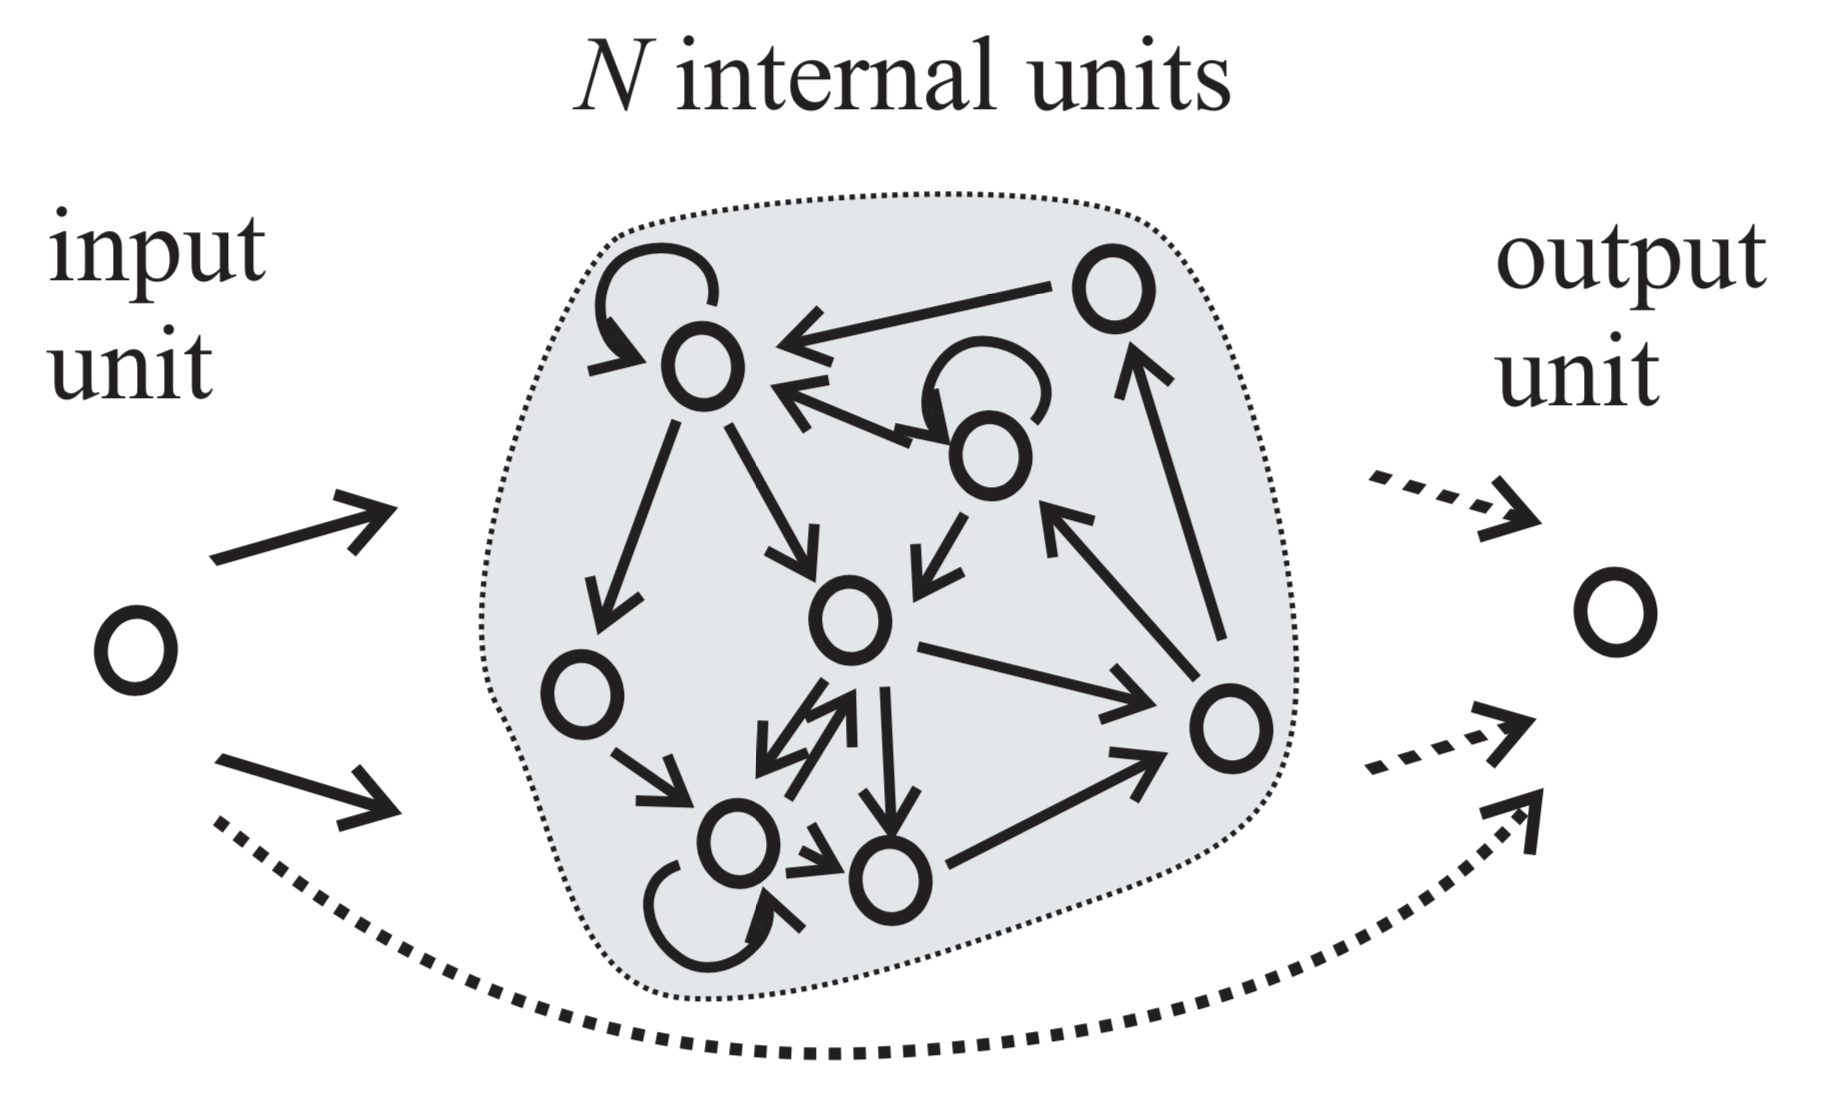
\includegraphics[width=0.7\textwidth]{Pictures/BasicESNStructure.png}
    \end{center}
    \label{FIG:ESNArchitecture}
    \caption{The basic structure of an ESN. Figure taken from \cite{Jaeger2003}. Dotted lines represent trainable connections, whereas solid arrows are fixed connections.}
\end{figure}

Most of the time, the network is being adapted to a specific time series and is trained to perform 1-step ahead predictions, so $u = By$\footnote{B is the backshift operator is defined as $B: \left(\R^n\right)^{\Z} \to \left(\R^n\right)^{\Z}$, $\left(z_t\right)_{t\in\Z} \mapsto \left(z_{t-1}\right)_{t\in\Z}$.}.

Other versions of the basic model can include feedback connections from the output back to the reservoir or the application of leaky-integrator neurons \citep{JAEGER2007335}.
For $\alpha \in \left[0, 1\right]$ and $\wfb \in \R^{N\times L}$ the dynamics of the system \refp{EQ:ReservoirUpdate} accordingly change to
\begin{eqnarray}
    \tilde \bx_t & = & W\bx_{t-1} + \win u_t +  \bb + \wfb y_{t-1} \label{EQ:UpdateLeakyIntegrator}\\
    \bx_t & = & f\left(\alpha \bx_{t-1} + (1-\alpha) \tilde \bx_t \right) \\
    y_t & = & \bx_t \wout  \label{EQ:ESNOutput}
\end{eqnarray}
The leak parameter $\alpha$ can be interpreted as a parametrical way of keeping information within the reservoir nodes. For example, a value of $\alpha = 0.2$ would make the neuron keep $20\%$ of its current information and only allow the newly arriving value of $\tilde x(t)$ to complement this value with a weight of $80\%$. Leaky-integrator neurons would theoretically be possible for the remainder of this thesis but have not been used.

Feedback connections pose a challenge to the training of an Echo State Network because the output connections $\wout$ have to be solved iteratively (because of the need for an output value $y_{t-1}$ in the update \ref{EQ:UpdateLeakyIntegrator}). This could be achieved by an online learning approach (see section \ref{CH:LinearRegression:Online}). However, if the input is chosen as $u = By$ to produce one-step-ahead forecasts of $y$, the target output $y_t$ is the new input to the network by design.

\subsection{Training}

In order to map the network state to a desired output, $\wout$ in \refp{EQ:ESNOutput} can be trained using a linear regression model from section \ref{CH:LinearRegression}.
Hence, the network is being fed the input signal and activations $x_t$ are gathered in a matrix $\tilde X = \left[\bx_0'; \bx_1'; ...; \bx_T'\right] \in \R^{T\times N}$. This regressor matrix can be further enhanced by the addition of an intercept or by the the network input $u$ so that $X = \left(1_{N}, u, \tilde X\right) \in \R^{T\times(2+N)}$.
One could also employ more sophisticated (machine learning) models to map the network activations and the desired output. However, the Echo State Network convinces by its simple and fast training. Additionally, the theory of (high dimensional) linear regression has been studied extensively.

In the training of $\wout$ one has to keep in mind, that the network state has been initialized with $\bx_0 = {\bf 0} \in \R^{N}$. To wash out the effect of the initial state and to prevent misleading training results, an initial transient $\tau$ of observations has to be dropped. The echo state property which will be introduced in section \ref{CH:ESN:ESP} will guarantee, that the effect of (any) initialization fades after several updates of the network. 
This transient can be chosen as a fixed number, or - depending on the size of the dataset - can be set to a fraction of the whole dataset, i.e. $\tau = 0.05\cdot T$. The regressor matrix is truncated accordingly.


\subsection{Hyperparameters}
\label{CH:ESN:Hyperparameters}

Training of Echo State Networks is simple and fast. Most of the connections within the network are initialized randomly and will not be trained to adapt the system to a given task. However, the initialization of those connections has  - as almost all machine learning models do - some hyperparameters that need to be chosen in advance. The choice of (some of) these parameters plays a crucial role in the performance of the model and therefore need special attention. Analytic derivations of optimal parameters are very difficult because of the dynamic and iterative nature of the reservoir. For some there is no analytical solution and other methods such as basic grid search, particle swarm optimization \citep{basterrech2015experimental} or gradient descent \citep{JAEGER2007335} have to be employed. This weighs heavily on the training of time of Echo State Networks. On the other hand, this is also the case for other machine learning models. In the following, we want to present the hyperparameters that are specific to Echo State Networks and come as a tradeoff for not having to train internal connections. % TODO February 29, 2020 : add more
We will go into more detail on the methodology of choosing hyperparameters in section \ref{CH:Application:Methodology}.


\subsubsection{Underyling Probability Distribution of Connections}

In order to initialize the fixed connections within the dynamical system (i.e. $\win$, $W$, $b$), one has to choose some probability distribution\footnote{Typically, the same distribution is chosen for all random initializations.}. Typical choices include the discrete bi-valued\footnote{The discrete bi-valued distribution of weights has a positive chance of creating identical neurons but makes analysis of the reservoir dynamics much easier.} $\mathcal{U}\left\{-1, 1\right\}$, the uniform $\mathcal{U}(-1, 1)$ or the normal distribution $\mathcal{N}(0, \sigma^2)$ for some $\sigma >0$. Even though, \cite{Wu2018StatChallenges} show that the choice of the distribution has an effect on performance, the probability distribution as a hyperparameter doesn't receive much attention and researchers rarely shed any light on their specific choice. Other sources state, that different distributions give almost the same performance because the other hyperparameters are of much higher importance \citep{Lukosecicius2012}. After all, it is worth noting that the distribution of internal weights bears some freedom of choice and may possibly be worth exploring for some tasks.

\subsubsection{Sparsity}

Sparsity is referring to the number of non-zero elements in the internal connections $W$. \cite{Jaeger2004Harness} use a 1\% connectivity to establish a richly structured reservoir of excitable dynamics. Apart from the richness of the reservoir, the computational cost of updating the reservoir is significantly reduced when the connectivity is chosen in relation to the number of total connections. By choosing the sparsity as a fraction of total connections by $s = 10/N^2$ the cost of updating the network only grows linearly with the size of the reservoir instead of quadratically.

\subsubsection{Spectral Radius}

The spectral radius of the internal connections $W$ is the most important hyperparameter for the Echo State Network as it is mainly responsible for the echo state property and the memory capacity of the reservoir. The larger the spectral radius, the more dominant is the echo state (the first part of the update \ref{EQ:ReservoirUpdate}) of the reservoir compared to the new input. So a higher spectral radius means that the reservoir has longer memory and a smaller spectral radius renders the reservoir predominantly a respresentation of the most recent input \citep{Lukosecicius2012}. Depending on the task at hand, one can use some intuituion on the range of plausible spectral radii.


\subsection{Echo State Property}
\label{CH:ESN:ESP}

The echo state property (ESP) is a necessary condition for the network to be able to produce exploitable patterns. Loosely speaking, the echo state property states that the network state is asymptotically independent of its initial state \citep{Jaeger2003}. In other words, the network will forget its initial state and will only depend on a finite set of inputs $u_t$ from a compact set and will forget its initialization, typically ${\bf 0} \in R^{N}$.
The literature offers different approaches to ensure the echo state property. Orginially, \cite{Jaeger2001} stated that choosing the internal connections $W$ such that the spectral radius $\rho(W) = \max \left\{\lambda \,:\, \lambda \text{ eigenvalue of} W\right\}$ is less than unity, would ensure the echo state property for all inputs $u$. This lead to a widespread misconception that the spectral radius always \textit{has} to be smaller than unity. However, depending on the input, larger spectral radii can also be possible without counteracting the echo state property \citep{YILDIZ20121}. \cite{YILDIZ20121} also propose to look at the spectral radius of the corresponding positive matrix $\rho(\abs{W})$ and to ensure that its spectral radius is less than unity. \cite{Ozturk2007AnalysisDesign} propose a procedure to maximize the average state entropy by a spectrum of eigenvalues in the complex plane. \cite{Strauss2012Design} state that the echo state property should be based on the singular values of the connections $W$ instead of its spectral radius. They propose to choose the singular values to be smaller than $1$ to ensure the echo state property. Additionally, the activation function has to be Lipschitz continuous with constant 1\footnote{Which is the case for $tanh$.}. They obtain a sparse and orthogonal matrix $W$ whose singular values and eigenvalues are known to ensure the echo state property.
As there is now direct way to ensure the echo state property for a given input sequence, and some of the above restrictions limiting the performance of the network, the choice of hyperparameters and ensuring for the echo state property falls back to a try-and-error methodology. It is desirable to bring the network dynamics towards the \textit{edge of chaos}, which means to push the dynamics close towards the border between a stable and an unstable regime \citep{LengensteinMaass2007EdgeOfChaos, Buesing2010} to improve computational outcome. 

The choice of the hyperparameters, especially the spectral radius, motivates the following section which targets the tuning of the reservoir beyond its random initialization.


\subsection{Tuning of the Reservoir Dynamics}
\label{CH:ESN:Tuning}

The motivation for the inclusion of this section stems from the nature of another reservoir computing model, namely the State Affine Systems \citep{Grigortega2018SAS}, which changes its dynamics given newly presented input. An Echo State Network is indeed dynamical system, however, the connections within the network are fixed and don't change. They can be interpreted as a restricted and slightly modified State Affine System, where its dynamics, namely $W$ or $\win$, are functions of the input.
This motivated the search for ways to modify the Echo State Network to react differently to different inputs, adapt its dynamics or in general to further improve the reservoir after initialization.

Different endeavours have been undertaken to tune the reservoir beyond the random initialization and the selection of hyperparameters. As mentioned earlier, the most import hyperparameter is the spectral radius\footnote{Other hyperparameters are important as well, but the spectral radius has the largest effect on the performance of the network.}.
\cite{Triesch2005} uses an unsupervised intrinsic learning approach to change the neurons excitability beyond the its random intialization. Using a continuous activation model, he tries to bring the output of each neuron as close as possible to an exponential distribution. 

In order to tune the neuron's output, he transforms the original activation function $f: \R \to \R$, $\bx \mapsto \frac{1}{1+\exp{-\bx}}$ (fermi activation function) using
\begin{equation}
    f_{y}(y) = f(\balpha\odot \bx + \bbeta)
\end{equation}
with tunable parameters $\balpha, \bbeta  \in \R^{N}$. To match the notation of \cite{Triesch2005} and \cite{Schrauwen2008}, $y$ in this instance is not be confused with the network output but represents the post-activation network state. We use vector notations for $\bx, \balpha$ and $\bbeta$ as each element of $\balpha$ and $\bbeta$ is related to a neuron in the network. The modified network update not only tunes the spectral radius but also incorporates the bias $\bb$. The effective update of the network then becomes
\begin{equation}
    \bx_t = f\left(\diag{\balpha}W\bx_{t-1} + \diag{\balpha}\win u_t + \balpha \odot \bb + \bbeta\right)
\end{equation}

Using a gradient descent method, he minimizes the Kullback-Leibler divergence of the transformed output $y$ and the desired output distribution. 
\begin{eqnarray}
    D_{KL} \left(f_y \,\vert\vert\, f_{exp}\right) & = & \int f_y(y) \, \log{\frac{f_y(y)}{\frac{1}{\mu} \exp{\frac{-y}{\mu}}}} \dd y\\
    & = & \int f_y(y) \, \log{f_y(y)} \dd y - \int f_y(y) \, \left(-\frac{y}{\mu} - \log{\mu}\right) \dd y \\
    & = & -H(y) + \frac{1}{\mu} \E{y} +  \log{\mu}
\end{eqnarray}
Where $H(y)$ is the entropy of $y$, and $\E{\cdot}$ is the expectation. In other words, he tries to make the output $y$ be as close as possible to $\frac{1}{\mu} \exp{-y/\mu}$. The last term $\log{\mu}$ is constant and the second term $\frac{1}{\mu}\E{y}$ is equal to $1$ if $y$ follows an exponential distribution with parameter $\mu$. This shows, that the exponential distribution is the maximum entropy distribution \citep{Triesch2005}. Therefore the Kullback-Leibler divergence is minimized, when the entropy is maximized\footnote{This implies the direct connection of the fermi activation function and the exponential distribution.}. Using the gradient with respect to $\balpha$ and $\bbeta$, he comes up with the following stochastic gradient descent rule for $\balpha := \balpha + \Delta\balpha$ and $\bbeta := \bbeta + \Delta\bbeta$ with
\begin{eqnarray}
    \Delta\bbeta & = & \eta \left(1 - \left(2+ \frac{1}{\mu}\right)y + \frac{1}{\mu}y^2 \right) \\
    \Delta\balpha & = & \eta \left(\frac{1}{\balpha} + x - \left(2+ \frac{1}{\mu}\right)\bx y + \frac{1}{\mu}\bx y^2\right) \\
    & = & \frac{\eta}{\balpha} + \Delta\bbeta x
\end{eqnarray}
where $0 < \eta < 1$ is a small learning rate. % TODO February 29, 2020 : much less sign


Different extensions of \cite{Triesch2005} have been proposed, including \cite{Boedecker2009SelfOrganized} who match the neurons' output to a Laplace distribution. Another extension is provided by \cite{Schrauwen2008} who target a gaussian output distribution $\mathcal{N}\left(\mu, \sigma^2\right)$ using the hyperbolic tangent as activation function which is the maximum entropy with support $\left[-\infty, \infty\right]$. They follow the argumentation along the lines of \cite{Triesch2005} and come up with similar updates of the parameters $\balpha$ and $\bbeta$, namely\footnote{They use an equivalent notation for \refp{SchrauwenUpdate1}: $\Delta\beta = - \eta \left(-\frac{\mu}{\sigma^2} + \frac{\by}{\sigma^2}\left(2\sigma^2 + 1 - \by^2 + \mu \by\right)\right)$.}:

\begin{eqnarray}
    \Delta \bbeta & = & -\eta \left(2y + \frac{1}{\sigma^2} \left(1 - y^2\right)\odot(y-\mu)\right) \label{SchrauwenUpdate1}\\
    \Delta \balpha & = & \frac{\eta}{\balpha} + \Delta\bbeta \odot \bx \label{SchrauwenUpdate2}
\end{eqnarray}

\citep{Schrauwen2008} recognize, that the boundedness of the activation function influences the output distribution of the neurons and in turn imposes a certain constraint on the moments of the infinite normal distribution. They analyse the behaviour of their online update and the resulting empirical distributions and find that for certain choices of $\mu$ and $\sigma$ the boundedness significantly truncates the distribution. However, this problem can be easily solved by introducing another transformation of the activation function which is one of the contributions of this thesis. Given $c > 0$ we transform the activation function
\begin{equation}
    f_y(y) = c \cdot \tanh{\frac{\balpha \odot \bx + \bbeta}{c}}
\end{equation}
such that the activation functions maps to the interval $[-c, c]$. Choosing $c$ depending on the parameters of the normal distribution, i.e. the $99.5\%$ quantile or any arbitrary value larger than that, the probability mass that is being truncated by the activation function can be chosen arbitrarily small. The online learning rule for $\alpha$ and $\beta$ straightforwardly becomes:
\begin{eqnarray}
    \Delta \bbeta & = & -\eta \left( \frac{2y}{c^2} + \frac{1}{\sigma^2} \left(1 - \frac{\by^2}{c^2}\right)(\by-\mu)\right) \\
    \Delta \balpha & = & \frac{\eta}{\alpha} + \Delta \beta \bx
\end{eqnarray}
which is equivalent to \refp{SchrauwenUpdate1}-\refp{SchrauwenUpdate2} for $c = 1$. This enables us to choose any value of $\sigma > 0$\footnote{Other activation functions like the $arcsinh$ \citep{KIM2001ARCSINHActivation} or a rectified natural logarithm \citep{Liu2019NaturalLogarithmRectifiedAF} have been considered to achieve the goal of variable boundedness of the activation function but given the solution presented above, have not been further explored.}. The choice of $\mu$ is still limited but can be neglected. This is because network activations centered around $0$ or centered around $\mu \neq 0$ provide the same information and the linear readout can take care of any necessary shift. Figure \ref{FIG:IPTuning} presents the effect of the adaptation of the reservoir towards a target output distribution. The fit is clearly improved and the introduction of the scaling parameter $c$ is justified as we find activation values outside $\left[-1, 1\right]$.


\begin{figure}
    \begin{center}
    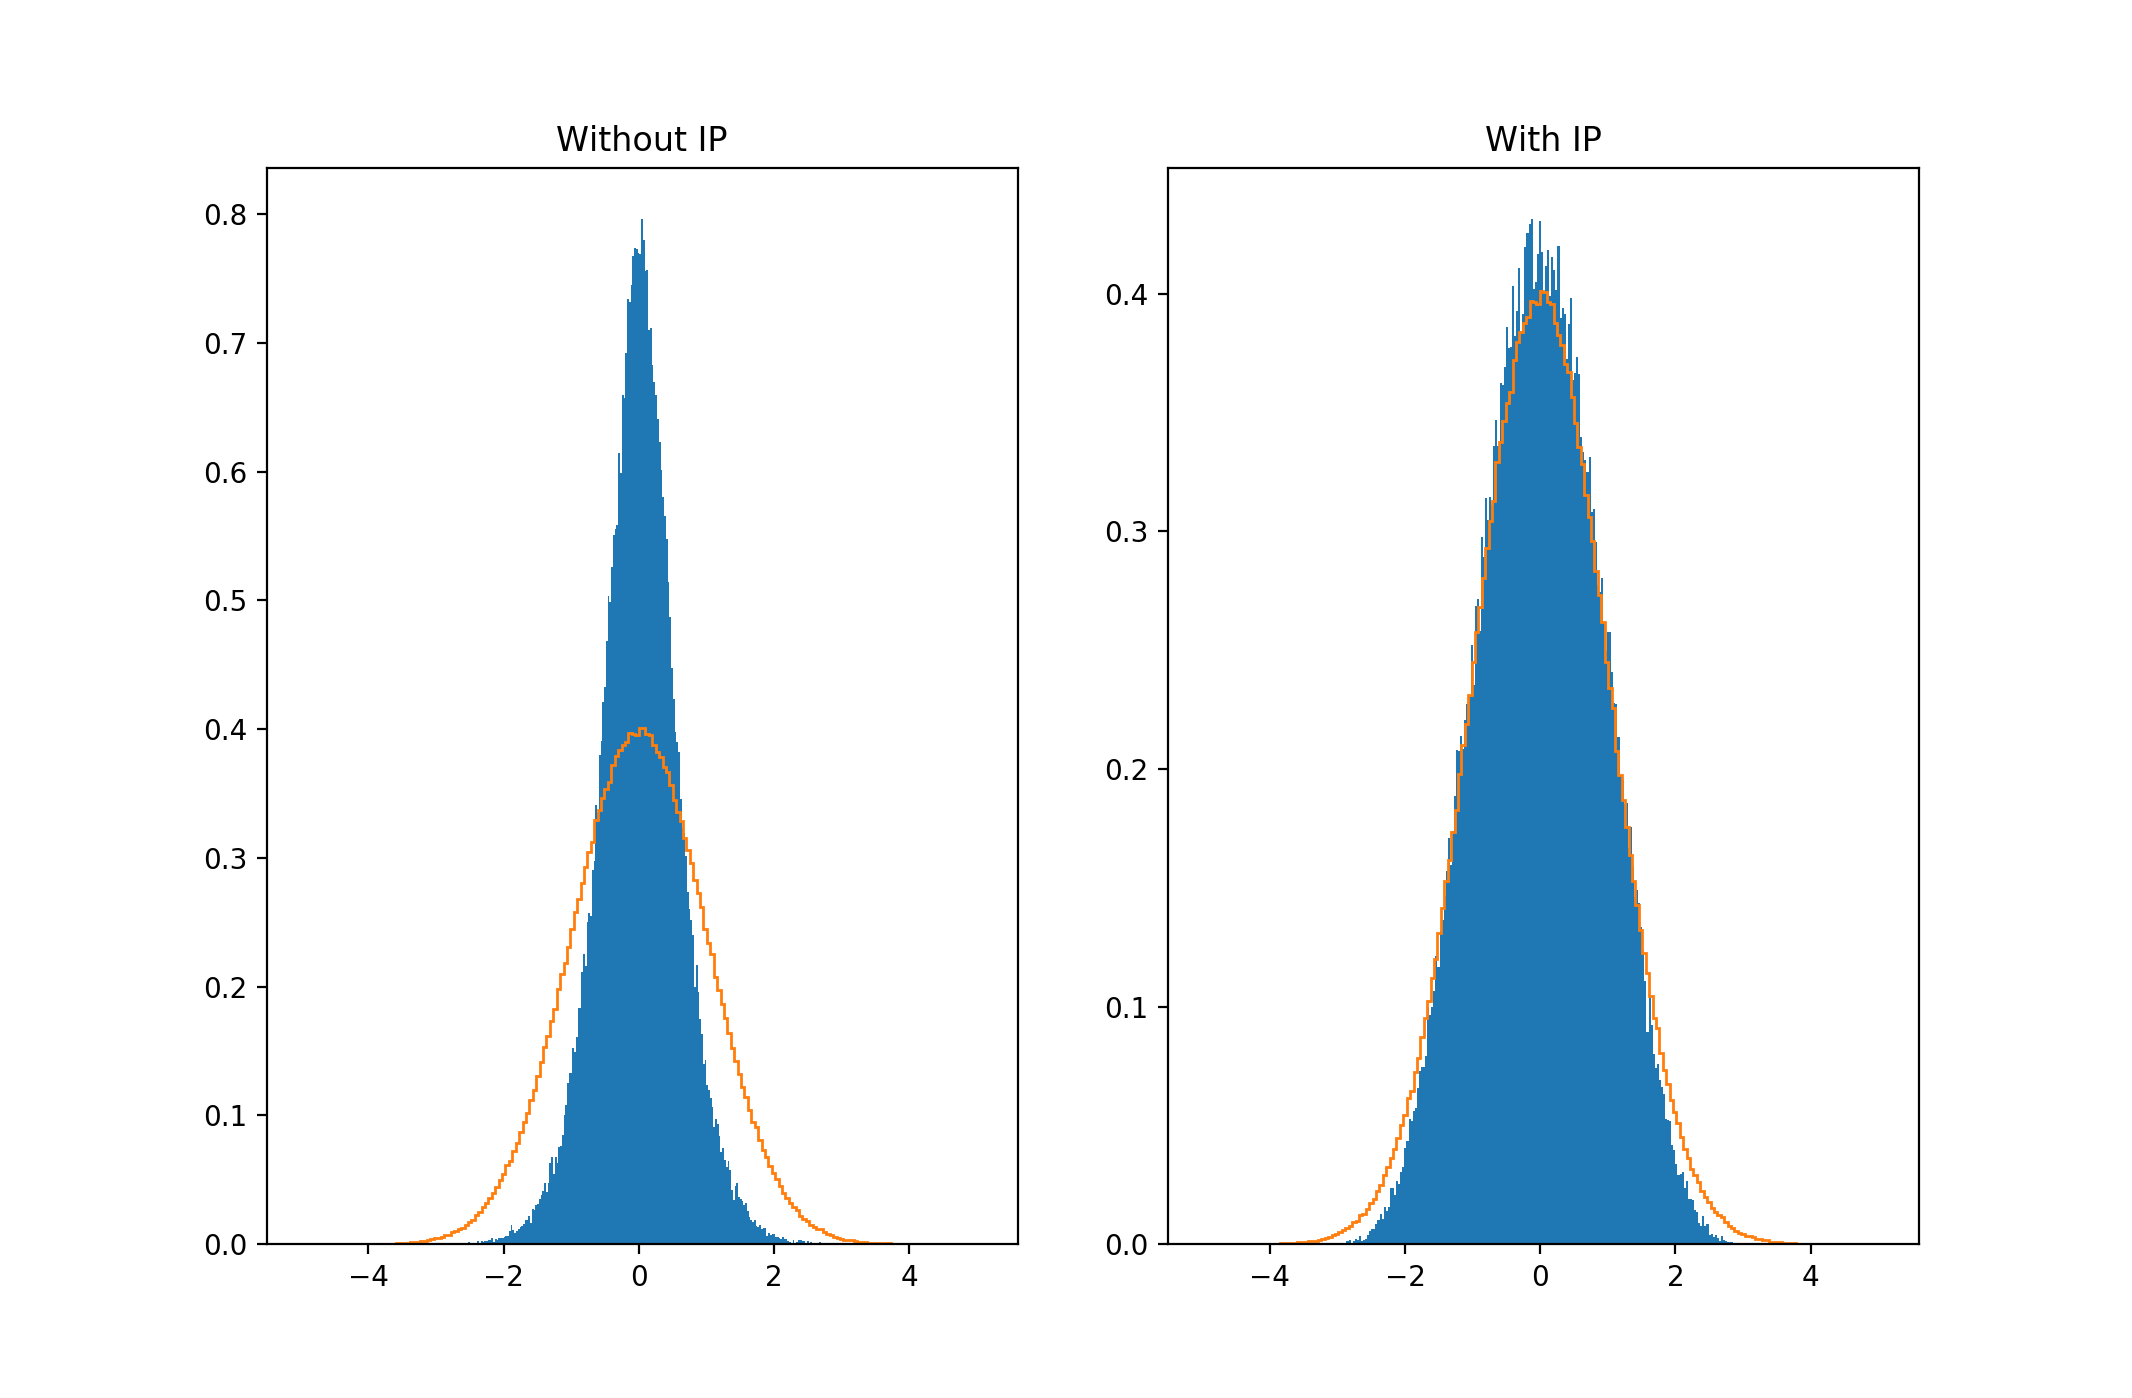
\includegraphics[width=0.9\textwidth]{Plots/IP_KLTANH_sigma1.png}
    \end{center}
    \label{FIG:IPTuning}
    \caption{Network activations of a standard Echo State Network of size $N=1000$ with initial spectral radius of $\rho = 0.95$. Its activation function, as can be seen by the range of activation values, has been adjusted to allow for a wider range of values. The fit of the last $100$ network activations is clearly improved by the transformation. Additionally, the activation values are larger than $1$ which supports the additional of the scaling parameter $c$. Adaptation of the reservoir has been performed for $100$ epochs feeding the Mackey-Glass timeseries of length $5000$ and the scaling of the activation function was chosen as $c=5$.}
\end{figure}

Furthermore, \cite{Koprinkova2011IPandStability} show that the pre-training of an Echo State Network using intrinsic plasticity improves the network stability. They find a close relationship between IP pre-training and stabilization of the reservoir dynamics, such that even initially unstable reservoirs become stable by pushing reservoir activations towards the predefined mean $\mu$ of the normal distribution. They derive the Kullback-Leibler divergence as
\begin{equation}
    D_{KL} = - H(y) + \frac{1}{2\sigma^2}\E{\left(y-\mu\right)^2} + \log{\frac{1}{\sigma\sqrt{2\pi}}}
\end{equation}
which shows the compromise between entropy maximization and minimization of the distance between $\mu$ (typically chosen as $0$) and $y$.

\section{Mixtures of Experts Models}
\label{CH:ExpertModels}

Mixture of experts models cover a wide range of mixture models where multiple expert candidates compete for best performance. Consider yourself a forecaster and you have a certain number of experts or candidates for advice around you and you want to combine or mix their advice into one prediction. The mixture components can be modelled by covariates or functions of the individual candidate's performance.
Having its origin in the machine learning literature, they do appear in many guises \citep{gormley2018mixtures}. The main goal is to predict a unknown sequence $y_1, y_2, ... $ of independent and identically distributed outcome variables. Subject to a loss function, a natural forecasting strategy would be to combine the experts' predictions $\hat y_t^{k}$, $t = 1, 2, ...$ in a weighted average to get the aggregate forecaster's predictions $\hat y_1, \hat y_2, ...$, where $k$ is referring to one of the experts, while keeping the \textit{cumulative regret} (or simply \textit{regret}) with respect to each expert small. The performance of each expert is evaluated subject to a loss function $L: \R^2 \to \R_{>0}$, $(\hat y_t, y_t) \mapsto L(\hat y_t, y_t)$ which enables the definition of the regret as \citep{CesaBianchi2006PredictionLearningGames}
\begin{equation}
    R_n^k = \sum_{t=1}^{n} \left(L(\hat y_t, y_t)-L(\hat y_t^{k},y_t)\right) = \hat L_n - L_{k,n} \label{EQ:Regret}
\end{equation}
where $\hat L_n$ is the forecaster's cumulative loss and $L_{k,n}$ is the cumulative loss of expert $k$. Accodingly, the instant regret to expert $k$ can be defined by $r_{k,t} = L(\hat y_t, y_t)-L(\hat y_t^{k},y_t)$. One can interpret this quantity as the regret the forecaster feels for not having listened to the advice of expert $k$ in the prediction of $y_t$. The main motivation for the employment of multiple experts over a single candidate is the expectation that an ensemble outperforms a single expert (\textit{The wisdom of crowds}). In this sense, the regret should vanish for an increasing number $n$ of observations. That is
\begin{equation}
    \frac{1}{n}\left(\hat L_n - \min_{k} L_{k,n}\right) \to 0 
\end{equation}
for $n\to\infty$. The performance and the ensurance of this goal can only be evaluated in hindsight but regret bounds do exist for different algorithms.

Hence, assume we have finite number $K \in \N$ of possible experts or components and a weighting $\bw_t = \left(w_t^1, ..., w_t^K\right) \in \left[0,1\right]^{K}$ ($t=1,2,...$) at time $t$ of those experts such that $\sum_{k=1}^{K} w_t^k = 1$ for all $t$. Each expert $k$ ($k= 1, ... , K)$ produces a forecast, which in its most general form can be described by a density $f_k(\cdot \,|\, \theta_k)$ depending on a parameter $\theta_k(\bx_t)$ which can be based on a set of covariates $\bx_t$ \citep{gormley2018mixtures}. The goal is to sequentially find a good weighting $\bw_t$ of the experts to combine their predictions. On the basis of the experts' predictions, a final prediction is computed as

\begin{equation}
    p(y_t \,|\, \bx_t) = \sum_{k=1}^{K} w_k f_k(y_t \,|\, \theta_k(\bx_t))
\end{equation}

This model, by allowing $\bw_t$ and $\theta_k(\bx_t)$ to vary in different ways, allows for a wide range of applications, one of which we want to highlight in the following section.

One common way to model $\bw_t$ and $\theta_k(x_t)$ is to choose a point forecast $\hat y_t^{k}$ instead of a density $f_k ( y_t \,|\, \theta_k(x_t))$. The forecaster chooses a weighting $\bw_t$ of the experts and combines their individual point forecasts $\hat y_t^{k}$ by
\begin{equation}
    \hat y_t = \sum_{k=1}^{K} \bw_t^{k} \hat y_t^{k}
\end{equation}
and - by observing the true value $y_t$ - suffers a non-negative loss $L(\hat y_t, y_t)$. Now the performance of each expert can be judged based on the loss function $L$ or equivalently on each expert's regret $R_n^k$ from \refp{EQ:Regret}.


\subsection{Loss Induced Weighting of Experts}
\label{CH:ExpertModels:Loss}

It seems intuitive to update the weighting of the experts based on their performance, such that an expert with a high regret receives a higher weight because it would have been advisable to 'listen' to him and an expert with a comparably lower regret receives a lower weight. This can be achieved by different approaches \citep{CesaBianchi2006PredictionLearningGames}
\begin{eqnarray}
    \text{Linear:} & w_t^k = & \frac{R_t^k}{\sum_{i=1}^K R_t^{i}} \\
    \text{Polynomial:} & w_t^k = & \frac{2(R_t^k)_{+}^{p-1}}{\left(\sum_{i=1}^K (R_t^{i})^p\right)^{(p-2)/p}} \\
    \text{Exponential:} & w_t^k = & \frac{\exp{\eta R_t^k}}{\sum_{i=1}^{K} \exp{\eta R_t^i}}
\end{eqnarray}
to differently weight the regret where the fractions are needed to normalize the weights to ensure $\sum_{k=1}^{K} w_t^k = 1$. $( \, \cdot \,)_{+}$ is referring to the positive part, so $(x)_{+} = \text{max}\left\{0, x\right\}$. The exponential update introduces a learning rate $\eta > 0$ which bears a drawback of the exponential weighting because of the introduction of a hyperparameter that may be subject to optimization. Nevertheless, we will focus on this approach because of its nice properties and the similarity to the plasticity weighting which we will introduce in section \ref{CH:ExpertModels:Plasticity}. One major advantage of the exponentially weighted approach is the fact that it can be equivalently formulated as an incremental update of the weights by inserting \refp{EQ:Regret}
\begin{eqnarray}
    w_t^k & = & \frac{\exp{\eta R_t^k}}{\sum_{i=1}^{K} \exp{\eta R_t^i}} \\
    & = & \frac{\exp{\eta \sum_{\tau=1}^{t} \left(L(\hat y_\tau, y_\tau)-L(\hat y_\tau^{k},y_\tau)\right)}}{\sum_{i=1}^{K} \exp{\eta \sum_{\tau=1}^{t} \left(L(\hat y_\tau, y_\tau)-L(\hat y_\tau^{i},y_\tau)\right)}} \\
    & = & \frac{w_{t-1}^k\exp{\eta \left(L(\hat y_t, y_t)-L(\hat y_t^{k},y_t)\right)}}{\sum_{i=1}^{K} w_{t-1}^i\exp{\eta \left(L(\hat y_t, y_t)-L(\hat y_t^{i},y_t)\right)}} \\
    & = & \frac{w_{t-1}^k\exp{-\eta L(\hat y_t^{k},y_t)}}{\sum_{i=1}^{K} w_{t-1}^i\exp{-\eta L(\hat y_t^{i},y_t)}} \label{EQ:LossUpdate} 
\end{eqnarray}
This update of weights only requires the last performance of the experts as opposed to the linear or polynomial update that depend on the regret and therefore on past predictions $\hat y_s^k$, for $s < t-1$ and $k = 1, ..., K$. Different choices of $\eta$ can lead to different performance results and one can circumvent its optimization by knowledge of the forecasting horizon which can help to choose $\eta$ in advance.


% Elaborate more on the regret.
One objective of the forecaster is to choose the learning rate of any algorithm for $w_t$ such that the regret is low. \cite{CesaBianchi2006PredictionLearningGames} prove different performance bounds for the weight updates mentioned above. The exponential update for a convex loss function $L: \R^2 \to [0,1]$ is proven to be
\begin{equation}
    \hat L_n - \min_{k=1,...,K} L_{k,T} \leq \frac{\log{K}}{\eta} + \frac{T\eta}{8} \label{EQ:OptimalLearningRate}
\end{equation}
for any $T > 0$ referring to the number of observations and any $\eta > 0$. Minimizing this upper bound with respect to $\eta$ one can choose $\eta = \sqrt{8\log{K}/T}$ which results in the minimal upper bound of $\sqrt{(T/2)\log{K}}$. This procedure, however, requires prior knowledge of the forecasting horizon $T$. If this is not known in advance, \cite{CesaBianchi2006PredictionLearningGames} further propose a time dependent learning rate $\eta_t$ that has a regret bound that holds uniformly over time. By choosing
\begin{equation}
    \eta_t = \sqrt{8\ln{K}/t}
\end{equation}
which comes back to an argument of resetting the optimal learning rate in \refp{EQ:OptimalLearningRate} after every prediction and considering only 1-step ahead prediction horizons, the regret bound becomes ....... % TODO March 16, 2020 : insert regret bound


\subsection{Pre-Prediction Update of Weights}

One of the main drawbacks of the loss induced expert weighting introduced in section \ref{CH:ExpertModels:Loss} is the fact that the weighting of the experts can be adjusted \textit{after} the loss has been suffered, i.e. after the prediction. To our knowledge, no research in this specific setting has been undertaken so far to update the weights of a set of Echo State Networks \textit{prior} to the prediction step. Coming up with measures to judge an expert's expected performance seems difficult but different sources lead to main part of this thesis which tackles this problem.

\subsubsection{Gaussian Mixture Autoregressive Model}
\label{CH:ExpertModels:GMM}

\cite{Kalliovirta2015GMUnivariateSeries} present a Gaussian Mixture Autoregressive Model (GMAR) where they use a particular choice of the mixing weights for a set of $K \in \N$ experts, each of them being an auxiliary, stationary AR(p) process. The stationary solution of such an AR(p) process specifies a mean value and an autocovariance structure on the time series. The mixing of those processes (experts) is based on the likelihood that the last $p$ observations of the target time series have been generated by any of those processes. Set ${\bf y}_{t-1} = \left(y_{t-1},...,y_{†-p}\right) \in \R^{p}$. They use the multivariate normal distribution $\mathcal{N}(\bmu^{k}, \Sigma^{k})$, $\mu^{k} \in \R^{p}$ and $\Sigma^{k} \in \R^{p\times{}p}$ for $k = 1, ..., K$, with density
\begin{equation}
    f^{k}(\by_{t-1}) = \frac{1}{\sqrt{(2\pi)^k \vert \Sigma^{k} \vert}} \text{exp}\left(-\frac{1}{2}\left(\by_{t-1}-\bmu^{k}\right)'(\Sigma^{k})^{-1}\left(\by_{t-1}-\bmu^{k}\right)\right)
\end{equation}
Subject to a mean weight $\balpha = \left(\alpha_1, ..., \alpha_K\right) \in \R^{k}$, they define the mixing weights $\alpha_{k,t}$ as
\begin{equation}
    \alpha_{k,t} = \frac{\alpha_k f^{k}(\by_{t-1})}{\sum_{i=1}^{K} \alpha_i f^{i}(\by_{t-1})}
\end{equation}

This method of weight update is - as within the expert setting - performed before the predition of the next value as one has uses the observations up to $y_{t-1}$ in order to predict $y_t$ which makes the process $\by_t$ Markovian.

\subsubsection{Echo State Incremental Gaussian Mixture Network}
\label{CH:ExpertModels:ESIGMN}

Another, very rich, line of research is \citep{Engel2010IncrementalGaussianMixtures, Heinen2011IGMN, Heinen2011ACA}. In one of their publications, \cite{ESIGM2011} propose a novel algorithm for incremental temporal pattern processing called the Echo State Incremental Gaussian Mixture Network (ESIGMN). It combines Echo State Networks with the Incremental Gaussian Mixture Network (IGMN) from \cite{Heinen2011IGMN}. 

The Incremental Gaussian Mixture Network is composed of multiple sets of virtual neurons (referred to as cortical regions), all of which have size $M \in \N$ and an association region. Figure \refp{FIG:IGMN} from their paper visualizes the model. 

\begin{figure}
    \begin{center}
    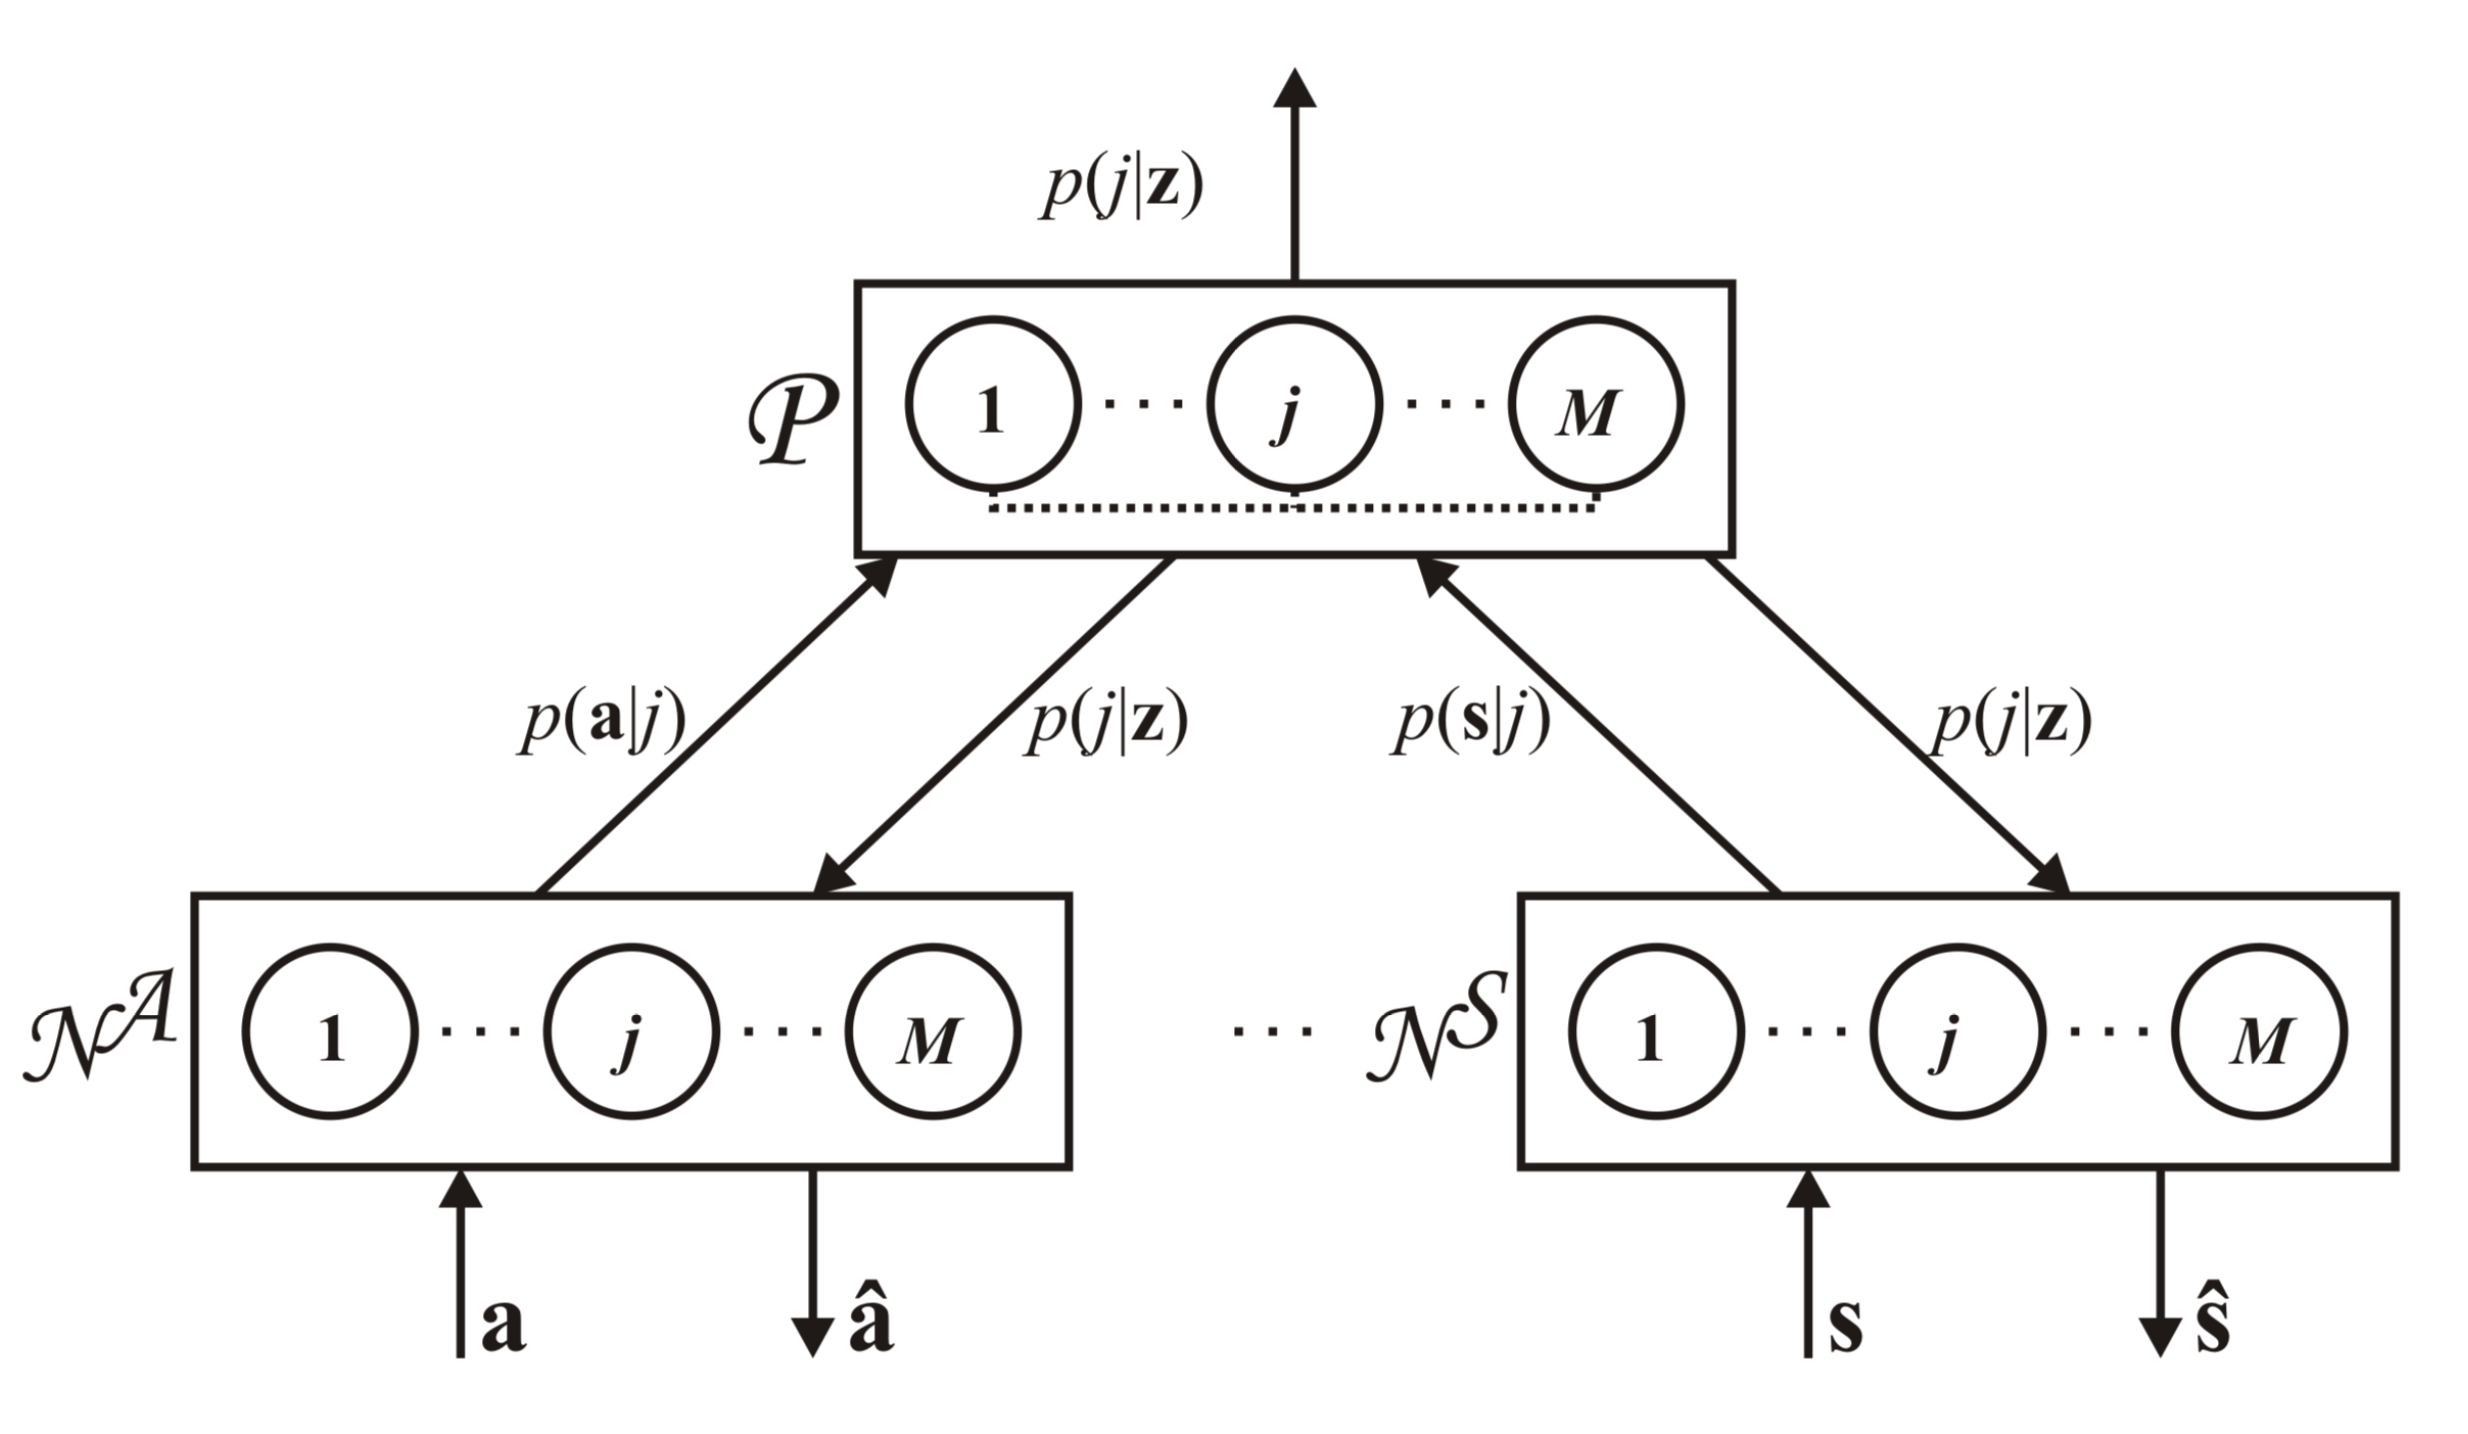
\includegraphics[width=0.7\textwidth]{Pictures/IGMN_Structure.png}
    \end{center}
    \label{FIG:IGMN}
    \caption{Basic architecture of the Incremental Gaussian Mixture Network from \cite{Heinen2011IGMN}. $\mathcal{N}^{\mathcal{A}}$ to $\mathcal{N}^{\mathcal{S}}$ refer to the coritcal regions and $\mathcal{P}$ is the association region. The cortical regions are only connected via the association region. New inputs are denoted by ${\bf a}$-${\bf s}$.}
\end{figure}

The IGMN is a gaussian mixture model with an agressive learning process, meaning the training data only has to be presented once. Based on $K \in \N$ distribution components (these are the \textit{cortical regions}) the network can adapt to the information from a new data point. One can think of the cortical regions as individual neural networks. Presented with a new input $u$\footnote{The notation has been adjusted to match our setting so far.}, a running mean $\mu_k$ and running covariance $\Sigma_k$ of network activations for each network are maintained\footnote{For details on the exact update of $\mu_k$ and $\Sigma_k$, the reader is referred to their paper.}. Based on these, the likelihood of each component $k$ is can be calculated:

\begin{equation}
    p \left(u \, | \, k\right)= \frac{1}{(2\pi)^{M/2}\sqrt{\abs{\Sigma_k}}} \exp{-\frac{1}{2}(u - \mu_k)'\Sigma_k^{-1}(u-\mu_k)}
\end{equation}

where $M$ is the size of component $k$. Given a prior distribution $p(k)$ which is initialized as $p(k) = \frac{1}{K}$ ($k = 1, ..., M$) posterior probabilites can be calculated for each component

\begin{equation}
    p(k \, | \, u) = \frac{p \left(x \, | \, k\right) p(j)}{\sum_{k=1}^{K} p \left(x \, | \, k\right) p(k)} \label{EQ:ESIGMN:posterior}
\end{equation}

The prior distribution $p(k)$ is also updated based on \refp{EQ:ESIGMN:posterior}. The recostruction of a target signal by the network is then produced as a weighted average of the individual regions' predictions 

\begin{equation}
    \hat y = \sum_{k=1}^{K} p(k \, | \, u) \hat y_m
\end{equation}

Where $\hat y_m$ is the prediction of the $m$-th component based on a Gaussian Process Regression. We will refrain from going into more detail, the interested reader is referred to their paper.

The further enhancement of \cite{ESIGM2011} to this idea is the preprocessing of the input $u$ by a single Echo State Network and the application of the Incremental Gaussian Mixture Network after the input has been transformed into a higher-dimensional representation.


\subsubsection{Plasticity based Weighting}
\label{CH:ExpertModels:Plasticity}

Both of the approaches outlined above are working with a likelihood based methodology to weight the predictions of a set of models (experts). As opposed to the loss induced weighting of experts, they choose the likelihood as a measure that is not related to the actual prediction error or loss, that the components suffer indivually. Accordingly, their model designs favour such an approach. 

To transfer this idea of a likelihood based weighting, the combination of \cite{Schrauwen2008}, \cite{Kalliovirta2015GMUnivariateSeries} and \cite{ESIGM2011} inspired a weighting of experts of echo state networks that is updated prior to the prediction step and is not necessarily dependent on a loss function $L$.

Given $K \in \N$ experts, each being an Echo State Network, we define $\bsigma := \left(\sigma_1, ..., \sigma_K\right)$, $\bmu := \left(\mu_1, ..., \mu_K\right) \in \R^{K}$. Assume we have tuned each of the networks by the approach of \cite{Schrauwen2008} with a target normal distribution $\mathcal{N}(\mu_k, \sigma_k^2)$ for $k = 1, ..., K$. Associated to these experts is a weight vector $\bw_t = \left(w_t^{1}, w_t^{2}, ..., w_t^K\right)$ where the index $t$ corresponds to a point in time.
After the network has been presented a new input and has been update to reflect the state $\bx_t$, the update of $\bw_t$ is based on the likelihood. Accordingly, weights are updated in the following way

\begin{eqnarray}
    \tilde w_{t}^{k} & = & p(x_t^k \, | \, \mu_k, \sigma_k^2) \nonumber \\ 
    & = & w_{t-1}^{k} \frac{1}{\sqrt{2\pi\sigma_k^2}} \exp{- \frac{\left(x^{k}_{t} - \mu_k\right)'\left(x^{k}_{t} - \mu_k\right)}{2\sigma_k^2}} \label{EQ:Likelihood}\\
    & & \text{for } k = 1,..., K \nonumber \\
    \bw_t & = & \frac{\tilde \bw_t}{\sum_{k=1}^{K}\tilde w_t^k}
\end{eqnarray}

This makes intuitive sense because the $k$-th Echo State Neworks has been tuned to follow a normal distribution with mean $\mu_k$ and variance $\sigma_k^2$ and, thereby, to achieve an information-maximization. Ranking the networks by their states' likelihood is equivalent to using the Kullback-Leibler divergence that has originally been used to move the network towards the targeted distribution.
As argued in section \ref{CH:ESN:Tuning}, $\mu_k$ can be set to $0$ and $p(\cdot \, | \, \mu, \sigma_k^2)$ refers to the density of a normal distribution with the given parameters\footnote{As will further be elaborated on in section \ref{CH:Application}, numerical accuracy in the calculation of \refp{EQ:Likelihood} can become critical, when the size $N$ of neurons in each expert gets large.}.
Let $N \in \N$ be the number of total neurons aggregated over all experts and $n = \frac{N}{K}$ be the size of one expert, define $\win^k$, $W^k$, $\wout^k$ and $\bb^k$ like in section \ref{CH:ESN:Architecture} and initialize $\bx_0^k = {\bf 0} \in \R^{n}$. We can outline the algorithm for the plasticity weighted experts of Echo State Networks

\begin{eqnarray}
    \bx_{t}^k & = & f\left(W^k\bx_{t-1}^k + \win^k u_t +  \bb^k\right) \\
    \tilde w_{t}^{k} & = & w_{t-1}^{k} \frac{1}{\sqrt{2\pi\sigma_k^2}} \exp{-\frac{\left(\bx^{k}_{t} - \mu_k\right)'\left(\bx^{k}_{t} - \mu_k\right)}{2\sigma_k^2}} \label{EQ:PlasticityWeightUpdate}\\
    & & \text{for } k = 1, ..., K \nonumber \\
    \bw_t & = & \frac{\tilde \bw_t}{\sum_{k=1}^{K}\tilde w_t^k} \\
    \hat y_t & = & \sum_{k=1}^K w_t^k \bx_{t}^k\wout^k \label{EQ:PlasticityPrediction}
\end{eqnarray}

For the ease of notation, the addition of an intercept or the input $u_t$ into \refp{EQ:PlasticityPrediction} has been neglected but surely is possible.
Combining this with an online training of the output connections $\wout^k$ (see section \ref{CH:LinearRegression:Online}) can produce a one-shot prediction cycle then can be run and updated perpetually.

\subsubsection{Equivalence of Exponential and Plasticity Weighting}
\label{CH:ExpertModels:Equivalence}
We want to show the equivalence of the loss induced weighting and the proposed plasticity based weighting of experts and try to present the relationship of the two under certain conditions. These assumptions are mostly based on a good adaptation of the reservoir dynamics towards a targeted distribution such that we can infer some statistical features of the network activation which would otherwise not be possible without the pre-training of the reservoir dynamics.
The equivalence of the proposed plasticity approach and the exponential weighting of experts can be shown under the following assumptions:

\begin{enumerate}
    \item The loss function $L$ for the loss induced weighting is chosen to be the \textit{Mean Squared Error} which is $L(x,y) = \left(x - y\right)^2$. \label{Assumption:Loss}
    % \item The input series $u_t$, hence the target output $y_t = Bu_t$, as well as the network activations $x_t^k$ are centered around $0$, e.g. $\E{u_t} = 0$. \label{Assumption:Centered}
    \item The output model doesn't include an intercept or the input $u$. This means, the output of the model is exclusively based on the activation values of the network's neurons. \label{Assumption:OutputModel}
\end{enumerate}

Using assumption \refp{Assumption:Loss} the update of weights for the loss induced weighting \refp{EQ:LossUpdate} and the plasticity \refp{EQ:Likelihood} approach already look similar:

\begin{eqnarray}
    \tilde w_t^k & = & \tilde w_{t-1}^{k}\exp{-\eta \left(\hat y_t - y_t\right)^2} \label{EQ:ExpertUpdateMSE}\\
    \hat \bw_t^k & = & \hat w_{t-1}^{k} \frac{1}{\sqrt{2\pi\sigma_k^2}} \exp{-\frac{\left(\bx^{k}_{t} - \mu_k\right)'\left(\bx^{k}_{t} - \mu_k\right)}{2\sigma_k^2}}
\end{eqnarray}

where $\tilde w$ and $\hat w$ refer to the expert and the plasticity approach, respectively. Choosing $\eta > 0$ separately for each expert $k$ as $\eta_k = \frac{1}{2\sigma_k^2}$ and targeting all of the neuron's output to $\mu_k = 0$ for all $k$, the argument of the exponential function is aligned and the plasticity update becomes

\begin{equation}
    \hat w_t^k = \hat w_{t-1}^{k} \frac{1}{\sqrt{\pi\eta_k}} \exp{-\eta_k\left(\bx^{k}_{t}\right)^2}
\end{equation}

where $\left(\bx^{k}_{t}\right)^2 =\bx^{k}_t\left(\bx^{k}_t\right)'$ is the inner product of $\bx^k_t$. In order to finally compare the two approaches, one has to take the stance of a pre-prediction update of the loss induced weighting by the expected error.
\cite{Kerridge1967ErrorsOfPrediction} argues that

\begin{equation}
    \hat y_t^k - y_t  = z_k\sigma_{\varepsilon_k} \left[ \left(\bx_t^k - \bar \bx^k\right)' S_k^{-1} \left(\bx_t^k - \bar \bx^k\right) + 1 + \frac{1}{n} \right]^{1/2} \label{EQ:ErrorDistribution1}
\end{equation}

where $S_k$ is the sample covariance of network activations, a bar denotes the average of past network activations, $\sigma_{\varepsilon_k}$ is the prediction error of the linear model corresponding to expert $k$ and $z_k \sim \mathcal{N}(0,1)$ for $k = 1, ..., K$, all up to time $t-1$. Under ideal conditions, we add the following assumptions:

\begin{enumerate}
    \setcounter{enumi}{2}
    \item $\bar \bx^k = 0$ because we have tuned the network activations to follow a normal distribution with mean $0$. \label{Assumption:Mean}
    \item $S_k = \sigma_k^2 1_n$ is a diagonal matrix with $\sigma_k^2$ on its diagonal. \label{Assumption:Diag}
\end{enumerate}
Both of these assumptions are in line with the methodology of the plasticity weighting. Therefore, \refp{EQ:ErrorDistribution} simplifies to

\begin{equation}
    \hat y_t^k - y_t  = z_k\sigma_{\varepsilon_k} \left[ \frac{1}{\sigma_k^{2}}\left(\bx_t^k\right)^2 + 1 + \frac{1}{n} \right]^{1/2} \label{EQ:ErrorDistribution2}
\end{equation}

which implies

\begin{equation}
    \left(\hat y_t^k - y_t\right)^2  = z_k^2\sigma_{\varepsilon_k}^2 \left[ \frac{1}{\sigma_k^{2}}\left(\bx_t^k\right)^2 + 1 + \frac{1}{n} \right]\label{EQ:ErrorDistribution3}
\end{equation}

Finally, we can conclude

\begin{eqnarray}
    \E{\left(\hat y_t^k - y_t\right)^2} & = & \E{z_k^2}\sigma_{\varepsilon_k}^2 \left[ \frac{1}{\sigma_k^{2}}\left(\bx_t^k\right)^2 + 1 + \frac{1}{n} \right]\label{EQ:ErrorDistribution4} \\
    & = & \sigma_{\varepsilon_k}^2 \left[ \frac{1}{\sigma_k^{2}}\left(\bx_t^k\right)^2 + 1 + \frac{1}{n} \right]\label{EQ:ErrorDistribution4} \\
    & = & \frac{\sigma_{\varepsilon_k}^2 }{\sigma_k^{2}}\left(\bx_t^k\right)^2 + \sigma_{\varepsilon_k}^2\left(1 + \frac{1}{n} \right)\label{EQ:ErrorDistribution5} 
\end{eqnarray}

because $z_k^2 \sim \chi^2_1$ and $\E{z_k^2} = 1$. So we find a direct relationship between the expected loss $\E{\left(\hat y_t^k - y_t\right)^2}$ and the network activation $\bx_t^k$.

Substituting the loss in \refp{EQ:ExpertUpdateMSE} for its expected value, and using \refp{EQ:ErrorDistribution5} yields
\begin{eqnarray}
    \tilde w_t^k & = & \tilde w_{t-1}^{k}\exp{-\eta \E{\left(\hat y_t^k - y_t\right)^2}} \\
    & = & \tilde w_{t-1}^{k} \exp{-\eta \left( \frac{\sigma_{\varepsilon_k}^2}{\sigma_k^{2}} \left(\bx_t^k\right)^2 + \sigma_{\varepsilon_k}^2\left(1 + \frac{1}{n} \right) \right) } \\
    & = & \tilde w_{t-1}^{k} \exp{-\eta        \frac{\sigma_{\varepsilon_k}^2}{\sigma_k^{2}} \left(\bx_t^k\right)^2 } \underbrace{\exp{-\eta \sigma_{\varepsilon_k}^2\left(1 + \frac{1}{n} \right)}}_{=: \zeta} \label{EQ:ExpertVSPlasticity}
\end{eqnarray}
with a constant factor $\zeta$ that doesn't influence the effective weighting. So the updates of weights can be regarded as equivalent up to some difference in the learning rate. Even this difference can be overcome by choosing $\eta$ of the experts approach appropriately as $\eta = \frac{\sigma_{\varepsilon_k}^2}{2}$ for the equivalence of \refp{EQ:PlasticityWeightUpdate} and \refp{EQ:ExpertVSPlasticity} up to some constant factor.



% \section{Framework}
\label{CH:Framework}



In this section we are going to present the empirical setup for the training and performance evaluation using two different time series. On the one hand, we are going to look at the Mackey Glass chaotic time series, which is often considered when looking at time series predictions. It is a time-delay differential equation that exhibits chaotic behaviour which can be tuned by different parameters (see section \ref{CH:EmpiricalResults}). On the other hand, we are going to employ our model on real world financial data, namely the stock price evolution of IBM, which we will try to predict on different frequencies.\\ 
As already mentioned in section \ref{CH:Model}, the training of the network consists of two steps, namely the tuning of hyperparameters and the training of a (linear) model for the hidden-to-output connections.

\subsection{Methodology}

In order to make forecasts of time series, we will run the network and gather its network activations. With the full regressor matrix $X$ we will then employ a the linear model. For our application we chose a leaky integrator ESN with bias. The linear models will be simple linear regression for the Mackey-Glass time series and Logistic Regression as well as Ridge Regression with cross validation for the IBM stock price. Hyperparameters will be tuned on the given training set and will be kept constant for the whole forecasting window, where predictions will only be made one step ahead.


\subsection{Training}
As mentioned in section \ref{CH:Intro}, we consider matrix representations of input, reservoir states and output series. For example the input series is $u \in \R^{T\times K}$ and accordingly $u(t) \in \R^{1\times K}$ with length $T\in\N$ and $K\in\N$ inputs.
Training of an Echo State Network can be summarized in a few steps. 
\begin{enumerate}
\item Select hyperparameters of the chosen architecture and initialize the random connections accordingly. Initialize the reservoir state by $x(0) = \bf{0} \in \R^{N}$.
\item Feed the network with the feature signal $u$ and update the network states according to the chosen architecture. Gather the network activations into a matrix $\tilde X \in \R^{T\times N}$ where $T\in \N$ is the length of the feature series.
\item Drop a specified number $b \in \N$, $b < T$, of first observations of $\tilde X$, as well as in $u$ and $y$ to wash out the influence of the 0-initialization of the reservoir state and concatenate the input and the reservoir states $X = \left[u; \tilde X\right] \in \R^{(T-b)\times(K+N)}$. The inclusion of an intercept depends on the task and can be part of the regressor matrix $X$.
\item Employ a (linear) model $y = X\beta + \eps$ and measure its performance.
\end{enumerate}
Depending on the size of the network one has to employ some regularization in order to get decent forecasting performance. Often times ridge regression is employed, but depending on the nature of the time series that will be forecasted, one may also choose different models. In section \ref{CH:EmpiricalResults}, we will shed some light on why regularization is not necessary for non-stochastic time series like the Mackey-Glass.


The choice of hyperparameters forms the first step of this training procedure and their optimization poses a difficult task. Given the random initialization of the reservoir, analytical solutions have not been found so far and efficient optimization is still under research. Often times, basic grid search is employed. With the original main focus on the internal connections $W$ and the spectral radius, the admissible space for this hyperparameter is unbounded (keeping in mind, that $\rho(W) > 1$ doesn't necessarily destroy the ESP). The choice of the spectral radius in conjunction with the stability of the network depends on the input has to examined by try and error. By switching to the spectral radius of the corresponding positive matrix $\abs{W} = \left(\abs{w_{ij}}\right)$ (see section \ref{CH:Model:SpectralRadius} and \citep{YILDIZ20121}), this problem would be remedied by choosing $\rho$ from the bounded interval $(0,1)$. However, this may be too restrictive for some tasks. We will go with the original definition of the spectral radius.

What really makes life easier in terms of hyperparameter optimization is the fact, that properties of smaller reservoirs regarding their memory and general capabilities, often translate onto larger reservoirs and therefore, optimization can be performed with relatively small reservoirs.\footnote{There is a minimum size for the reservoir to function properly, see \citep{Lukosecicius2012}.} Afterwards, one can increase the size and repeat the training steps to get a powerful and well tuned model.

In our setting we will use the Python package {\it scikit-optimize} for the optimization of hyperparameters, which is a powerful library to minimize (very) expensive and noisy black-box functions\footnote{Homepage with useful examples as well as theory: \url{https://scikit-optimize.github.io}. More details are provided in Appendix \ref{A:ScikitOptimize}}.





\section{Application}
\label{CH:Application}

The statistical characteristics of financial asset returns play a crucial role in today's economy. Risk assessment has become ever increasingly important given not only the recent history of financial markets\footnote{US-China trade war, corona virus outbreak, ...}. The financial crisis of 2007/2008, the burst of the 'dot com' bubble in the year 2000 and many other examples have shown that the financial market can cause major distress in banks, companies and for individual investors. The modeling of the first moment of the return distribution is important but for risk assessment, the most critical feature of the return distribution is its second moment, the variance, which has spurred a wide literature on forecasting and modeling of asset return characteristics. The following builds the foundation for the application of our model(s) to real world data.



\subsection{Mathematical Foundations}

The return process of a financial asset can be discribed by 
\begin{equation}
    r_{t+h} = P_{t+h} - P_t = \log{\tilde P_{t+h}} - \log{\tilde P_t}
\end{equation}
where $\tilde P_t$ is the price process of the asset. In the seminal work of \cite{Andersen2001DistributionofVola} and \cite{Andersen2003ModelForecastVola} they define the one-dimensional stochastic (Itô) process
\begin{equation}
    P_{t+h} - P_t = \int_{t}^{t+h} \mu_s \dd s + \int_{t}^{t+h} \sigma_s \dd B_s
\end{equation}

with a standard Brownian motion $B_t$, $\mu_s$ is a locally bounded and predictable dift process and $\sigma_s$ is the right-continuous and left-limit volatility. Given a sequence of partitions $\left(D_m\right)_{m\in\N}$ with $D_m = \left\{0 = t_1 < ... < t_m = T\right\}$ with $\sup_{1 \leq i \leq m} \abs{t_i - t_{i-1}} \to 0$ for $m \to \infty$, the quadratic variation $\langle P\rangle_t$ of $r_{t+h}$ is defined as
\begin{equation}
    \langle P\rangle_t = \lim_{m \to \infty} \sum_{\stackrel{t_i \in D_m}{t_i < t}} \left(P_{\text{min}\left(t_{i+1}, t\right)} - P_{t_i}\right)^2 \label{EQ:QuadraticVariation}
\end{equation}
which exists in probability. \cite{Billingsley2008} shows that
\begin{equation}
    \langle P\rangle_t = \int_{0}^{T} \sigma_s^2 \dd s \label{EQ:IntegratedVariance}
\end{equation}
which is known as integrated variance.

\subsection{Realized Volatility}
\label{CH:Application:RV}

\cite{NielsenShephard2004} were the first to introduce a consistent estimator for the integrated variance \refp{EQ:IntegratedVariance}\footnote{They even propose an estimator for integrated covariance.} under the assumption of no market microstructure noise\footnote{Market microstructure is concerned with the formation of the price and the 'noise' around it which arises from timing of transactions, flow and disclosure of information and the individual behaviour of market participants.}. Given the log-price process introduced earlier, they propose the Realized Volatility\footnote{The original papers were concerned with the Realized Variance but we will denote by $RV$ the Realized Volatility, so the square root of the Realized Variance.} $RV(0, t)$ as an estimator of the square root of the integrated variance by
\begin{equation}
    RV(0,t) = \sqrt{\sum_{j = 1}^{J} \left(P_{t_j} - P_{t_{j-1}}\right)^2} = \sqrt{\sum_{j = 1}^{J} r_{t_j}^2}
\end{equation}
given a partition $D_J = \left\{0 = t_0 < t_1 < ... < t_J = t\right\}$ for the period $\left[0, t\right]$. The defintion \refp{EQ:QuadraticVariation} implies the consistency of $RV(0,t)$, more precisely
\begin{equation}
    \text{p}\!\lim_{J \to \infty} RV(0,t)^2 = \int_{0}^{t} \sigma_s^2 \dd s
\end{equation}
The assumption of no market microstructure doesn't hold in reality due to multiple reasons. Firstly, the price of an asset is not continous but discrete with bounces between the bid-price and the ask-price. Secondly, the observation of prices is not continous but trades and as a consequence the new price happen irregularly. However, by design the estimator is positive and a compromise has to be found between market microstructure noise and consistency of the estimator.
\cite{Andersen2011MMN} give a detailed analysis of the effects of market microstructure noise on the estimation of realized volatility.

\subsection{Heterogeneous Autoregressive Model}

One of the most prominent models for the forecasting of realized volatility is the \textit{Heterogeneous Autoregressive model of Realized Volatility} (HAR) by \cite{Corsi2009}. He proposes an additive cascade model of volatility based on different time periods. It is a linear model and convices by its simplicity and its ability to reproducing the main empirical phenomena of financial returns (long memory, fat tails and self-similarity). It is often considered as a benchmark for the prediction of realized volatility and has proven itself to be hard to beat. \cite{Corsi2009} extends the daily realized volatility introduced in section \ref{CH:Application:RV} (now denoted by $\RVD_t$) to different time horizons longer than one day. By taking a simple average of the daily quantities he presents for example
\begin{equation}
    \RVW_t = \frac{1}{5}\left(\RVD_t + \RVD_{t-1} + \hdots + \RVD_{t-4}\right)
\end{equation}
to define a weekly realized volatility. Accordingly, he uses a average over the last $22$ days to define a monthly realized volatility $\RVM_t = \frac{1}{22}\sum_{i=0}^{21} \RVD_{t-i}$. The superscripts $(d)$, $(w)$ and $(m)$ refer to the time periods and subscript $t$ denotes the time. \cite{Corsi2009} mentions that the aggregate volatility over long time frames, as presented here, doesn't exactly represent the realized volatility over othe the specified time interval. The differences, he states, are immaterial and enable the interpretation of the model as a restricted AR(22) model of daily realized volatility. The specific choice of those time horizons can be motivated by dissimilarities in the approaches participants in financial markets. Endowments or pension funds - trading much less frequently - target a longer time horizon of their investments\footnote{Mostly even longer than one month.}, medium-term investors may rebalance their portfolios on a weekly basis, have different risk profiles and analyse markets on shorter timeframes, and day traders (as the name suggest), market makers or dealers look at daily timeframes. 
The overall emerging pattern is a volatility cascade from monthly (low) to daily (high) frequencies that builds the basis for a model with three heterogeneous volatility components.
Obviously, more components (quarterly or even yearly) could be added.
\cite{Corsi2009} defines the \textit{latent partial volatility} $\tilde \sigma_t^{(\cdot)}$ for three volatility components: one day $(d)$, one week $(w)$ and one month $(m)$. He argues that each component has an 'almost AR(1)' structure and that the shorter-term processes are influenced by the longer-term components to finally present:

\begin{eqnarray}
    \tilde \sigma_{t+1m}^{(m)} & = & c^{(m)} + \phi^{(m)}\RVM_t + \tilde \omega_{t+1m}^{(m)} \\
    \tilde \sigma_{t+1w}^{(w)} & = & c^{(w)} + \phi^{(w)}\RVW_t + \gamma^{(w)}\E{\tilde \sigma_{t+1m}^{(m)}} + \tilde \omega_{t+1w}^{(w)} \\
    \tilde \sigma_{t+1d}^{(d)} & = & c^{(d)} + \phi^{(d)}\RVD_t + \gamma^{(d)}\E{\tilde \sigma_{t+1w}^{(w)}} + \tilde \omega_{t+1d}^{(d)} \\
\end{eqnarray}

where $\RVM$, $\RVW$ and $\RVD$ are the (ex post) observed realized volatilities. The innovations $\tilde \omega_{t+1m}^{(m)}$, $\tilde \omega_{t+1w}^{(w)}$ and $\tilde \omega_{t+1d}^{(d)}$ are independent and appropriately left truncated error terms to ensure positiveness of the left-hand sides. Substitution of the partial processes of longer-term components into the daily component finally yields
\begin{equation}
    \RVD_{t+1d} = c + \beta^{(d)}\RVD_t + \beta^{(w)}\RVW_t + \beta^{(m)}\RVM_t + \omega_{t+1d} \label{EQ:HAR}
\end{equation}
A major drawback of \refp{EQ:HAR} is the fact, that the model doesn't guarantee positiveness of the $RV$ forecast. In order to remedy that, \cite{Corsi2009} suggests to work with the log-transformation of the realized volatility which practitioners almost always do.

\subsection{Methodology}
\label{CH:Application:Methodology}

The HAR model by \cite{Corsi2009} has the advantage that the model doesn't have any hyperparameters. One could use regularization techniques that have been presented in section \ref{CH:LinearRegression}, however due to the low dimensionality (in the general case, it only uses $3$ regressors and an intercept) the possibility of overfitting decreases as the amount of available data increases. With Echo State Networks that have multiple hyperparameters, the question arises on how to optimize those in order get decent predictive performance. There are many strategies and 

\subsubsection{Hyperparameter Optimization}
The choice of hyperparameters is a crucial step in the training of many machine learning models and has to be performed with due diligence.
In order to train our models and validate their hyperparameters, we are going to use k-fold cross-validation which has already been mentioned in section \ref{CH:LinearRegression}. Cross-validation describes the procedure of training a model on a subset of the available training data, which we will refer to as \textit{estimation set}, and validate its performance on another set of the data called \textit{validation set}, which hasn't been presented to the model in the estimation step. This simulates the situation when non-available data will be presented to the model in the future. Based on the error in the validation set, the hyperparameters of the model can be chosen in a reasonable way.
Many procedures have been presented that help to get a good representation of the performance of a model on unseen data, and we want to focus on two of those, namely a rolling window approach or an expanding window approach, which are presented in figure \refp{FIG:RollingExpanding}.
% Given a data set of size $T \in \N$, we will split the sample into a training set $S_{\text{train}} = \left\{0,...,t_{train}\right\}$ and a validation set $S_{\text{val}} = \left\{t_{train}+1,...,T\right\}$. To have a good representation of the performance on the validation set, one can choose two different approaches, namely a rolling window approach or an expanding window approach, which are presented in figure \refp{FIG:RollingExpanding}.
% Both approaches define a way of getting a estimate of the out-of-sample performance of a given set of hyperparameters. Instead of training just once on $S_{\text{train}}$ and validating on $S_{\text{val}}$, we estimate our model multiple times and average the out-of-sample performances. Define $\tau = \frac{T - \tau - 1}{k}$ which is assumed to be a natural number.
% For the moving window approach, define $S_{\text{train}}^k = \left\{k\tau,...,t_{train}+k\tau\right\}$ and a validation set $S_{\text{val}} = \left\{t_{train}+k\tau+1,...,t_{train}+(k+1)\tau\right\}$.



\begin{figure}
    \begin{center}
        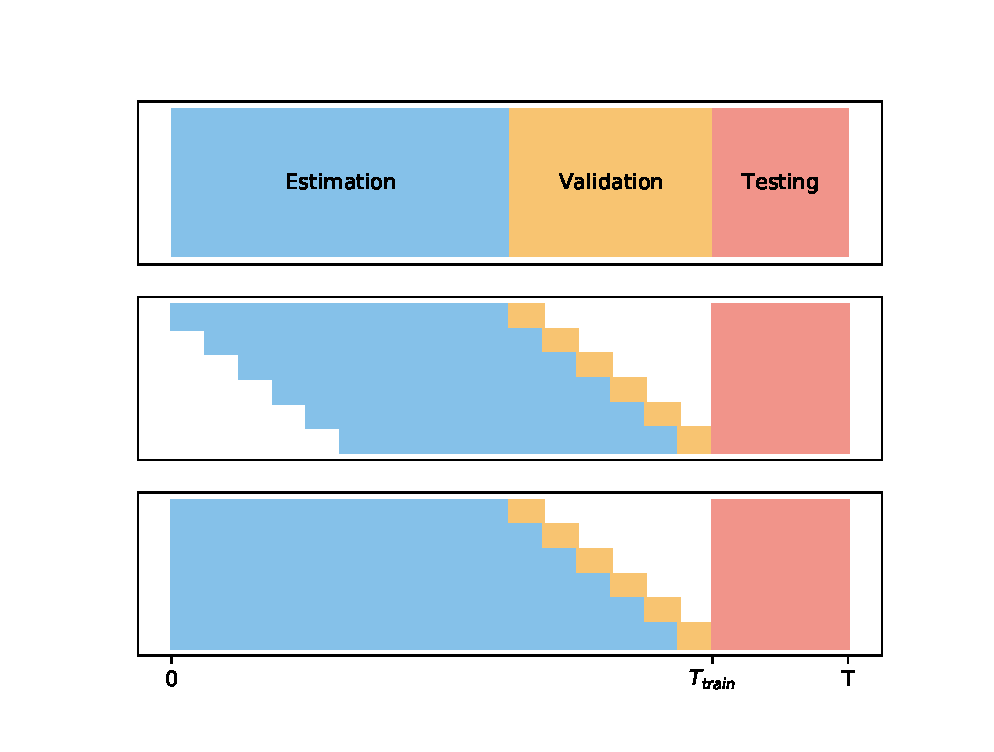
\includegraphics[width=\textwidth]{Plots/RollingExpandingWindow.eps}
    \end{center}
    \caption{The top panel describes the split of the avaliable data into an estimation and validation (which together is the training set) and a testing set, that is used to compare different models. The split was chosen $50\%$, $30\%$ and $20\%$, respectively. The center panel presents the rolling window approach and the expanding window approach is in the lower panel, both for a $6$-fold cross-validation technique that corresponds to a $5\%$ validation for each validation and a total of $30\%$ for the whole validation set. In the rolling window approach the size of the training set stays constant whereas in the expanding window approach, the effective training sample size increases.}
    \label{FIG:RollingExpanding}
\end{figure}

There are other approaches of cross-validation like random sampling or leave-$k$-out cross validation but those do not take into account the temporal nature of the data \citep{hastie01statisticallearning}. It would be unreasonable to estimate a temporal model on a given timeframe and validate its performance on data that preceeds the training set because there are dependencies over time and it would not be a realistic setting for making predictions into the future.
The rolling window and expanding window approach, however, take the time series setting into account and the training set temporally always preceeds the validation set. In the rolling window approach, the size of the estimation and validation set stays the same, because both are shifted over time. The expanding window on the other hand only has a constant validation set but the estimation set is increasing. This poses the challenge of inconsistent validation errors, because increasing the training has an impact on the quality of the estimation and therefore influence the validation error\footnote{This can come in both forms, better estimation which would decrease the validation error or overfitting which would increase the validation error.}. After cross validation has been performed and a set of hyperparameters has been fixed, the model can then be re-estimated on the whole training set to achieve the best estimation possible.

For the case of Echo State networks the hyperparameter optimization is performed in two steps because of the temporal and iterative nature of the network. When $\wout$ is estimated 'offline', the network activations $x_t$ have to be gathered in a matrix and this can only be done after the hyperparameters of the network, namely the spectral radius $\rho$ and the bias $\bb$, have been fixed. Based on the network activations, the regularization strength $\lambda$ of for example a ridge regression can be chosen accordingly.

The approach to the search for the best hyperparameters can be performed by simple grid search over a predefined set of hyperparameters. Alternatively, there are many computational packages that provide more sophisticated approaches like particle swarm optimization \citep{basterrech2015experimental} or gradient descent \citep{JAEGER2007335} as already mentioned in section \ref{CH:ESN:Hyperparameters}. For our empirical application we are going to use a \textit{gradient boosted regression tree} as part of a powerful Python packaged called \textit{scikit-optimize}\footnote{The package hasn't been maintained for quite some time, but has been taken over in January 2020. https://scikit-optimize.github.io/stable/}. The theory of regression trees and how to boost them are provided in \cite{hastie01statisticallearning}.


\subsection{Forecasting}

The models - both Echo State Networks and HAR - are trained to perform 1-step ahead predictions, this means $u_t = By_t$ for a times series $\left(y_t\right)_{t\in\Z}$. In order to come up with mutli-step ahead forecasts of horizon $h > 1$, we let the model produce a 1-step ahead forcast and feed the value back to the network as a new input. Assume, we have trained our model using data $\left(u_t\right)_{t\leq \ttrain}$ and we produce a 1-step ahead forecast $\hat y_{\ttrain+1}$. By concatenation and without retraining the model, we let it produce another 1-step ahead forecast based on $\left(..., u_{T-1}, u_T, \hat u_{\ttrain+1}\right)$. In an iterative way, this can produce an $h$-step ahead forecast $\hat u_{T+h}$.
One phenomenon that hasn't been researched extensively is the fact that injecting noise into the system while performing a multi-step prediction can improve performance. \cite{Jaeger2005} mentions that the injection of noise while updating the network can improve network stability. This can also be used in multi-step predictions. During the training of an Echo State Network, or more specifically in the training of $\wout$, you commit an error in the estimation. Using the residuals, which we will refer to as $e_t = y_t - \wout x_t$, $t = 1, ..., \ttrain$, of the estimation of what boils down to a linear regression, one can improve the performance by adding random draws of $\left\{e_1,...,e_{\ttrain}\right\}$. So instead of using the 1-step ahead prediction $\hat y_{\ttrain+1}$, you disturb the prediction and feed $\tilde u_{T+1} = \hat u_{T+1} + e_{j}$ to the network for a random draw $j \in \left\{1,...,\ttrain\right\}$. Finally, taking a monte carlo approach by producing multiple paths of $\left(\hat y_{\ttrain+1},..., \hat y_{\ttrain+h}\right)$ and averaging over those paths, the performance can be improved.% The number of prediction paths has to be chosen carefully, as too many simulations can negatively impact the predictive performance. In our empirical analysis the number of paths was chosen to be the same as $h$, the number of out-of-sample prediction steps.

\subsubsection{Fixed Training Set}
\label{CH:Application:Forecasting:Fixed}

We will not let the models predict the whole testing set in one go by the methods mentioned above, our testing set will be of size $1000$, but instead are going to take an iterative approach. As for the linear regression in the HAR model and the estimation of $\wout$ in the Echo State Networks, we will use fixed training set (consisting of estimation and validation) to estimate a cross-validated set of hyperparameters and regression parameters and those will not be changed over the course of the prediction. Given a forecasting horizon $h \in \left\{1,2,5,10\right\}$, we will start by letting the models predict $(\hat y_{\ttrain +1}, ..., \hat y_{\ttrain + h})$ as a set of iterated 1-step ahead forecasts if $h > 1$. We will then update the models by presenting them the true values $(y_{\ttrain +1}, ..., y_{\ttrain + h})$. Using the true data we will update the network state (for ESNs) and, in case of the experts, their weighting based on the associated loss over the period $[\ttrain +1, \ttrain + h]$. For the HAR model, we will update the regressors. For the plasticity, we are in fact able to update the weighting in a multistep prediction because the network state and its likelihood can be measured, independent of whether the true data or self-produced prediction has been fed or the network has been presented the true data. Once, the true data has been presented to the \textit{plasticity experts}, the network's reaction to its own predictions is rectified by the true data. Accordingly, the procedure then continues to produce forecasts $(\hat y_{\ttrain + h +1}, ..., \hat y_{\ttrain + 2h})$. This way, we can predict up to $\hmax = 1000$.
For both approaches we consider the mean error and the mean likelihood over the previous $h$ steps to update the weights in the multi-step prediction settings.

\subsubsection{Rolling Training Set}
\label{CH:Application:Forecasting:Rolling}

In contrast to the fixed training set approach, an alternative way of producing forecasts of the testing set is to re-estimate the models after every $h$-step ahead prediction. Since the optimization of hyperparameters weighs heavily on the training time, you usually stick to one set of hyperparameters that has been selected based on the training set. This makes a diligent selection of those parameters even more important. Keeping the hyperparameters, we will  however update the regression coefficients, namely $\wout$ for ESNs and $\bbeta$ for the HAR model. This way, we are able to account for regime changes in the time series, which are assumed to have no material effect on the set of hyperparameters.
For this approach, one can choose either the rolling window approach or the expanding window approach, now in relation to forecasting instead of hyperparameters optimization, as presented in figure \ref{FIG:RollingExpanding}.

\section{Empirical Results}
\label{CH:EmpiricalResults}


For the empirical application of the proposed model, we investigate the evolution of the IBM stock price. The data comes from the TAQ database of the New York Stock Exchange in the period from January 2nd, 2001 to December 30th, 2018. The price is sampled in intervals of $5$ minutes and contains $4444$ trading days, excluding holidays and weekends. The time series for our application will be the daily realized volatility introduced in section \ref{CH:Application:RV}. In order to compare the models that come from the Reservoir Computing field with the HAR model by \cite{Corsi2009}, we take the log transformation of the daily realized volatility. So our time series becomes
\begin{eqnarray}
    u_t = \log{\sqrt{RVD_t}} = \log{\sqrt{\sum_{j=1}^{78} r_{t_j}^2}}
\end{eqnarray}
where $r_{t_j}$ is referring to the $j$-th $5$-minute return on day $t$. The core trading hours on the New York Stock Exchange are from 9:30 am to 4:00 pm\footnote{https://www.nyse.com/markets/hours-calendars}, which amounts to $6.5$ hours or $87$ intervals of $5$ minutes.

Figure \ref{FIG:IBMRVAR:Series} presents the evolution of the realized volatility of IBM in the given timeframe. The left panel is referring to the original series of $\sigma_t$ and the right panel is its log transformation $\log{\sigma_t}$. 

Especially in the early years of the 21st century, the aftermath of the burtst of the 'dot com' bubble are still present in the timeseries which IBM as a technology company was probably more affected than other companies as well as the effect of the global financial crisis of 2007/2008 where this specific company was less affected by than in the early years of the century. Calmer periods of low volatility can be seen in the years between 2004 and 2006 and between late 2012 and late 2015 which underlines the presence of clustering.

Apart from the idiosyncratic risks associated to IBM, the evolution shows the typical patterns of volatility in financial time series, namely clustering and high persistence. Clustering is describing the pheonomenon of periods of high volatility being followed by periods of low volatility. High persistence is referring to a high level of autocorraltion which is presented in figure \ref{FIG:IBMRVAR:Autocorr}. The blue shaded area covers the range of significant autocorrelation and is touched for the first time at approximately the $140$-th lag. This corresponds to more than $6$ months. 


\begin{figure}
    \begin{center}
        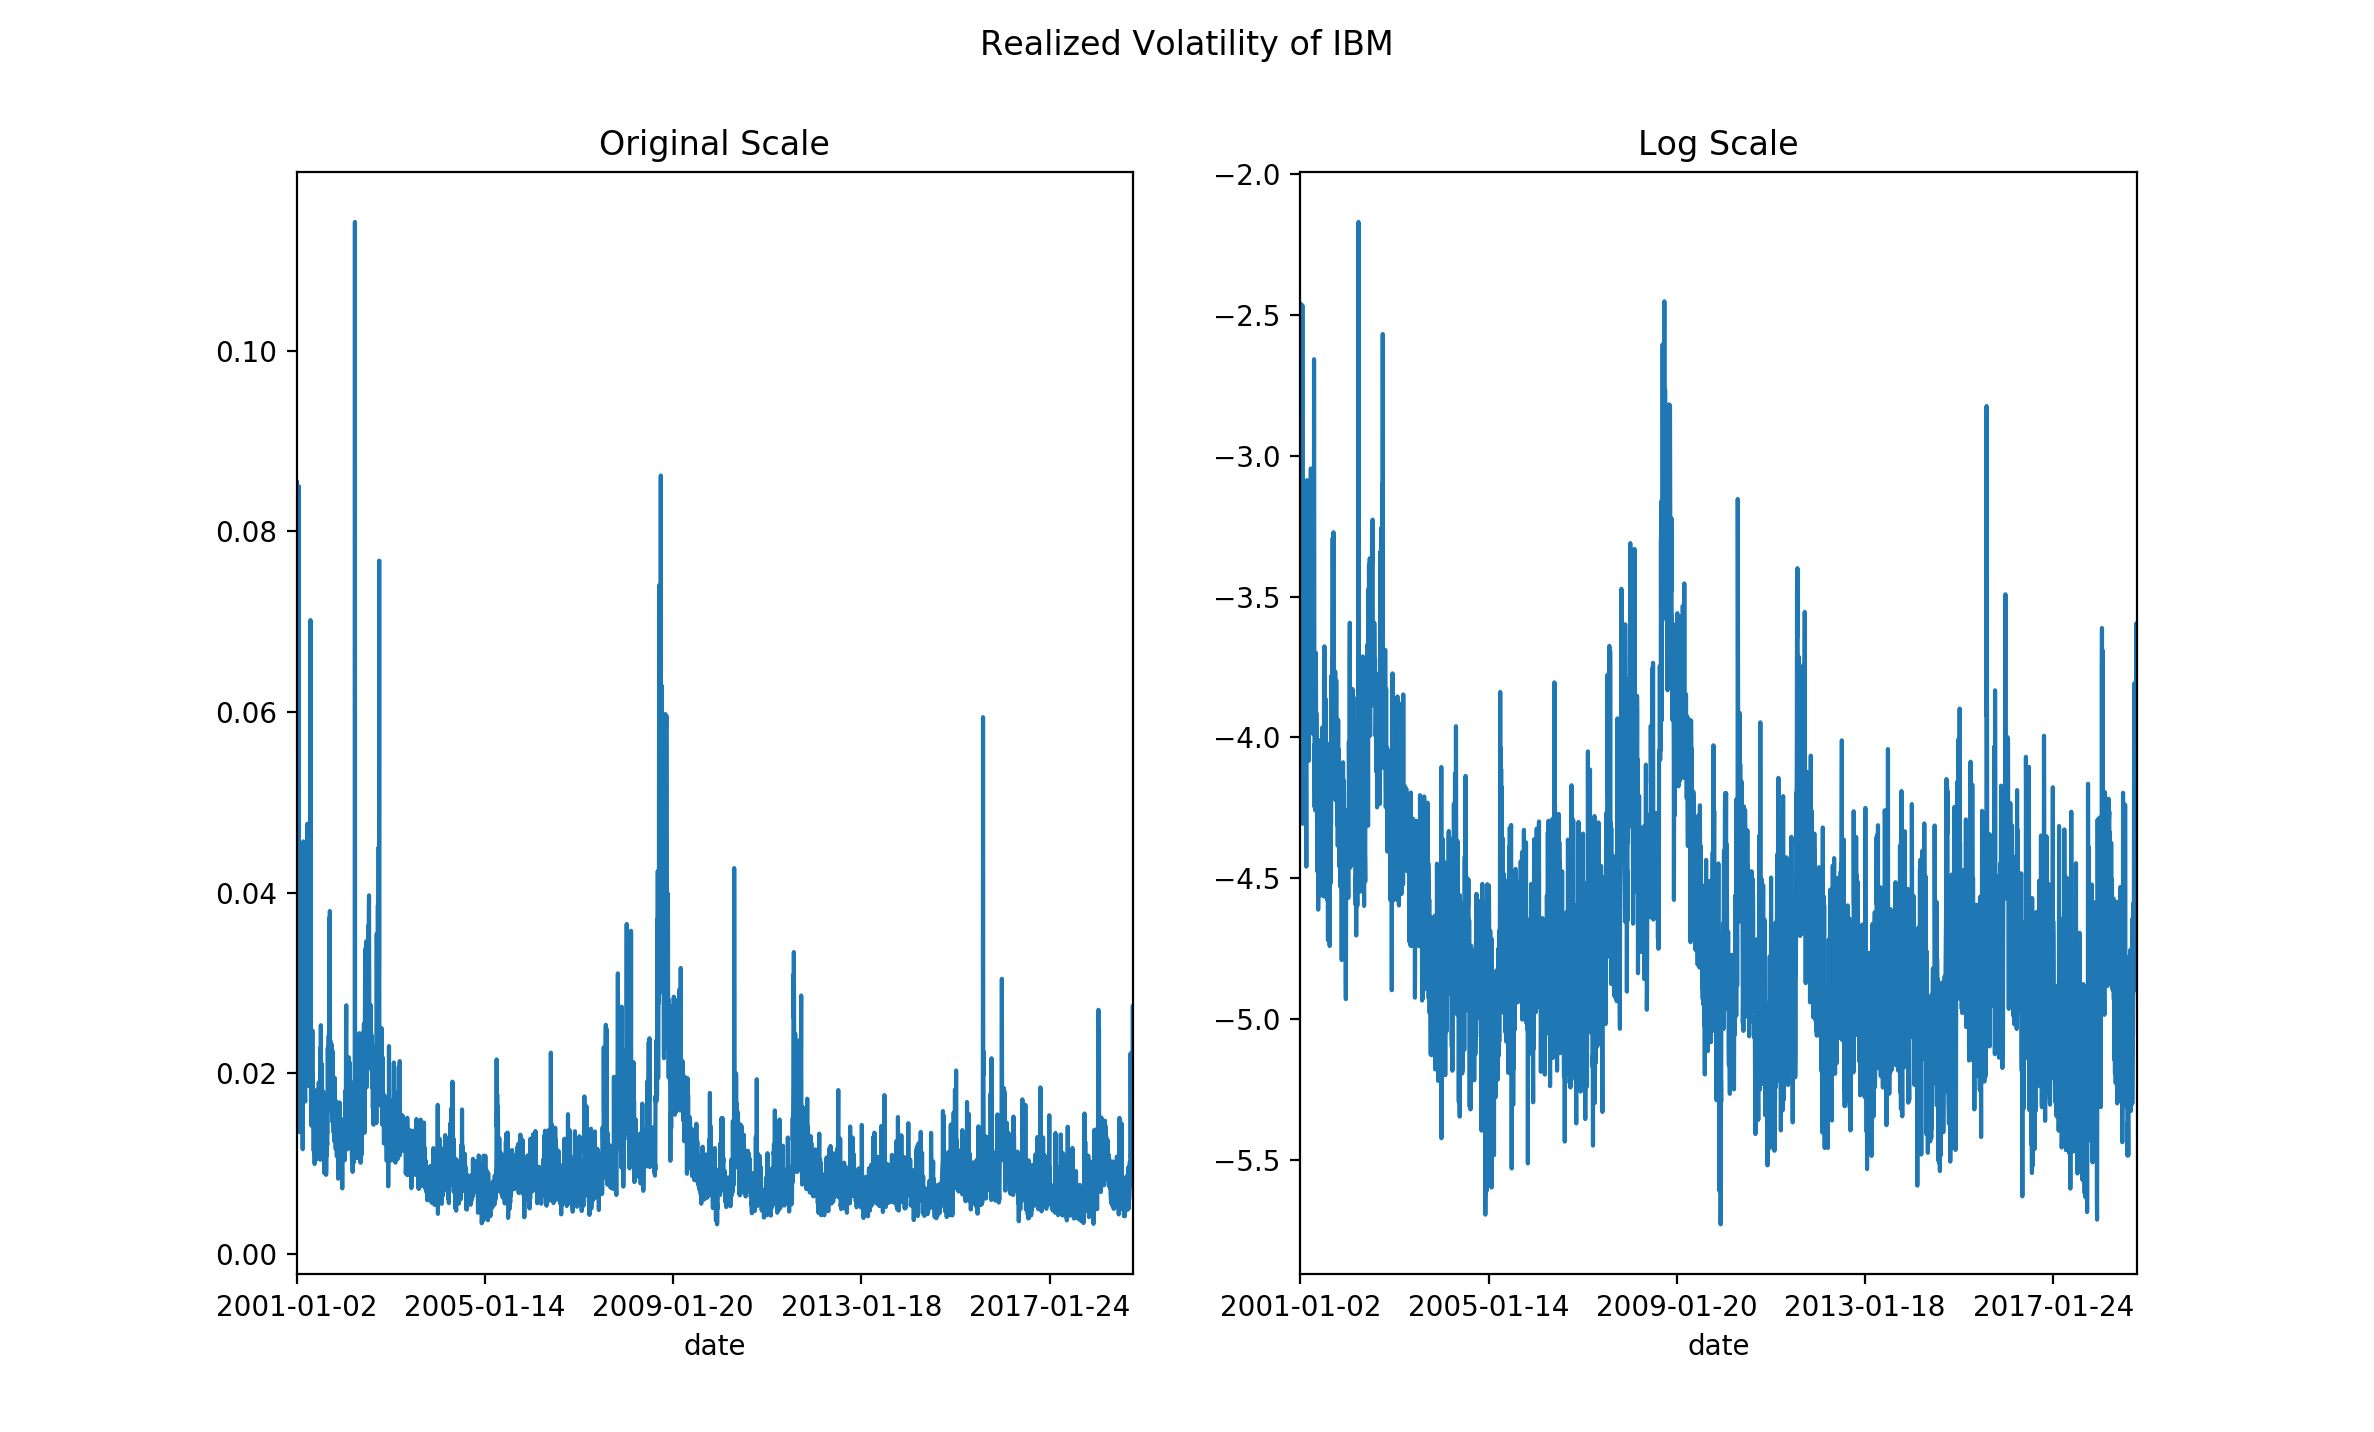
\includegraphics[width=\textwidth]{Plots/IBM_RVAR.png}
    \end{center}
    \caption{Realized volatility of IBM for the period from January 2nd, 2001 to December 30th, 2018. The left hand side presents the realized volatility in its original scale, the right hand side presents the log transformation of the time series.}
    \label{FIG:IBMRVAR:Series}
\end{figure}

\begin{figure}
    \begin{center}
        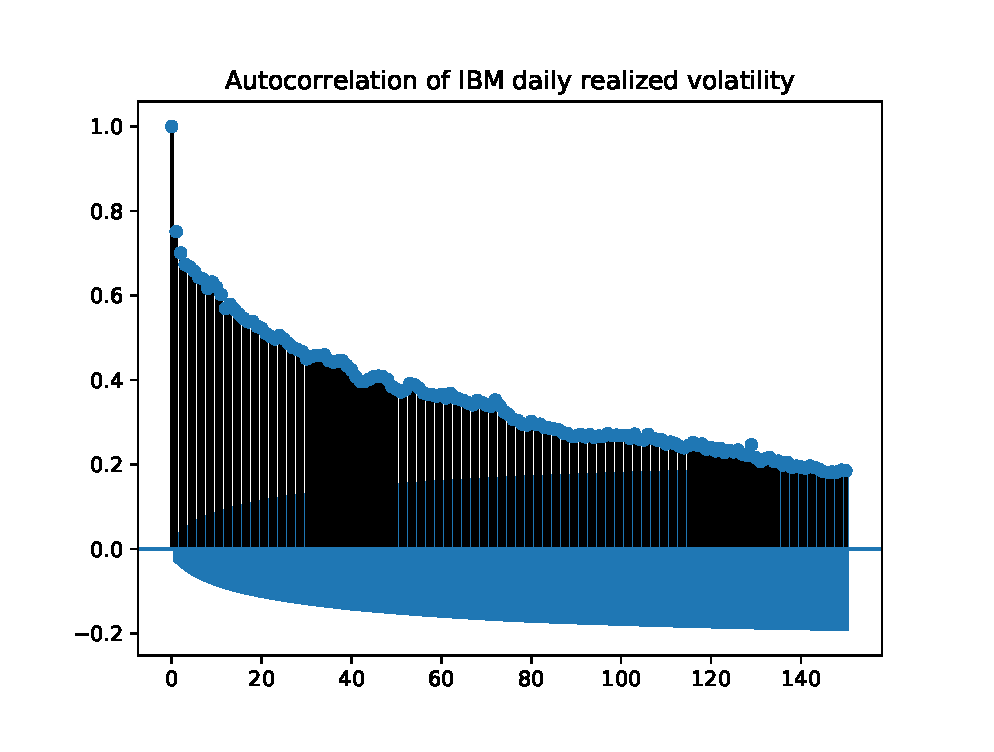
\includegraphics[width=\textwidth]{Plots/IBM_RVAR_autocorr.eps}
    \end{center}
    \caption{Autocorrelation of daily realized volatility of IBM for the period from January 2nd, 2010 to December 30th, 2018. The blue shaded area are the bounds for significance which is touched for the first time at approximately the $140$-th lag which shows the long persistence in the series.}
    \label{FIG:IBMRVAR:Autocorr}
\end{figure}

In what follows, we will refer to the loss induces experts as \textit{loss experts} and to the plasticity weighted experts as \textit{plasticity experts}.

\subsection{Analysis of Network Behaviour}

In this section we want to shed some more light of the network behaviour for reservoirs that have been pre-trained using the intrinsic plasticity approach from section \ref{CH:ESN:Tuning} using the IBM realized volatility as input $u_t$.
Figure \ref{FIG:NetworkActivations} presents the network activations for a givent time period and compares two networks that have been pre-trained towards different normal distributions. Networks of size $n=200$ were used and the network has been presented the whole time series of realized volatilities for $100$ epochs of adaptation. Given the $tanh$ activation function as well as the scaling of the input series to $[-0.8, 0.8]$ support the centering of network activations around $0$ which is in line with setting the mean $\mu = 0$ that has been argued about in section \ref{CH:ExpertModels}. The network behaviour for the left panel, which has been targeted towards $\mathcal{N}(0, 0.16)$, barely manages to put the neurons' output inside the $95\%$ confidence bounds of the respective normal distribution. In periods of relatively low volatility, e.g. between step $10$ and $20$ or around step $90$, the network is able to fit the normal distribution relatively well. This compares to the network in the right panel, where the network has been trained to match a normal distribution $\mathcal{N}(0,1)$. Here the adaptation barely manages to fit the neurons activations outside the confidence bounds\footnote{Given the size of the reservoir, approximately $0.05\cdot 200 = 10$ activations should lie outside the confidence bounds}.

% \begin{figure}
%     \begin{center}
%         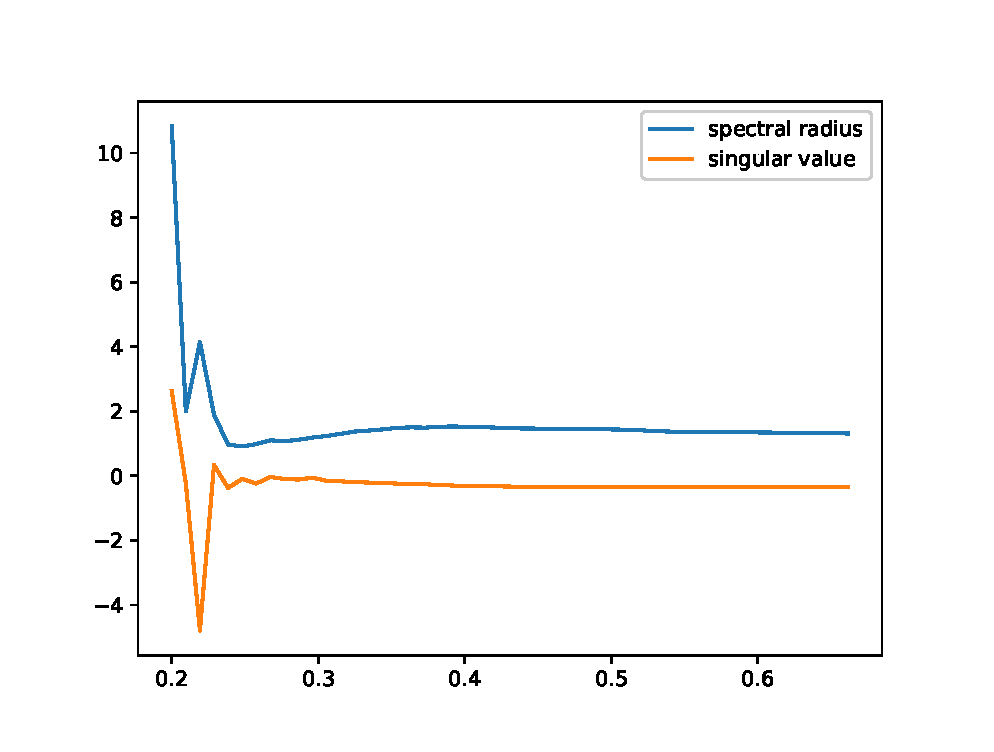
\includegraphics[width=\textwidth]{Plots/spectral_radius.eps}
%     \end{center}
%     \caption{foo}
%     \label{FIG:SpectralRadius}
% \end{figure}


\begin{figure}
    \begin{center}
        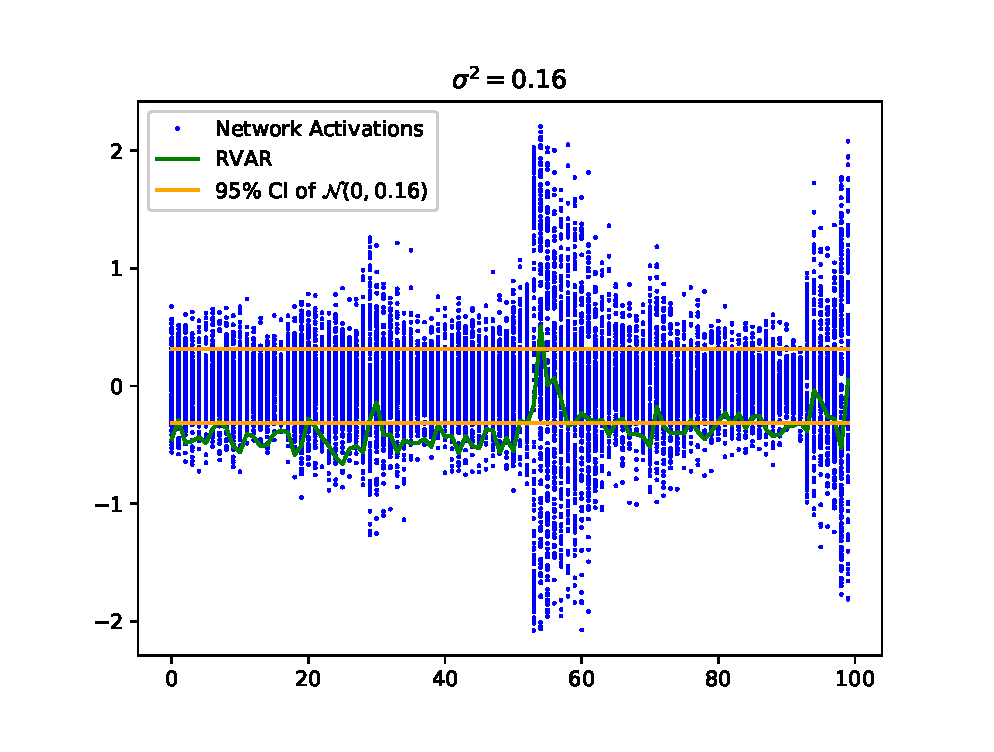
\includegraphics[width=0.49\textwidth]{Plots/network_activation_016.eps}
        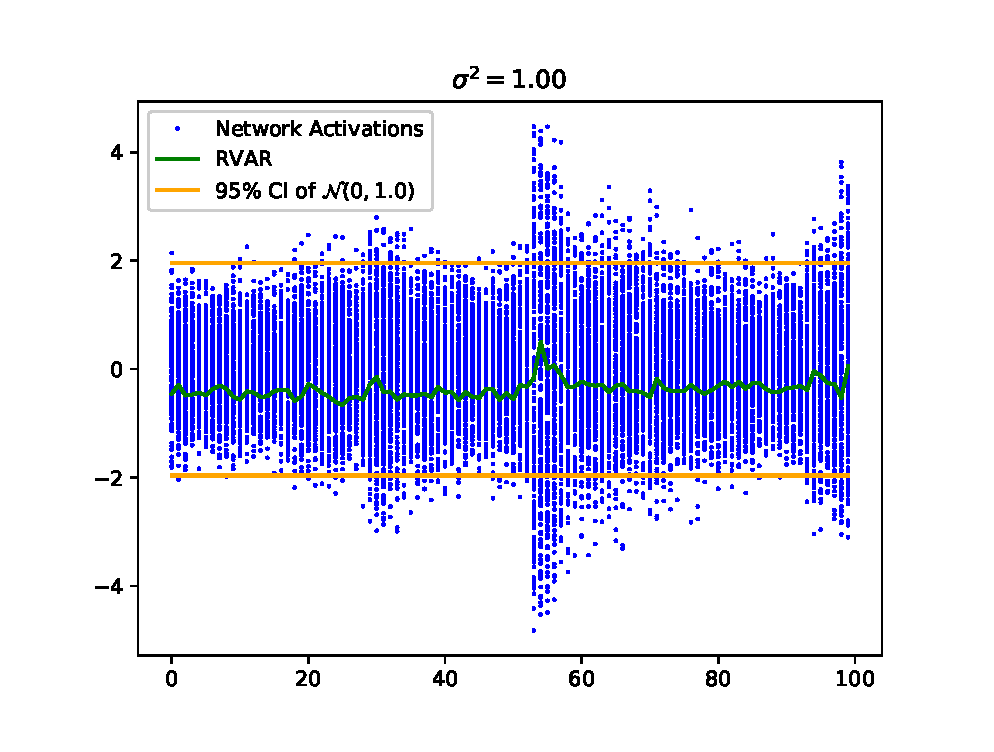
\includegraphics[width=0.49\textwidth]{Plots/network_activation_10.eps}
    \end{center}
    \caption{Comparison of the activations for two different plasticity tuned networks. One has been tuned for $\sigma = \frac{1}{\sqrt{2\pi}} = 0.16$ which we will use later in the empirical application. As a comparison, a network with $\sigma = 1.0$ is presented. The horizontal lines are the $95\%$ confidence bounds to give an idea of the range of a normal distribution $\mathcal{N}(0, \sigma^2)$ with the corresponding parameters. The time series presented is from 10th of July to 30th of October 2015. It has been rescaled to the interval $[-0.8, 0.8]$ and was chosen for representative purposes only. Comparing the two, one can see that the extreme values of the timeseries around step $55$ make the network with $\sigma = 0.16$ very unlikely given the amount of activations outside the confidence bounds. The effect of this move on the network with $\sigma = 1.0$ is much less significant when considering the comparably fewer activations outside the bounds. Intuitively, this makes sense because the higher volatility move in the time series would favor the network which allows for and targets a wider range of activations.}
    \label{FIG:NetworkActivations}
\end{figure}

Additionally, figure \ref{FIG:IBMRVAR} presents the evolution of the networks likelihood in relationship to the timeseries of a tuned network, in this case targeted to $\mathcal{N}(0,1)$. The likelihood, as the series before presenting it to the network, has been rescaled to the interval $[-0.8,0.8]$. The relationship between the series and the likelihood is clearly negative, the correlation coefficient is $-0.59$. Whenever the series is spiking, the likelihood is negatively impacted. This is in line with the analysis of figure \ref{FIG:NetworkActivations} which shows the same relationship of spikes and their impact on the likelihood. Given that the networks have been adapted to a series that rarely exhibits spikes, it is to be expected that all networks, independent of the targeted output distribution, show a negative correlation between the likelihood and the series itself. 
This, however, compares directly to the \textit{loss experts} approach where each expert is suffering an individual loss and their weighting is based on the relative loss and not the absolute loss. Therefore, the \textit{plasticity experts} are based on their relative likelihood and some network may have a stronger (negative) impact on the likelihood compared to another networks.
We expect the networks with an output distribution of higher volatility to favor instances where the time series experiences spikes and output distributions with comparatively lower volatility to favor more supressed regimes of daily realized volatility.


\begin{figure} 
    \begin{center}
        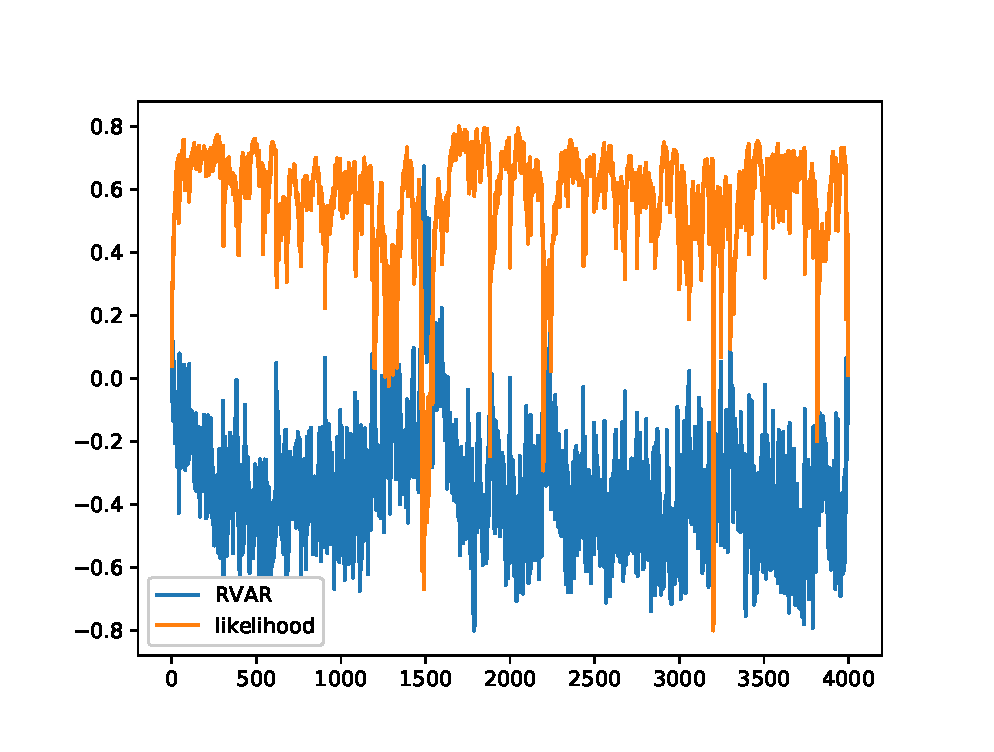
\includegraphics[width=\textwidth]{Plots/likelihood_evolution_1.eps}
    \end{center}
    \caption{The network activation and the corresponding likelihood of the activation for the pre-trained network with a target $\sigma = 1.0$. The correlation of the two series is $-0.59$. The likelihood has been rescaled to the same interval of $[-0.8, 0.8]$ as the series itself. One can clearly see the negative relationship of likelihood and the spikes in the series. Under \textit{normal} conditions, this means in times of low volatility, the likelihood is larger than at times where there is a spike in the series. This is to be expected because spikes are comparably rare and the network has mostly adapted to these low volatility regimes. The edge of the \textit{plasticity experts}, as with the \textit{loss experts}, is expected to be found in the relative likelihood and the networks' reaction to the spikes in the series and their resulting likelihoods.}
    \label{FIG:IBMRVAR}
\end{figure}


\subsection{Predictive Performance}

This section presents the empirical forecasting performance of the plasiticity approach in comparison to benchmark tasks including the HAR model by \cite{Corsi2009}, the exponential weighted experts of Echo State Network and a single Echo State Network with equivalent size and hyperparameter optimization that has been performed for the spectral radius $\rho$ and bias $\bb$.

\begin{table}
\begin{center}
    \begin{tabular}{l|c|c|c|c}
        & initial transient & training & validation & testing \\ \hline
        ESN & $444$ & $2700$ & \multirow{2}{*}{$300$} & \multirow{2}{*}{$1000$} \\
        \cline{1-3}
        HAR & \multicolumn{2}{|c|}{$3144$} & & 
    \end{tabular}
    \label{TABLE:TimeSeriesSplit}
\end{center}
\caption{Split of the timeseries into different parts during the empirical application. The echo state network approaches have an initial transient to wash out the initialization of the network state which - for the convenience of the other sets - was chosen as $444$. As the HAR model doesn't need this transient, those additional days are attributed to the training set which results in a larger training set of $3144$ days.}
\end{table}

The timeseries has been divided according to table \ref{TABLE:TimeSeriesSplit}. The initial transient is referring to the wash-out period of the Echo State Networks to reduce the effect of the 0-initialization of the network state which effectively decreases the training size. This, coming as a tradeoff compared to the HAR model, decreased the amount of data for the estimation because the the validation set was kept the same for the models. The size of the test set, $\hmax$, was set to $1000$ which corresponds to roughly $4$ years of daily data.



\subsubsection{Model Specifications}

Applying the new model, we will compare the following specifications and comparators:
\begin{itemize}
    \item HAR model by \cite{Corsi2009}
    \item ESN experts with loss functions:
    \begin{itemize}
        \item $L(\hat u_t, u_t) = (\hat u_t-u_t)^2$
        \item $L(\hat u_t, u_t) = (\exp{\hat u_t} - \exp{u_t})^2$
        \item $L(\hat u_t, u_t) = \frac{\exp{u_t}^2}{\exp{\hat u_t}^2} - \frac{u_t^2}{\hat u_t^2} - 1$
    \end{itemize} 
    in the exponential update of weights \ref{EQ:LossUpdate}
    \item Plasticity weighted experts with
    \begin{itemize}
        \item $\sigma_k = \frac{1}{\sqrt{2\pi}}$ for all $k = 1, ..., K$
        \item An equally spaced grid of $\sigma_k \in \left[0.8\left(2\pi\right)^{-\frac{1}{2}}, 1.2\left(2\pi\right)^{-\frac{1}{2}}\right]$ around the constant value $\frac{1}{\sqrt{2\pi}}$
    \end{itemize}
    \item Single ESN of comparable size where the hyperparemeter optimzation of the spectral radius $\rho$ and bias $b$ and their validation has been performed using tge same error functions as the experts approach
\end{itemize}
For the loss functions of the loss experts, one has to keep in mind the transformation $u_t = \log{\sqrt{\sigma_t^2}}$ of the timeseries by the square root and the natural logarithm. Hence, the three loss functions correspond to the differnt scales of the series, (i) the logarithm of the volatility $\log{\sigma}$, (ii) the volatility $\sigma$ and (iii) the variance $\sigma^2$.
The choice of $\sigma_k \equiv \frac{1}{\sqrt{2\pi}}$ is motivated by the plasticity update \refp{EQ:Likelihood}, so that the additional factor of $\frac{1}{\sqrt{2\pi\sigma_k^2}} = 1$. All the specifications are trained using the online learning of equations \refp{EQ:RLS1} - \refp{EQ:RLS2}. The choice of the range of spectral radii for the loss experts was motivated by the correspondence to the effective spectral radius of the plasticity experts which are in the range of $[0.8, 1.2]$. This is also supported by the fact that the single ESN with optimized hyperparameters was using a spectral radius of approximately $\rho \in [1.20, 1.25]$, depending on the loss function. Even though, we showed some relationship between the two approaches in section \ref{CH:ExpertModels:Equivalence}, a fair way of comparison still has to be found.


The following results are based on $K=10$ experts, total number of neurons $N=1000$, bias equal to $0.2$. In order to compare the models it is crucial, that the random number generator is fixed for all the applications. When this is neglected, by the nature of the reservoir computing models and their random initalization, the comparison of predictive performance may be due to the state of the random number generator when initializing the random connections and can actually not be attributed to the model design. This way, it can be guaranteed that the differences in performance can be attributed to the different weighting approaches and model specifications.
Beyond the random initialization, the networks of the \textit{plasticity experts} have been adapted to their targeted output distributions using $50$ epochs of presenting them the whole training data set.

The original scale of daily realized volatility was $[0.0032, 0.1142]$ which was log transformed to $[-5.7300, -2.1691]$. For the reservoir computing models, it was finally rescaled to $[-0.8, 0.8]$.


\begin{table}
    \begin{center}
        \begin{tabular}{|c|c|c|c|c|}
            \hline
            \multicolumn{2}{|c|}{}    & spectral radius & bias & regularization \\\hline
            \parbox[t]{2mm}{\multirow{3}{*}{\rotatebox[origin=c]{90}{Single}}} & logMSE & $1.0107$ & $0.4507$ & $20.7$ \\
            \cline{2-5}
            & MSE & $0.8142$ & $0.3711$ & $20.7$ \\
            \cline{2-5}
            & QLIKE & $0.8263$ & $0.8414$ & $6.2$ \\\hline
            \parbox[t]{2mm}{\multirow{3}{*}{\rotatebox[origin=c]{90}{Loss}}} & logMSE  & \multirow{3}{*}{$[0.2, 2.0]$} & \multirow{3}{*}{$0.2$} & $[0.5, 1.8]$  \\
            \cline{2-2}\cline{5-5}
            & MSE & & & $[0.0003, 1.8]$ \\
            \cline{2-2}\cline{5-5}
            & QLIKE & & & $[0.0003, 0.5]$ \\\hline
            \parbox[t]{2mm}{\multirow{2}{*}{\rotatebox[origin=c]{90}{Plast}}} & Constant & $[0.32, 1.51]$ & $[-31.2, 73.4]$ & $[0.5, 1.8]$ \\
            \cline{2-5}
            & Grid & $[0.31, 1.36]$ & $[-33.8, 67.0]$ & $[0.5, 1.8]$ \\
            \hline
        \end{tabular}
        \label{TABLE:SelectedHyperparameters}
    \end{center}
    \caption{Selected hyperparameters of the models based on the training dataset. For the plasticity experts, the spectral radius and the bias are referring to the effective quantities of the network dynamics after tuning them by the plasticity approach.}
\end{table}

The selected hyperparameters are presented in table \ref{TABLE:SelectedHyperparameters}. The highest and lowest values of the spectral radius and bias have been realized for the same networks, which means that there are some extreme networks and some less extremely modified network dynamics. The strong regularization in the Single ESN is to be expected given the larger size of $N = 1000$ neurons, compared to the experts that are only of size $N=100$, but the regularization of the QLIKE is comparably low at $6.2$ but may be attributed to the different combination of a lower spectral radius and a higher bias.




\subsubsection{Fixed Training Performance}
\label{CH:EmpiricalResults:Fixed}

This section presents the out-of-sample predictive performance of the models referring to section \ref{CH:Application:Forecasting:Fixed} where the models have only been trained on the training set, which is up to $\ttrain = 3444$, and have not been re-estimated for the predictions.

\begin{figure}
    \begin{center}
        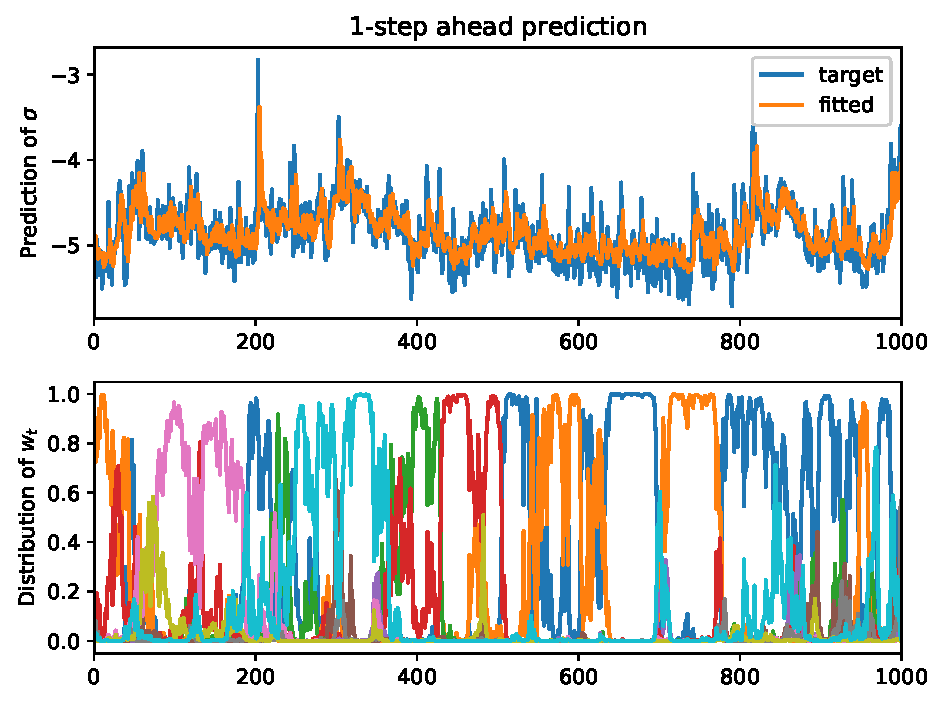
\includegraphics[width=0.45\textwidth]{Plots/Prediction/Experts_logMSE_1step.eps}
        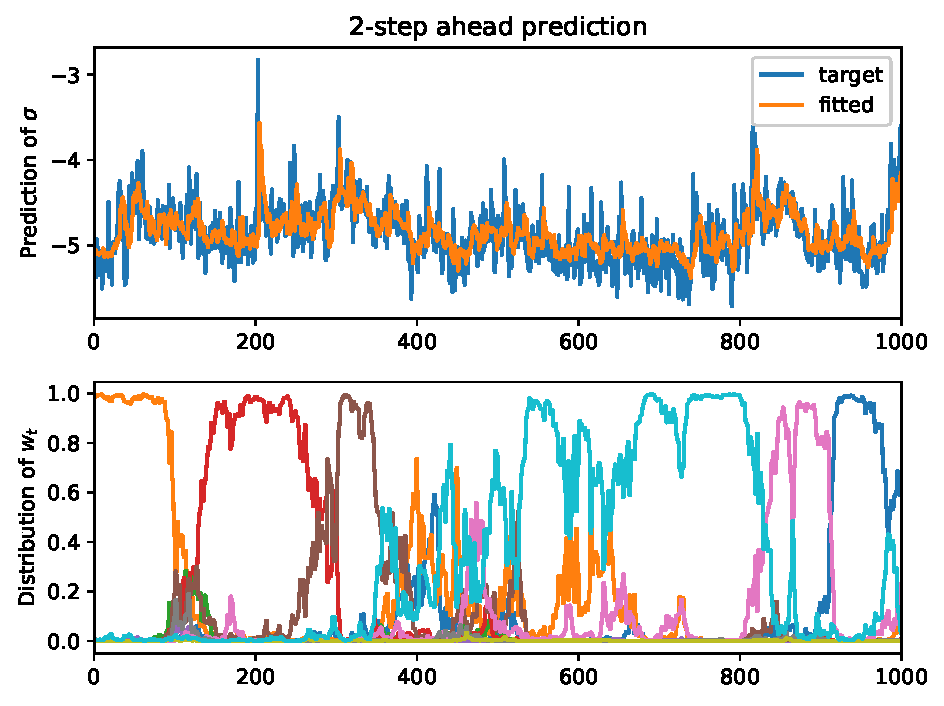
\includegraphics[width=0.45\textwidth]{Plots/Prediction/Experts_logMSE_2step.eps} \\
        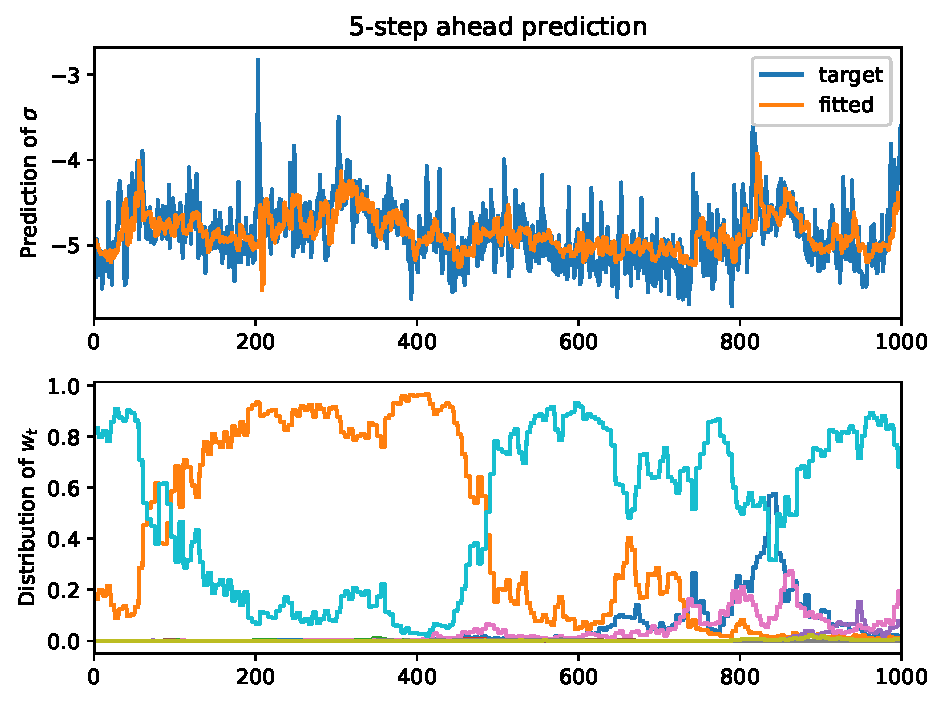
\includegraphics[width=0.45\textwidth]{Plots/Prediction/Experts_logMSE_5step.eps}
        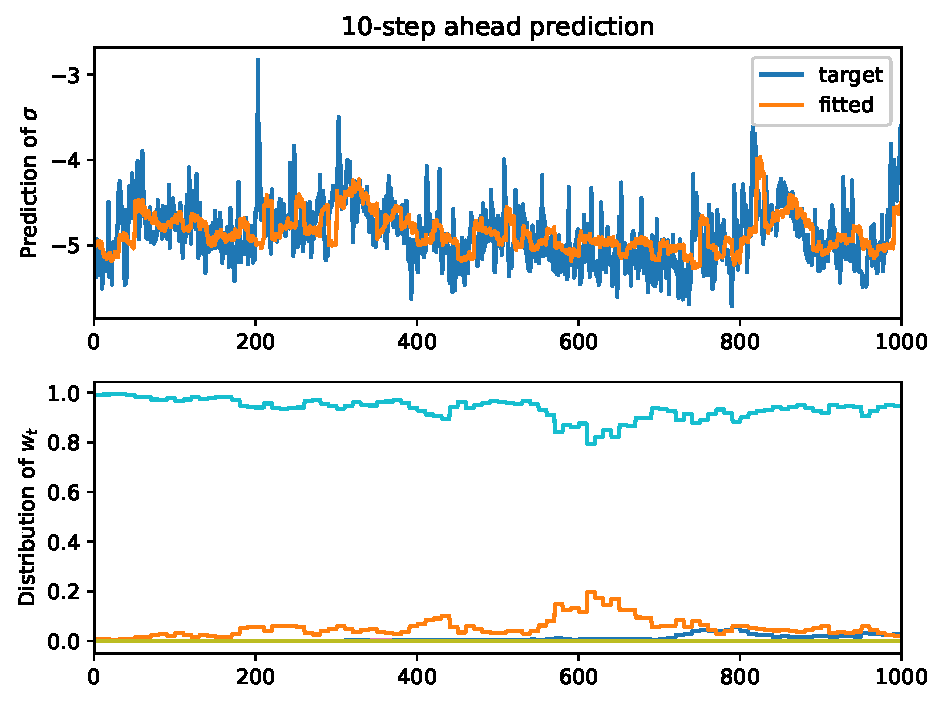
\includegraphics[width=0.45\textwidth]{Plots/Prediction/Experts_logMSE_10step.eps} \\
        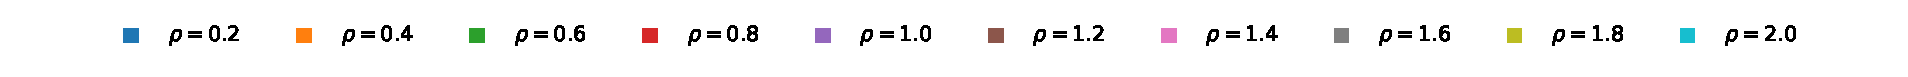
\includegraphics[width=1.0\textwidth]{Plots/Prediction/legend_experts.eps}
        \label{FIG:ExpertsLogMSE}
    \end{center}
    \caption{This is the \textit{loss experts} approach with exponential weighting of the experts based on the mean squared error of the log transformation $\log{\sigma}$. The values of spectral radii are equally space in the interval $\rho \in [0.2, 2.0]$. The networks have only been trained once on the training set as outlined in section \ref{CH:Application:Forecasting:Fixed}.}
\end{figure}

\begin{figure}
    \begin{center}
        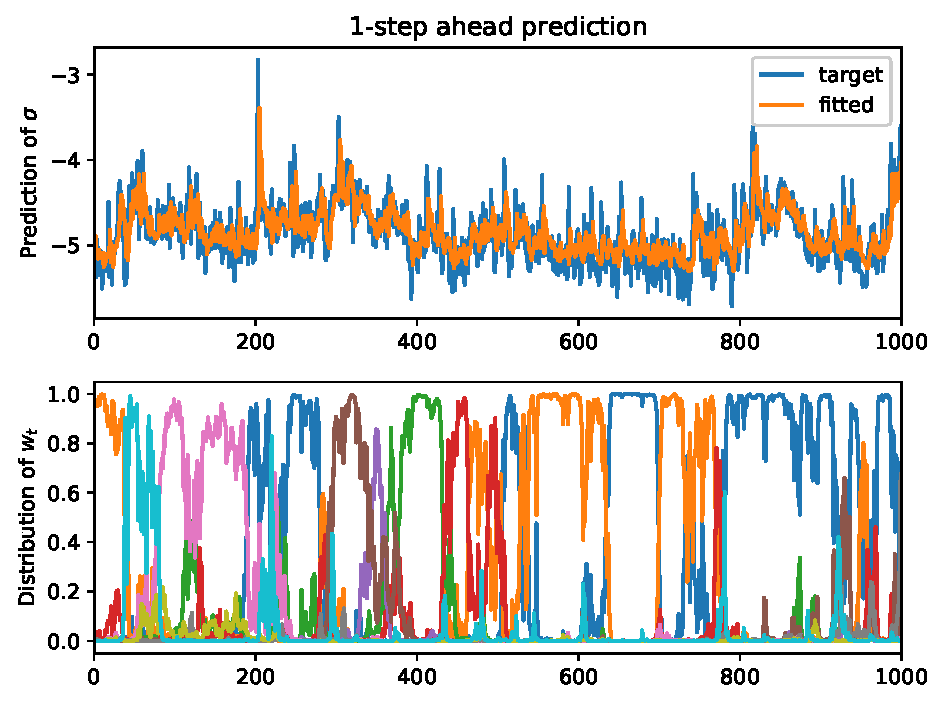
\includegraphics[width=0.45\textwidth]{Plots/Prediction/Experts_MSE_1step.eps}
        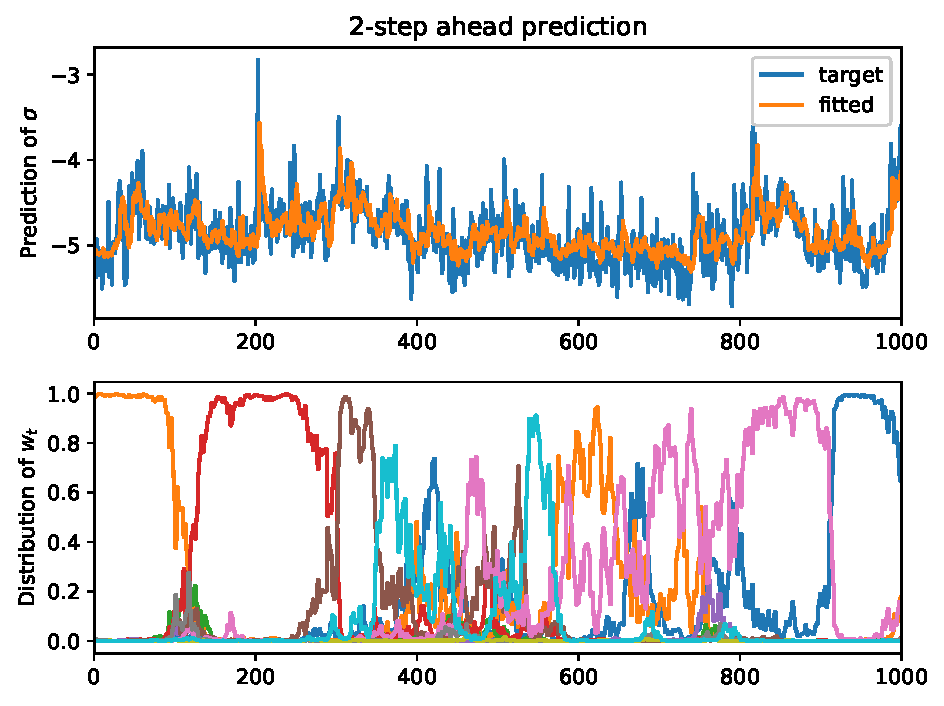
\includegraphics[width=0.45\textwidth]{Plots/Prediction/Experts_MSE_2step.eps} \\
        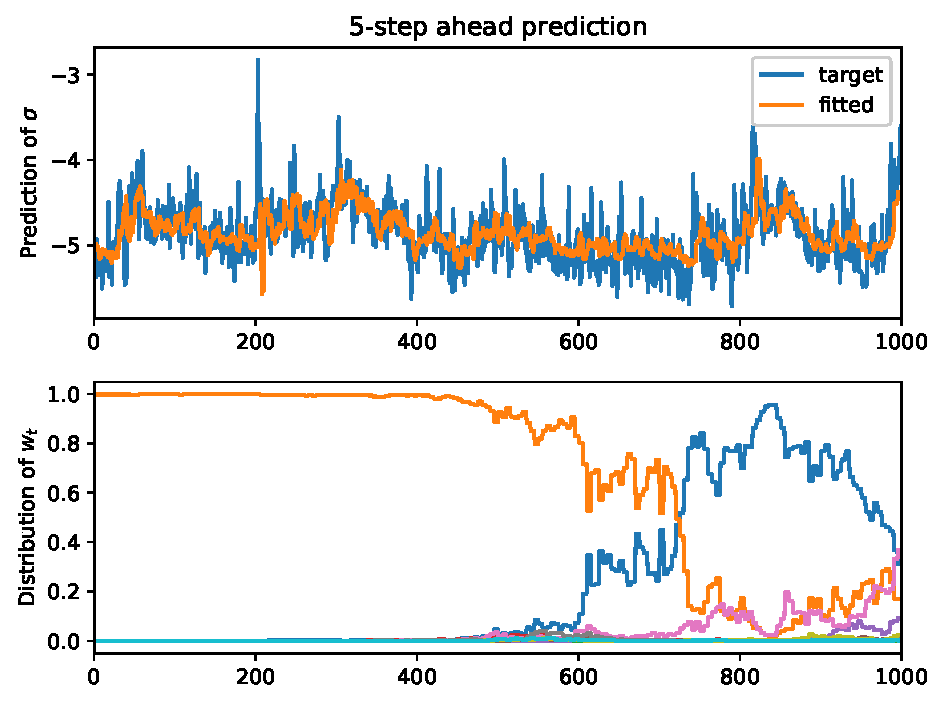
\includegraphics[width=0.45\textwidth]{Plots/Prediction/Experts_MSE_5step.eps}
        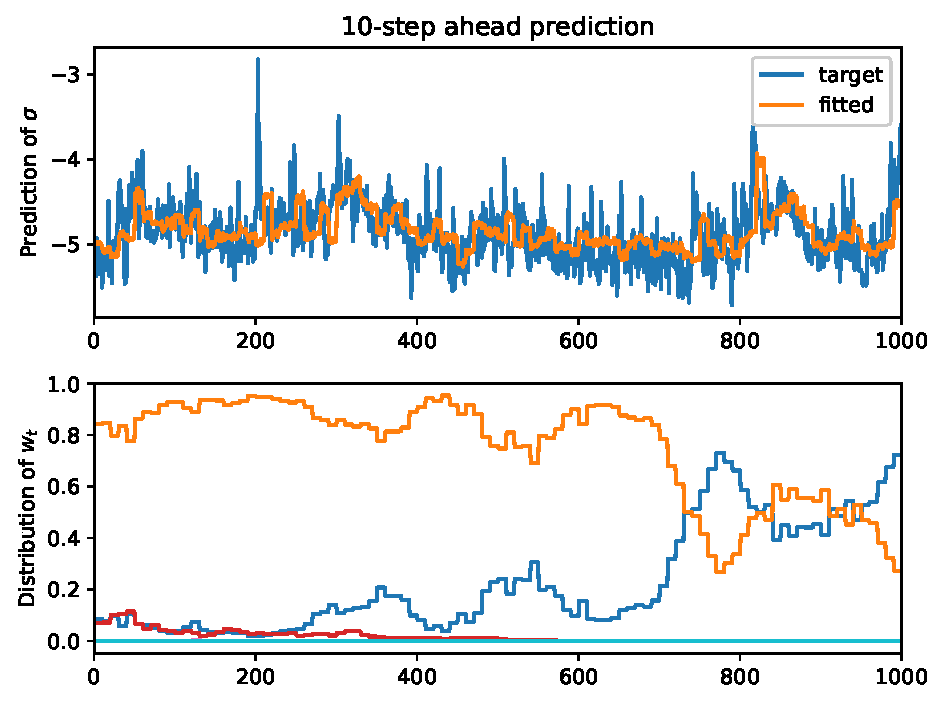
\includegraphics[width=0.45\textwidth]{Plots/Prediction/Experts_MSE_10step.eps} \\
        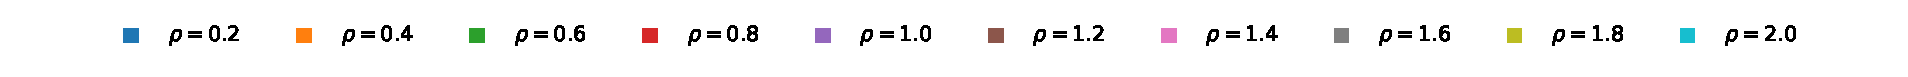
\includegraphics[width=1.0\textwidth]{Plots/Prediction/legend_experts.eps}
        \label{FIG:ExpertsMSE}
    \end{center}
    \caption{This is the \textit{loss experts} approach with exponential weighting of the experts based on the mean squared error of the original time series, so $\sigma$. The values of spectral radii are equally space in the interval $\rho \in [0.2, 2.0]$. The networks have only been trained once on the training set as outlined in section \ref{CH:Application:Forecasting:Fixed}.}
\end{figure}

\begin{figure}
    \begin{center}
        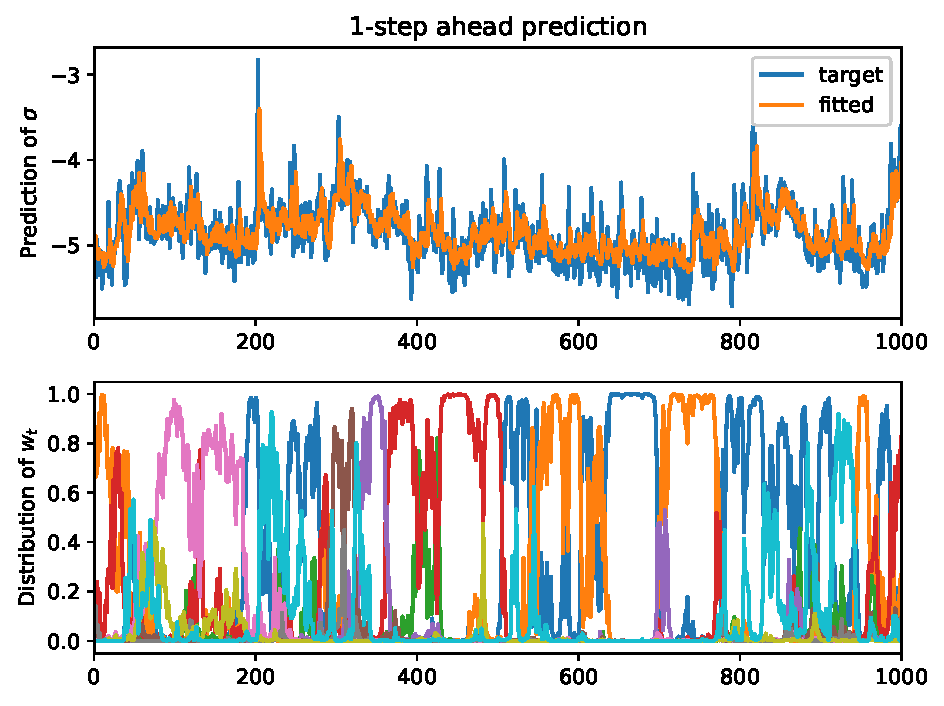
\includegraphics[width=0.45\textwidth]{Plots/Prediction/Experts_QLIKE_1step.eps}
        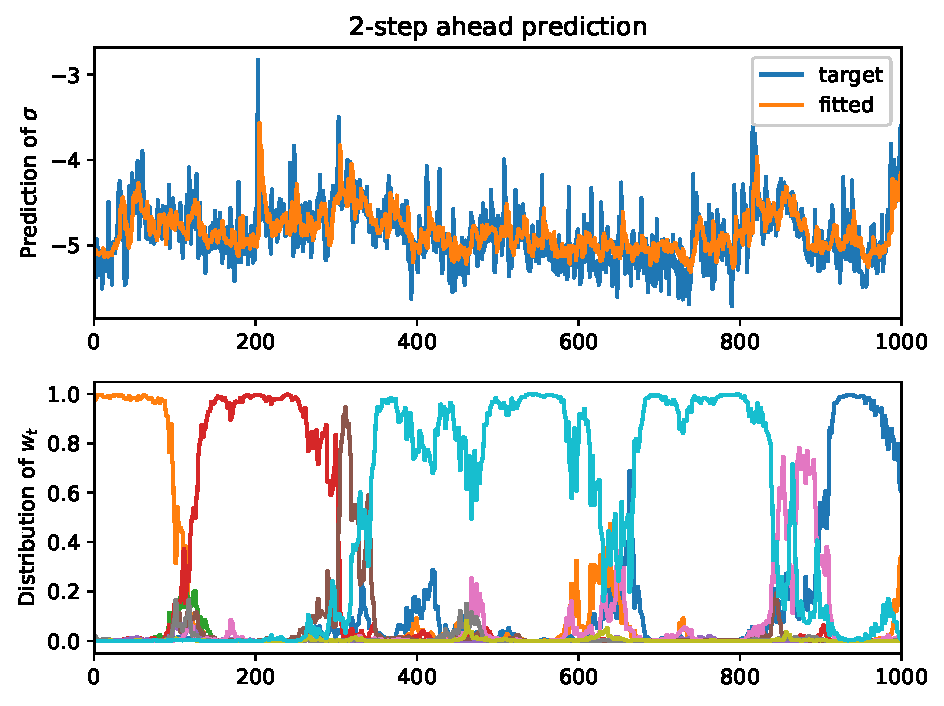
\includegraphics[width=0.45\textwidth]{Plots/Prediction/Experts_QLIKE_2step.eps} \\
        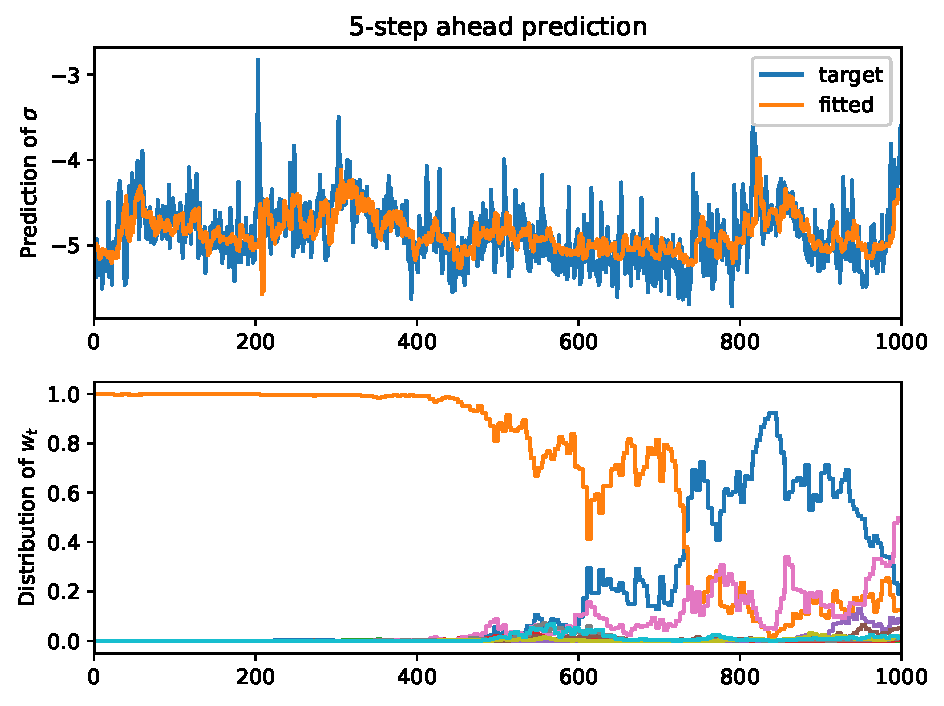
\includegraphics[width=0.45\textwidth]{Plots/Prediction/Experts_QLIKE_5step.eps}
        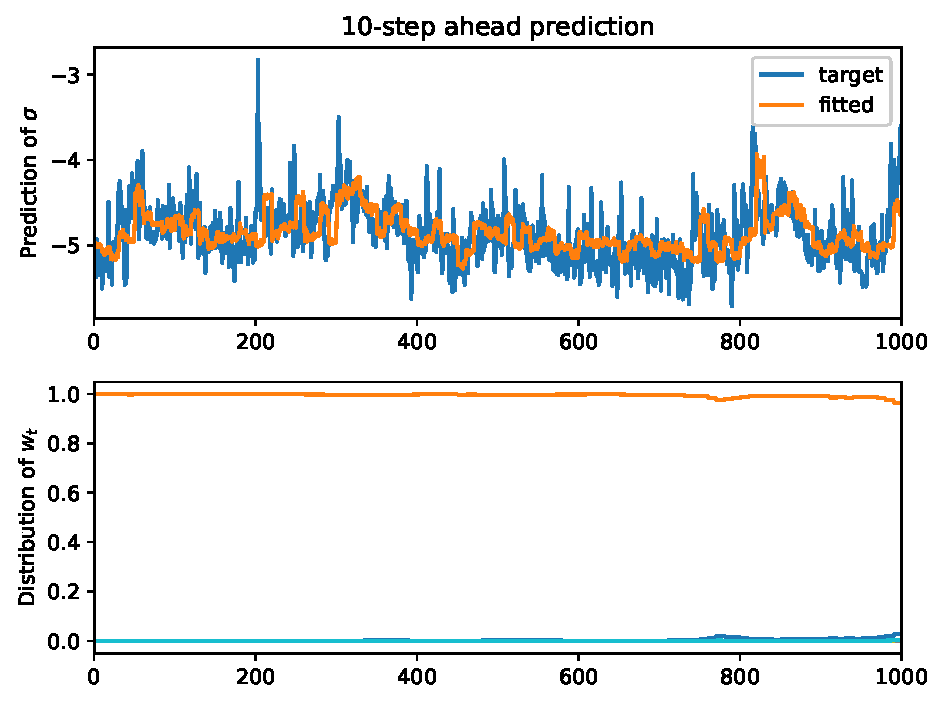
\includegraphics[width=0.45\textwidth]{Plots/Prediction/Experts_QLIKE_10step.eps} \\
        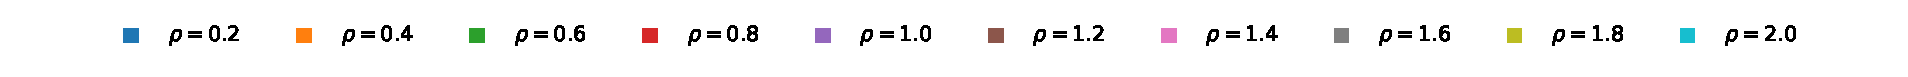
\includegraphics[width=1.0\textwidth]{Plots/Prediction/legend_experts.eps}
        \label{FIG:ExpertsQLIKE}
    \end{center}
    \caption{This is the \textit{loss experts} approach with exponential weighting of the experts based on the QLIKE loss function, so in the scale of $\sigma^2$. The values of spectral radii are equally space in the interval $\rho \in [0.2, 2.0]$. The networks have only been trained once on the training set as outlined in section \ref{CH:Application:Forecasting:Fixed}.}
\end{figure}


\begin{figure}
    \begin{center}
        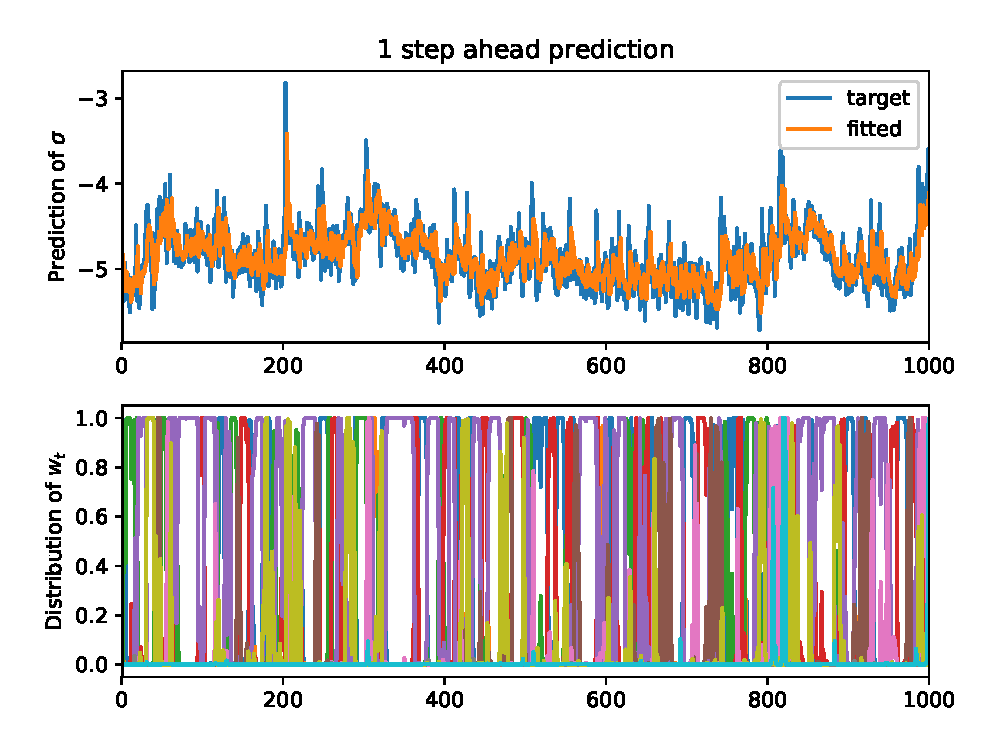
\includegraphics[width=0.45\textwidth]{Plots/Prediction/Plasticity_Constant_1step.eps}
        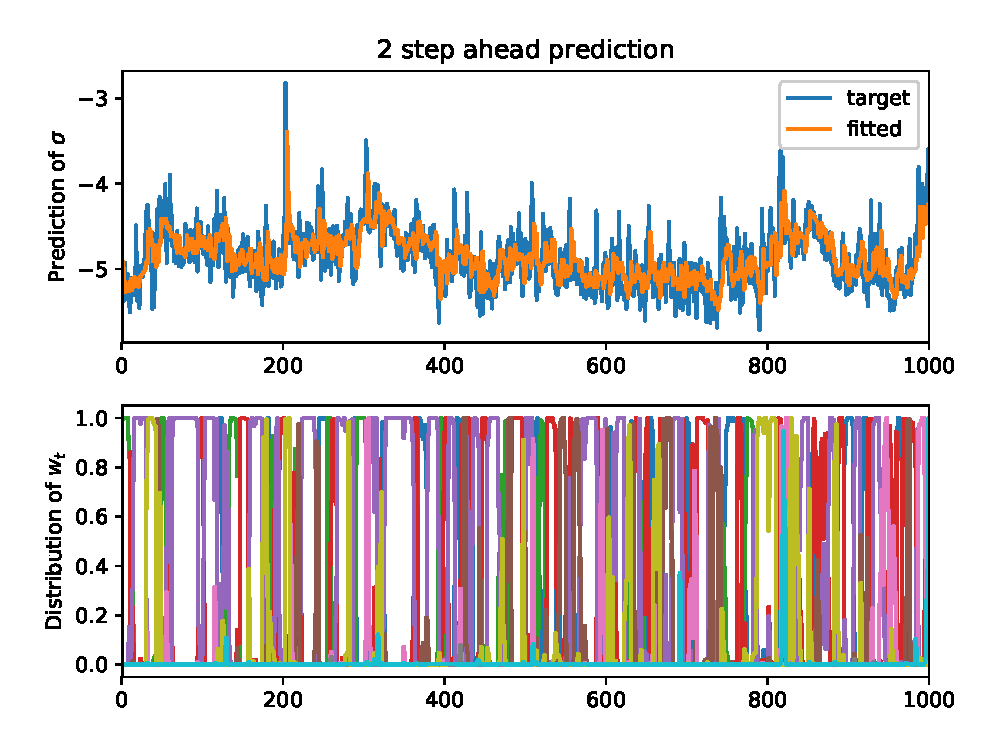
\includegraphics[width=0.45\textwidth]{Plots/Prediction/Plasticity_Constant_2step.eps} \\
        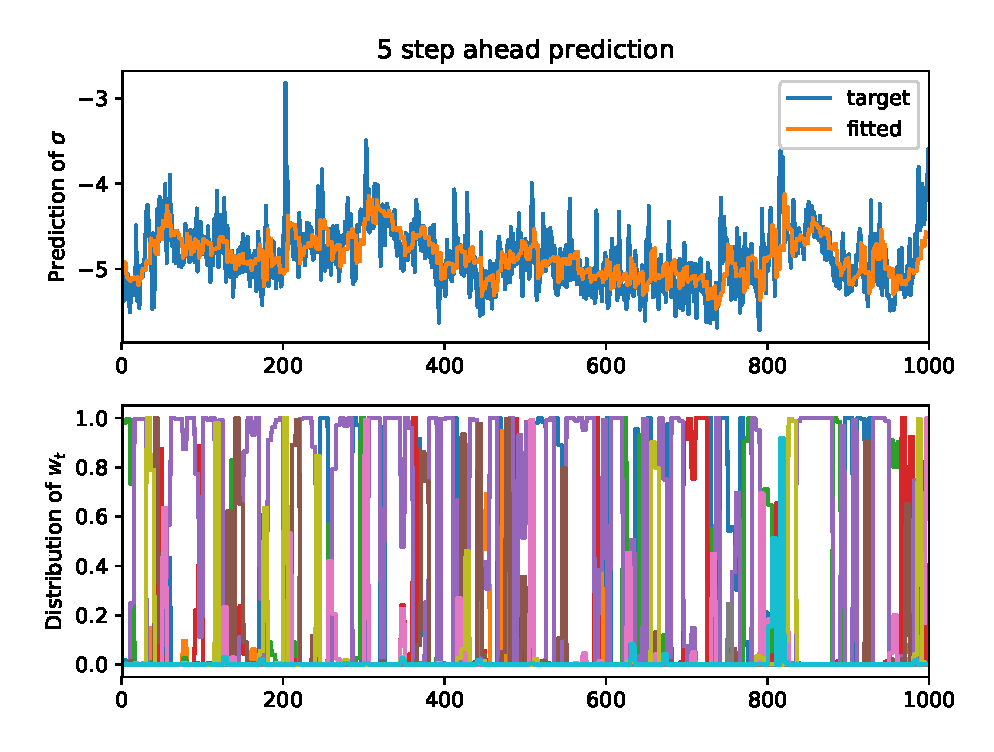
\includegraphics[width=0.45\textwidth]{Plots/Prediction/Plasticity_Constant_5step.eps}
        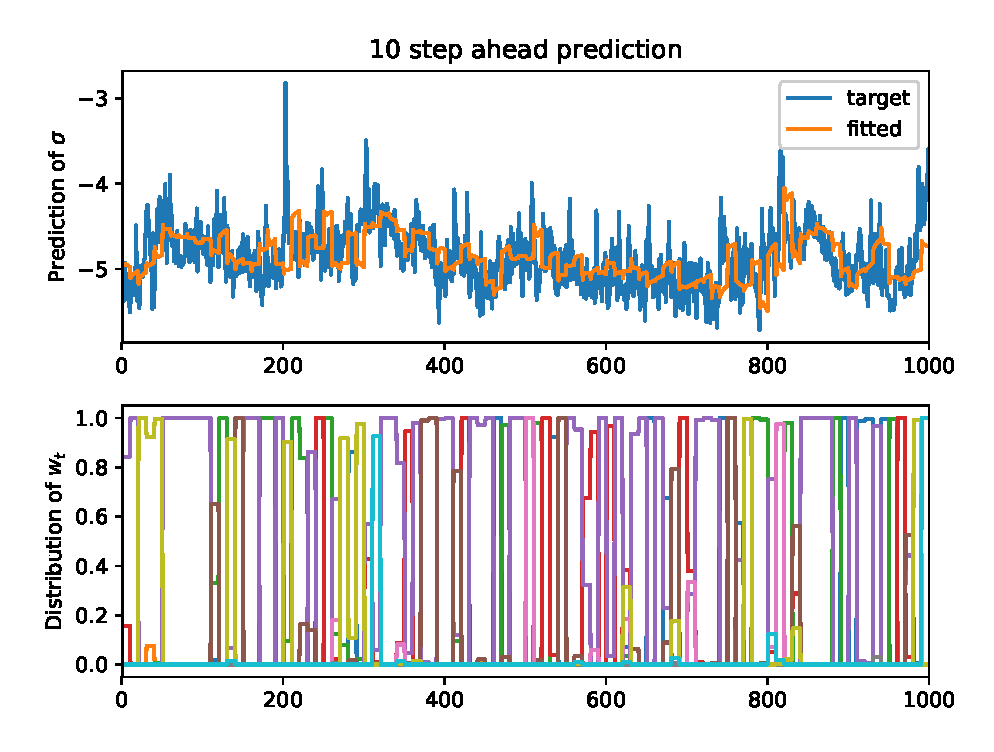
\includegraphics[width=0.45\textwidth]{Plots/Prediction/Plasticity_Constant_10step.eps}
    \end{center}
    \caption{This presents the predictive performance of the \textit{plasticity experts} for 1, 2, 5 and 10 step ahead predictions. The targeted network activations are using a constant $\sigma = \frac{1}{\sqrt{2\pi}}$ for all networks. The networks have only been trained once on the training set as outlined in section \ref{CH:Application:Forecasting:Fixed}.}
    \label{FIG:PlasticityConstant}
\end{figure}

\begin{figure}
    \begin{center}
        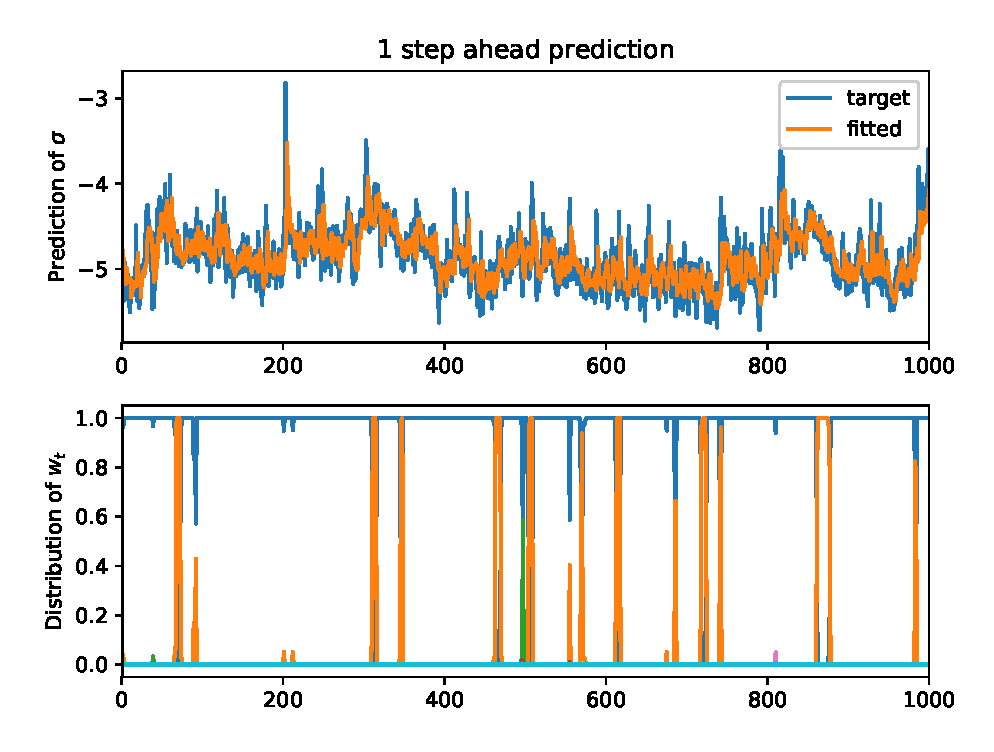
\includegraphics[width=0.45\textwidth]{Plots/Prediction/Plasticity_Grid_1step.eps}
        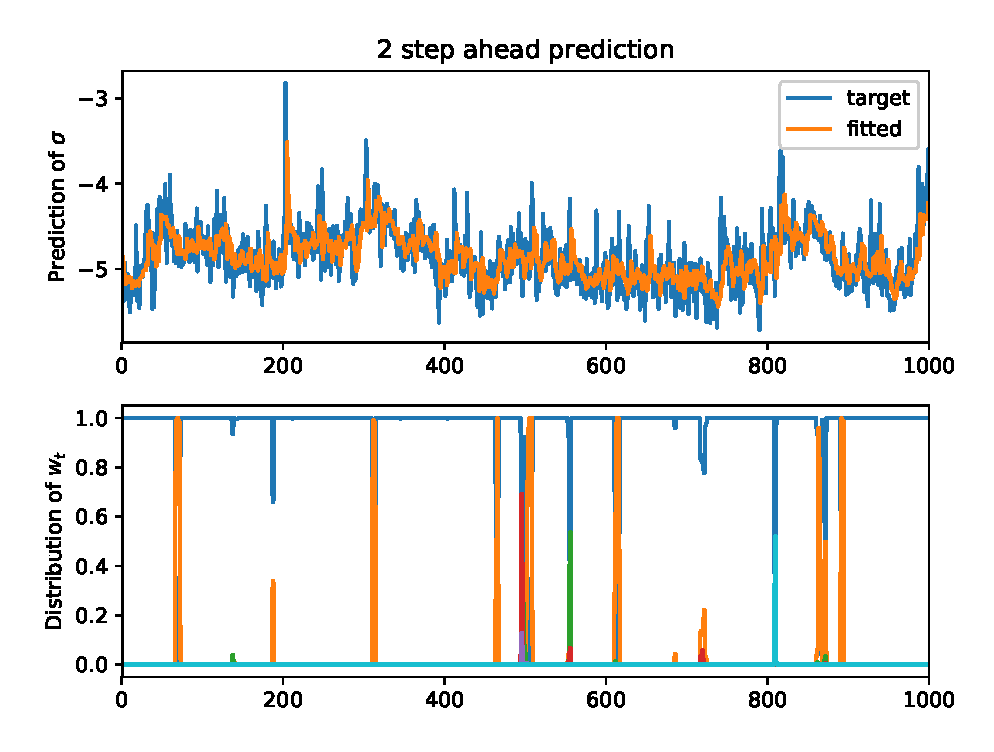
\includegraphics[width=0.45\textwidth]{Plots/Prediction/Plasticity_Grid_2step.eps} \\
        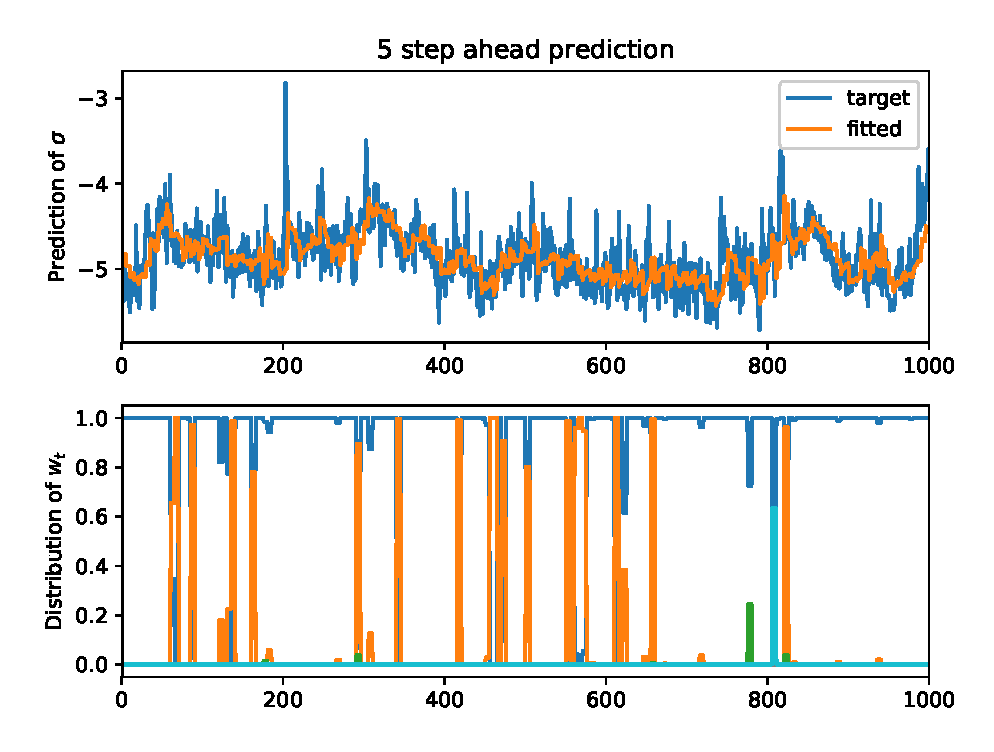
\includegraphics[width=0.45\textwidth]{Plots/Prediction/Plasticity_Grid_5step.eps}
        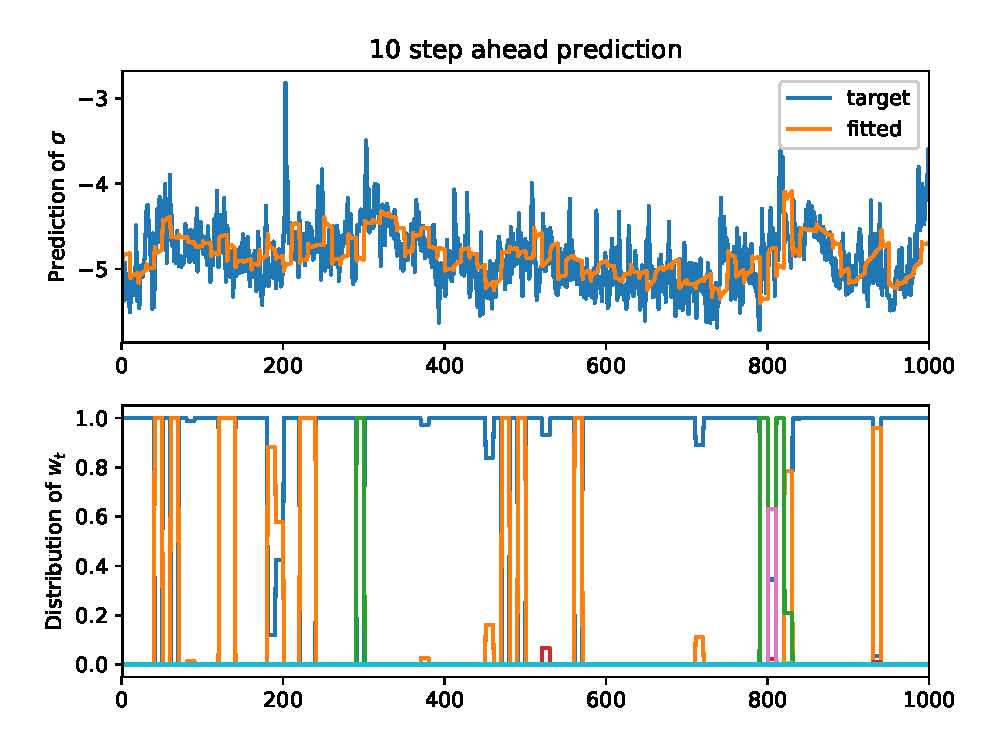
\includegraphics[width=0.45\textwidth]{Plots/Prediction/Plasticity_Grid_10step.eps} \\
        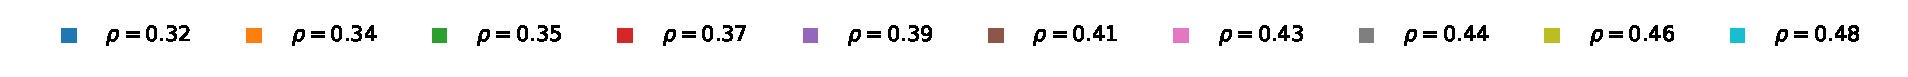
\includegraphics[width=1.0\textwidth]{Plots/Prediction/legend_Grid.eps}
        \label{FIG:PlasticityGrid}
    \end{center}
    \caption{This presents the predictive performance of the \textit{plasticity experts} for 1, 2, 5 and 10 step ahead predictions. The targeted network activations are using an equally spaced grid $\left[0.8\frac{1}{\sqrt{2\pi}}, 1.2\frac{1}{\sqrt{2\pi}}\right]$ around the constant value of $\sigma = \frac{1}{\sqrt{2\pi}}$. The networks have only been trained once on the training set as outlined in section \ref{CH:Application:Forecasting:Fixed}.}
\end{figure}

\begin{figure}
    \begin{center}
        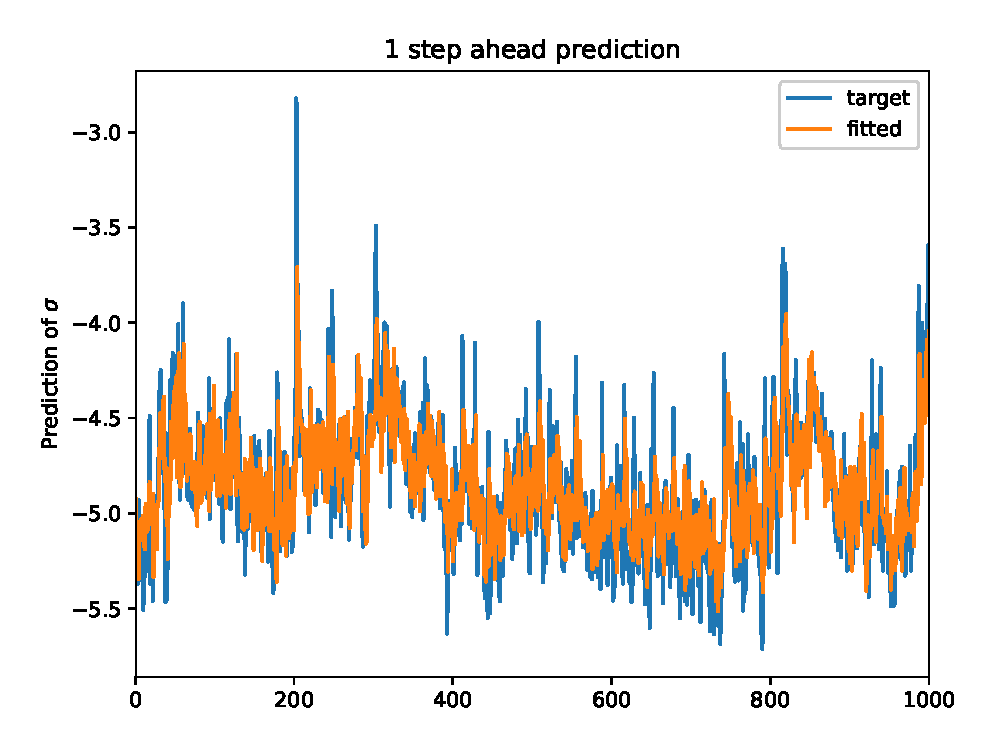
\includegraphics[width=0.45\textwidth]{Plots/Prediction/Single_logMSE_1step.eps}
        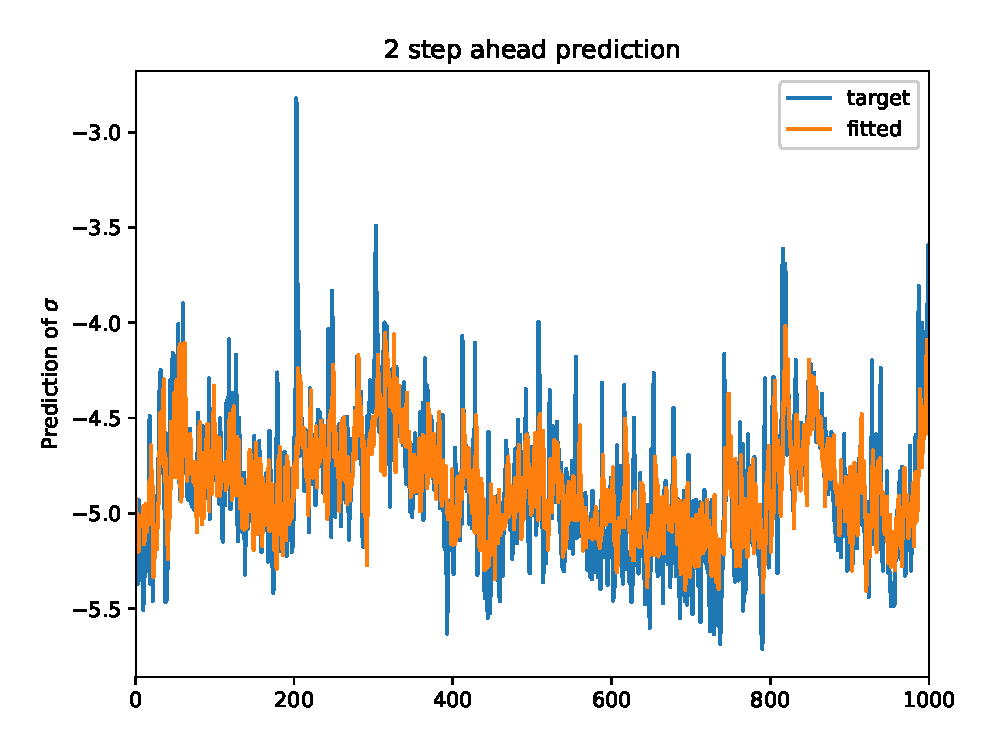
\includegraphics[width=0.45\textwidth]{Plots/Prediction/Single_logMSE_2step.eps} \\
        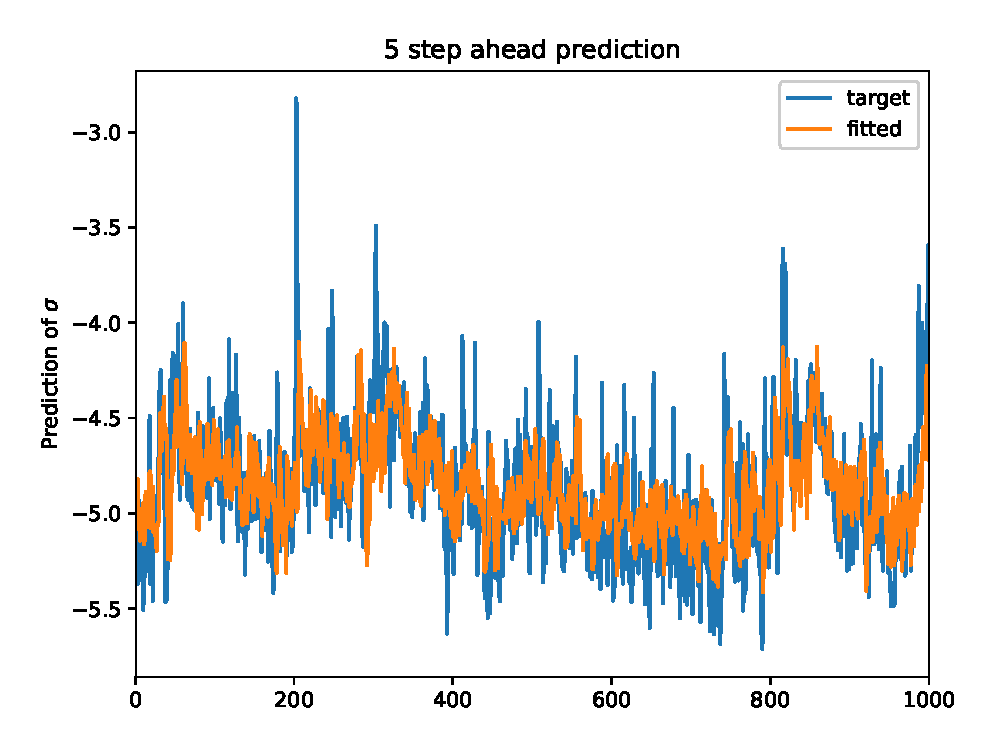
\includegraphics[width=0.45\textwidth]{Plots/Prediction/Single_logMSE_5step.eps}
        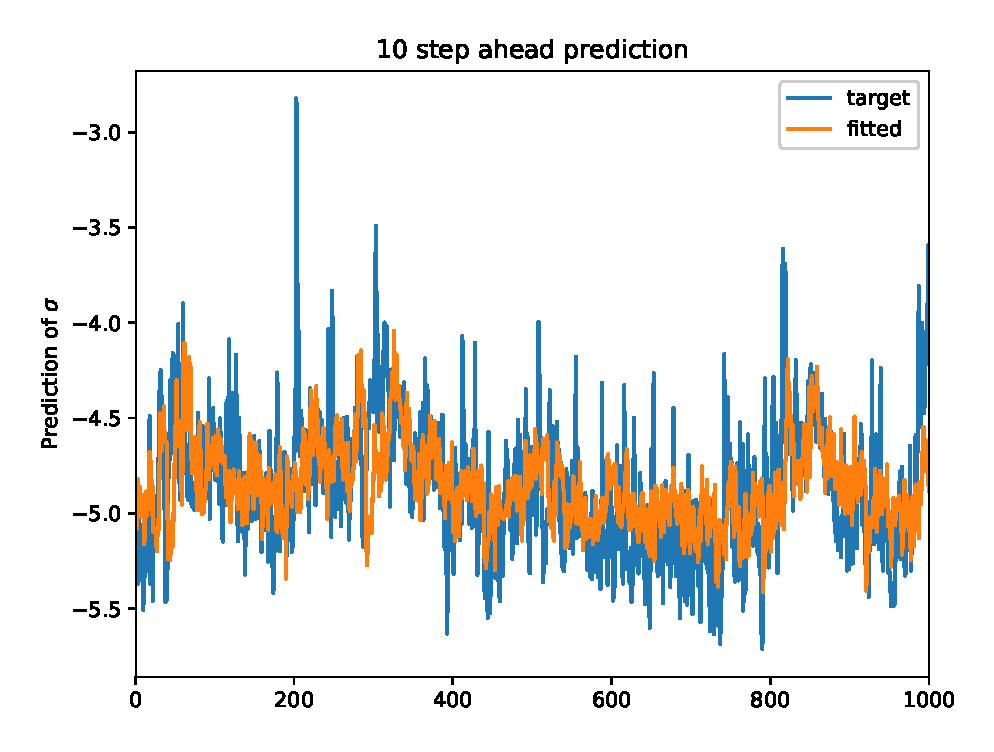
\includegraphics[width=0.45\textwidth]{Plots/Prediction/Single_logMSE_10step.eps}
        \label{FIG:SingleESN}
    \end{center}
    \caption{Single Echo State Network of equivalent size to the experts approach, namely $N=1000$ internal neurons. The hyperparameters that have been tuned for the logMSE are the spectral radius and the bias in the interval $\rho \in (0, 3]$ and bias $b \in [-1,1]$ and using a gradient boosted regression tree from the scikit-optimize package. See the appendix for details on this package.}
\end{figure}


\begin{figure}
    \begin{center}
        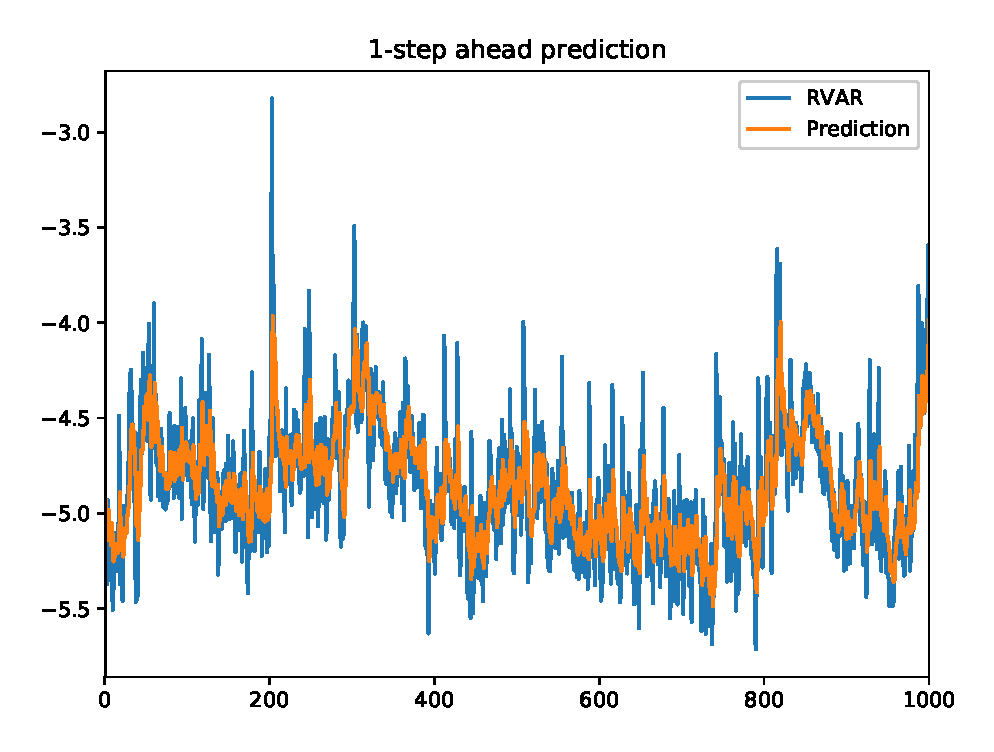
\includegraphics[width=0.45\textwidth]{Plots/Prediction/HAR_1step.eps}
        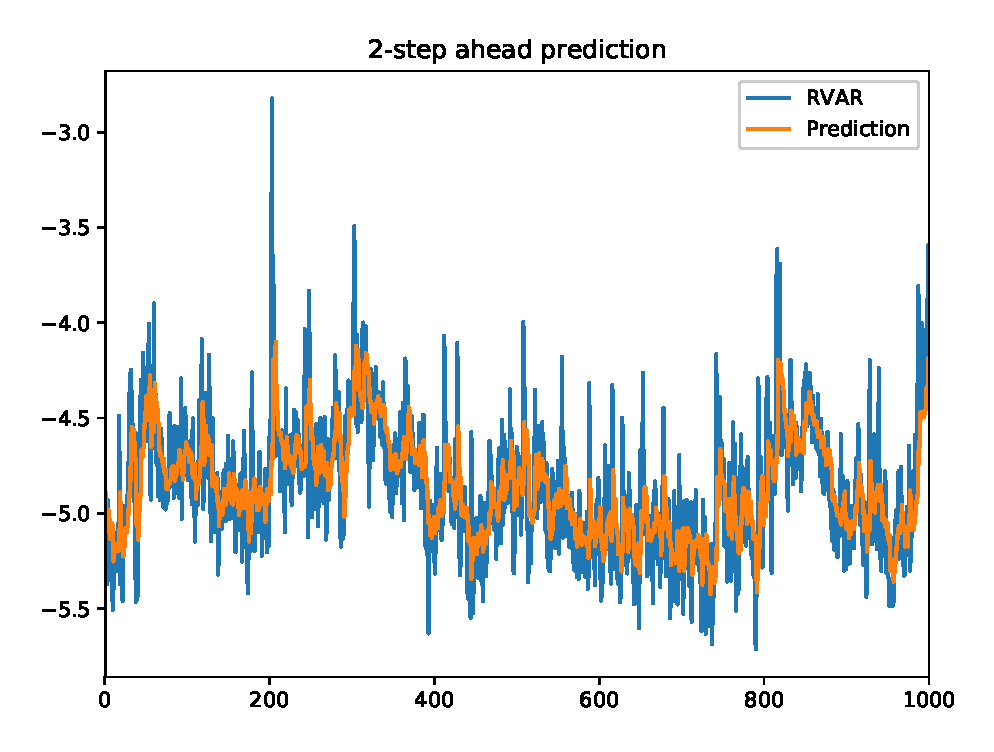
\includegraphics[width=0.45\textwidth]{Plots/Prediction/HAR_2step.eps} \\
        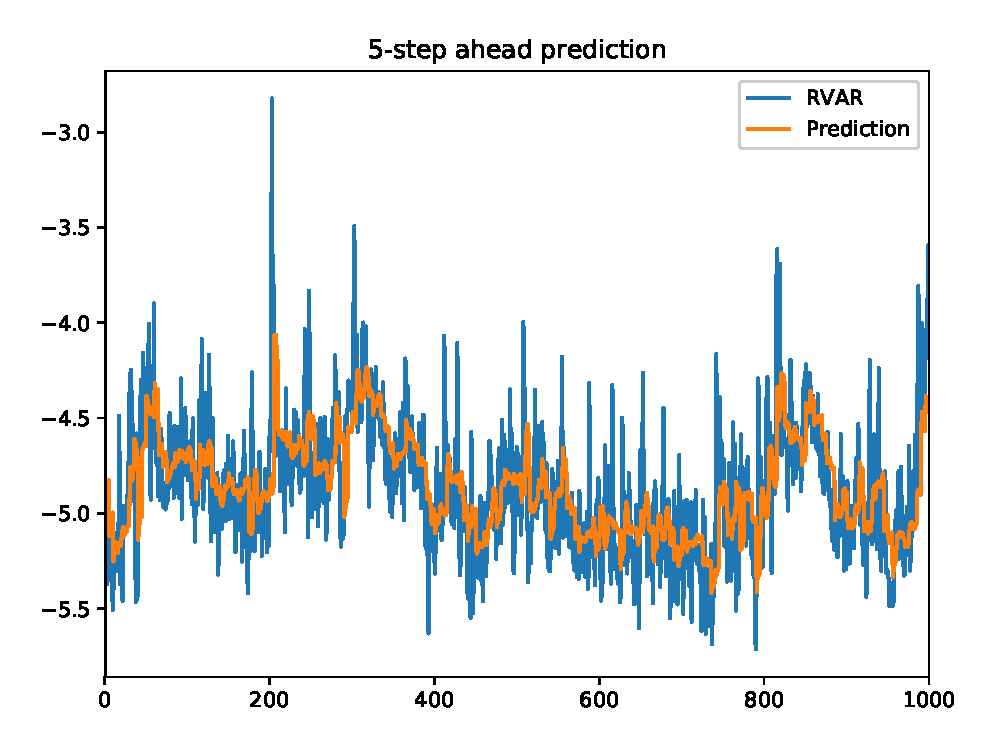
\includegraphics[width=0.45\textwidth]{Plots/Prediction/HAR_5step.eps}
        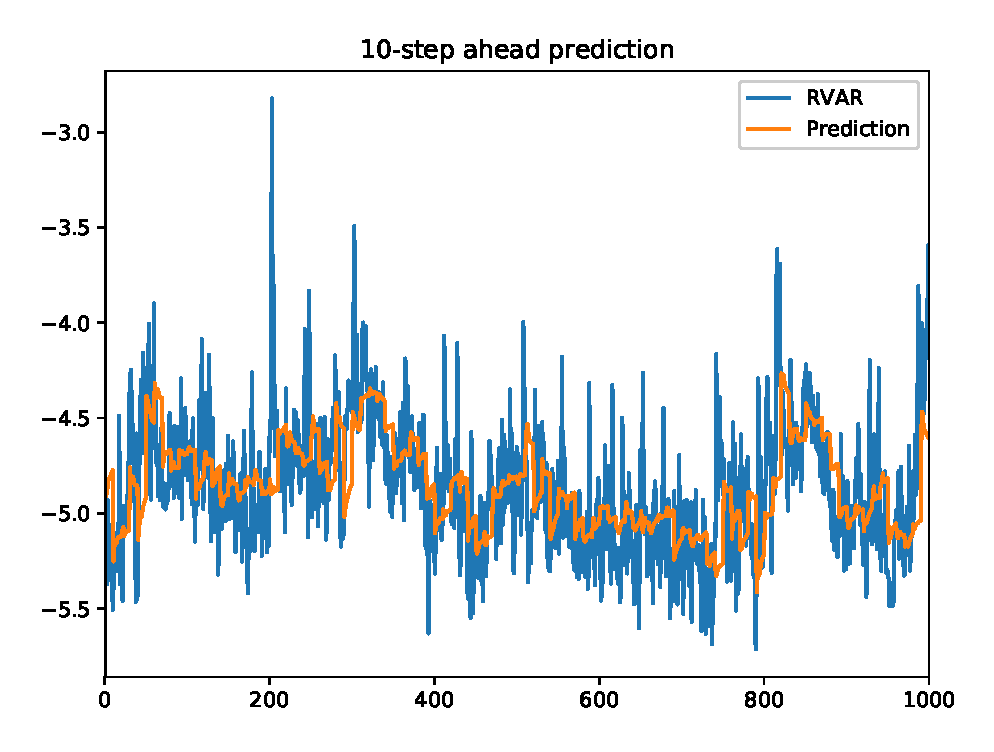
\includegraphics[width=0.45\textwidth]{Plots/Prediction/HAR_10step.eps}
    \end{center}
    \caption{HAR model as proposed by \cite{Corsi2009}, e.g. with daily, weekly and monthly realized volatilities, that has been trained in an online fashion along the lines of recursive least squares \refp{EQ:RLS21}-\refp{EQ:RLS22}.}
    \label{FIG:HAR}
\end{figure}



The figures \ref{FIG:ExpertsLogMSE} to \ref{FIG:HAR} present the predictiven performance of the different models and, in case of the expert methods, the distribution of their weightings over the course of the out-of-sample prediction horizon.
The \textit{loss experts} show a very consistent behaviour for all the error measurements in regards of their weights distribution. There are minor differences but the overall picture of the evolution of the weights stays the same for all apporaches which comes back to the fact that the underlying networks are the same because we fixed the random number generator. Additionally, because the Mean Square Error approach to the weighting showed very little movement when only using equation \refp{EQ:LossUpdate}, the errors for all models were rescaled to $[0,1]$ before applying equation \refp{EQ:LossUpdate} to keep the comparison between the models.
The 1-step ahead prediction is very volatile in terms of the weights which decreases with an increase in the prediction horizon. One can clearly see the dominance of the network with $\rho= 0.2$ in the period from step $500$ to time step $800$ where the series is trending down with little volatility. In the 2-step prediction, the network with the smallest spectral radius of $0.2$ dominates towards the end of the out-of-sample period which is not expected given that the increase in the prediction step would be expected to favor networks with longer memory, so a higher spectral radius. The network with $\rho = 2.0$ is dominating in the mid to end section of the horizon after $\rho = 0.8$ and $\rho = 1.2$ have taken over after $\rho = 0.4$ started the out-of-sample prediction. The weights assigned to networks with smaller spectral radii could be explained by the fact, that the output connections $\wout$ of the networks have not been retrained during the out-ouf-sample prediction and this may be indicative of a regime shift, where the long term dependencies in the series have changed and the prediction is predominantly based on the recent history of the series. On the contrary, there are the 5-step and 10-step ahead predictions. There the networks with the largest spectral radius of $\rho = 2.0$ as gaining weight in the 5-step prediction and and is clearly dominating the 10-step prediction which means that the longer term dependencies are a dominant factor for the predictive ability. Looking at the \textit{loss experts} in figure \ref{FIG:ExpertsMSE} the MSE in the original scale as loss function, the 1-step ahead prediction is still very volatile. The 2-step ahead prediction also shows a very similar picture except that the network with $\rho = 2.0$ is not gaining as much weight as in the log-scale MSE case. The 5-step and 10-step prediction differ significantly. For the original-scale MSE the networks with the lowest spectral radii of $\rho = 0.4$ and $\rho = 0.2$ receive the dominant weights in the beginning and end section of the prediction horizon, respectively.
The QLIKE weighted experts in figure \ref{FIG:ExpertsQLIKE} show a combination of the previous two weighting approaches. Where, still, the 1-step ahead prediction shows its volatile and very similar picture, the 2-step ahead prediction resembles the log-scale MSE distribution of weights and the 5-step and 10-step prediction are more similar to the original-scale MSE weighted experts. The 10-step prediction is even more extrem in the sense, that the network with $\rho = 0.4$ receives a weight of $1$ almost all of the time.

The \textit{plasticity experts} with the same output distributions in figure \ref{FIG:PlasticityConstant} do present a very volatile and quickly adapting behaviour. The similarity between the four panels of figure \ref{FIG:PlasticityConstant} is expected given that after the prediction, the network evolution is corrected by the true series and this is done for all prediction steps. The only difference is the granularity of the weights update which can be seen very well comparing the 1-step and 10-step ahead prediction. The latter behaves like a step function. Additionally, comparing the weights to the experts approach, the distribution of component weights is much more extrem in the sense that the weights mostly alternate between $0$ and $1$ and in rare occasions have a true mixture of components. The similarity of all the panels leads to the conclusion that the empirical distribution and the resulting likelihood of a network's activation can change very quickly. The series and the distribution of the weights, unfortunately, don't seem to correspond in a certain way.
The \textit{plasticity experts} with a grid of output distributions in figure \ref{FIG:PlasticityGrid} on the other hand do present a very different distribution of output weights. Where with constant distributions, most of the networks were involved in the prediction at one point in time, the two experts with the lowest volatility distributions of $\sigma = 0.32$ and $\sigma = 0.34$ make up the resulting predictions. As with the constant plasticity experts the weights alternate between $0$ and $1$ and don't seem to coincide with the series in any remarkable pattern. In very few instances, the networks with $\sigma = 0.35$ and $\sigma = 0.37$ do receive a small weight which is not of long duration\footnote{The values for $\sigma$ don't seem equidistant but this is due to the rounding to two digits.}.

Plots for the predictive performance of the single ESN and the HAR model are provided in figures \ref{FIG:SingleESN} and \ref{FIG:HAR}. The single ESN shows some very choppy behaviour which could indicate an overfitting during the training process. The tuned hyperparemeters of the single ESN are $\rho = 1.2511$ and $b = 0.4406$ \footnote{The bias $b$ is multiplied by $\wbias$ to become $\bb = b \cdot \wbias$.}. The HAR model is in line with expectations. The difference can also be attributed to the fact that the predictions are plotted in the log-scale of $\sigma$. The higher the prediction steps, the calmer the predictions become. Where in the panel of 1-step ahead predictions the forecasts do follow the true series quite strongly this effect decreases with the prediction step and the forecasts have a tendency towards the histrical mean of the series.

For the single ESN, only the prediction of the logMSE related measurements are presented because the chosen hyperparameters were almost the same as the other two error measurements. Out of the three, the logMSE was chosen as it is related to the original scale of the series, namely $\sigma$. The very volatile behaviour of the predictions leads to the concern of overfitting during the training of the network's output connections. This is supported by the fact that the regularization parameter of the ridge regression was chosen on the border of admissible values.

\begin{table}
    \begin{center}
        
\begin{tabular}{l|c|c|c}
Fixed 1-step ahead     & logMSE & MSE $(\times 10^{-5})$ & QLIKE \\\hline
Experts MSE & 0.08758738 & 1.05803697 & 0.24808956\\ 
Experts QLIKE & 0.08760709 & 1.05505096 & 0.24823963\\ 
Experts logMSE & 0.08758126 & 1.05689476 & 0.24847465\\ 
HAR & 0.06847035 & 0.84973355 & 0.19371920\\ 
Plasticity Constant & 0.08933186 & 1.04572311 & 0.25836014\\ 
Plasticity Grid & 0.08640221 & 1.01276597 & 0.25078255\\ 
Single MSE & 0.08334474 & 0.94009009 & 0.20983467\\ 
Single QLIKE & 0.07926708 & 0.93331580 & 0.20988650\\ 
Single logMSE & 0.08267177 & 0.95702170 & 0.22700093\\ 
\end{tabular}
    \end{center}
    \caption{Errors for the prediction for the different models and the $1$-step ahead predictions using a fixed training set as outlined in section \ref{CH:Application:Forecasting:Fixed}.}
    \label{TABLE:1step}
\end{table} 

\begin{table}
    \begin{center}
        
\begin{tabular}{l|c|c|c}
Fixed 2-step ahead     & logMSE & MSE $(\times 10^{-5})$ & QLIKE \\\hline
Experts MSE & 0.08986521 & 1.07277764 & 0.25348541\\ 
Experts QLIKE & 0.09085416 & 1.09143206 & 0.25588969\\ 
Experts logMSE & 0.09084808 & 1.08410217 & 0.25612836\\ 
HAR & 0.07503286 & 0.91231669 & 0.21128034\\ 
Plasticity Constant & 0.08938321 & 1.05612199 & 0.26294063\\ 
Plasticity Grid & 0.08817040 & 1.03261120 & 0.25984234\\ 
Single MSE & 0.08974965 & 1.00270113 & 0.22271637\\ 
Single QLIKE & 0.08679926 & 0.99016069 & 0.23042241\\ 
Single logMSE & 0.09181919 & 1.04655279 & 0.25124330\\ 
\end{tabular}
    \end{center}
    \caption{Errors for the prediction for the different models and the $2$-step ahead predictions using a fixed training set as outlined in section \ref{CH:Application:Forecasting:Fixed}..}
    \label{TABLE:2step}
\end{table}

\begin{table}
    \begin{center}
        
\begin{tabular}{l|c|c|c}
Fixed 5-step ahead     & logMSE & MSE $(\times 10^{-5})$ & QLIKE \\\hline
Experts MSE & 0.09987065 & 1.17159711 & 0.30540002\\ 
Experts QLIKE & 0.09973242 & 1.16626035 & 0.30564940\\ 
Experts logMSE & 0.09832657 & 1.14407191 & 0.30210400\\ 
HAR & 0.08737418 & 1.03945024 & 0.26712508\\ 
Plasticity Constant & 0.09897247 & 1.14413505 & 0.31834281\\ 
Plasticity Grid & 0.09600595 & 1.11135717 & 0.31021388\\ 
Single MSE & 0.10656475 & 1.19625577 & 0.29094670\\ 
Single QLIKE & 0.09785688 & 1.11072290 & 0.28079199\\ 
Single logMSE & 0.10401672 & 1.16531048 & 0.30932509\\ 
\end{tabular}
    \end{center}
    \caption{Errors for the prediction for the different models and the $5$-step ahead predictions using a fixed training set as outlined in section \ref{CH:Application:Forecasting:Fixed}..}
    \label{TABLE:5step}
\end{table}

\begin{table}
    \begin{center}
        
\begin{tabular}{l|c|c|c}
Fixed 10-step ahead     & logMSE & MSE $(\times 10^{-5})$ & QLIKE \\\hline
Experts MSE & 0.10915740 & 1.25883661 & 0.33336069\\ 
Experts QLIKE & 0.11004703 & 1.25491580 & 0.34062729\\ 
Experts logMSE & 0.11021187 & 1.24497983 & 0.33841503\\ 
HAR & 0.10138104 & 1.16342703 & 0.31118643\\ 
Plasticity Constant & 0.11787165 & 1.31586371 & 0.36889776\\ 
Plasticity Grid & 0.11188359 & 1.25658633 & 0.34886447\\ 
Single MSE & 0.12216529 & 1.31975650 & 0.34693690\\ 
Single QLIKE & 0.11271315 & 1.23937364 & 0.32947925\\ 
Single logMSE & 0.11743093 & 1.31681358 & 0.35623439\\ 
\end{tabular}
    \end{center}
    \caption{Errors for the prediction for the different models and the $10$-step ahead predictions using a fixed training set as outlined in section \ref{CH:Application:Forecasting:Fixed}..}
    \label{TABLE:10step}
\end{table}


The tables \ref{TABLE:1step} to \ref{TABLE:10step} present the prediction error for the out-of-sample part of the series, this is the last $1000$ observations, for the different prediction step sizes. 
The error measurements, namely logMSE, MSE and QLIKE are referring to the different scales of $\log{\sigma}$, $\sigma$ and $\sigma^2$, respectively, which is in accordance with the hyperparameters' validation of the \textit{loss experts} and the single ESN.

The HAR model by \cite{Corsi2009} presents the best performance throughout all prediction steps for the logMSE. After the log transformation the volatility process becomes linear and it is to be exptected that the HAR model, which can be regarded as a restricted AR(22) model and therefore is linear, should outperform the other models in this matter. The better performance of the HAR model can also be seen in MSE and in the QLIKE error. This phenomenon can be explained by the fact that the HAR model is by its nature of an AR-process capturing changes in the regime of the time series where the reservoir computing models are only fed the time series itself and don't receive a preprocessed (in the sense of aggregation) of the signal. The only regime change that the HAR model is not able to adapt to is the intercept, but this is also the case for the other models and in comparison the HAR model beats all other models. This will also become clearer in the following section \ref{CH:EmpiricalResults:Rolling}

Comparing the \textit{plasticity experts} and the \textit{loss experts} in the logMSE, the predictive performance of the former is better for the $1$, $2$ and $5$-step ahead prediction and also for the $10$ step prediction when using the grid of targeted output distributions. The $10$-step ahead prediction horizon of the constant plasticities is worse compared to the experts of all loss functions. This tendency mostly continues for the MSE, where the \textit{plasticity experts} outperform the \textit{loss experts} up to the $5$-step prediction but both \textit{plasticity experts}, with constant output distributions and using a grid, are not able to beat the \textit{loss experts} in the MSE.

A comparison between the two plasticity approaches is difficult as the the constant distribution seems to outperform in the logMSE and the MSE for the $5$ and $10$-step prediction, but the grid of distributions seems to be favourable in terms of logMSE and QLIKE for the $1$ and $2$-step prediction setting.

The \textit{loss experts} consistently dominate in the QLIKE where, independent of the prediction step, they outperform all other model specifications.

\subsubsection{Rolling Training Performance}
\label{CH:EmpiricalResults:Rolling}

This section presents the out-of-sample performance for the approach where the training set is shifted into the testing set. This procedure has been outlined in section \ref{CH:Application:Forecasting:Rolling}.


\begin{figure}
    \begin{center}
        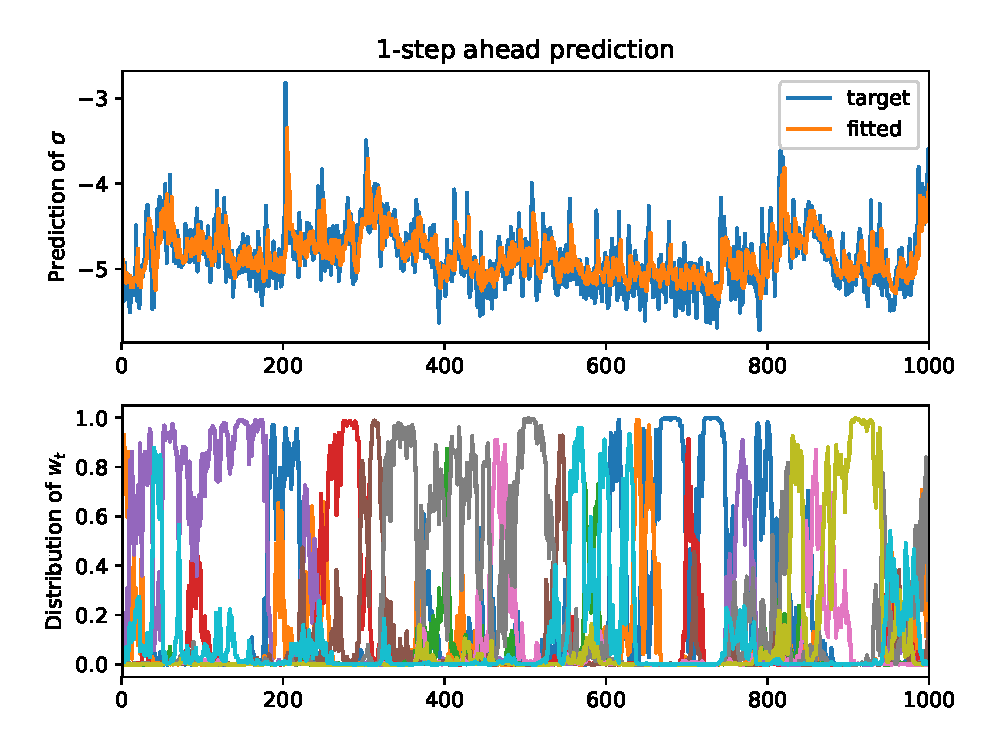
\includegraphics[width=0.45\textwidth]{Plots/Prediction/Experts_logMSE_rolling_1step.eps}
        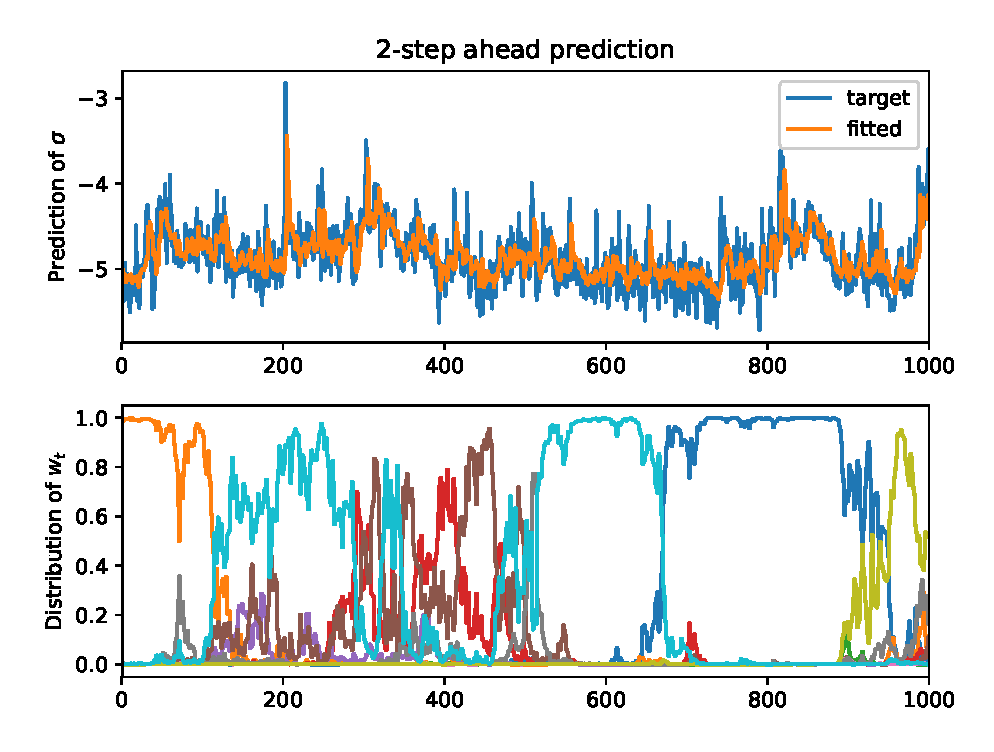
\includegraphics[width=0.45\textwidth]{Plots/Prediction/Experts_logMSE_rolling_2step.eps} \\
        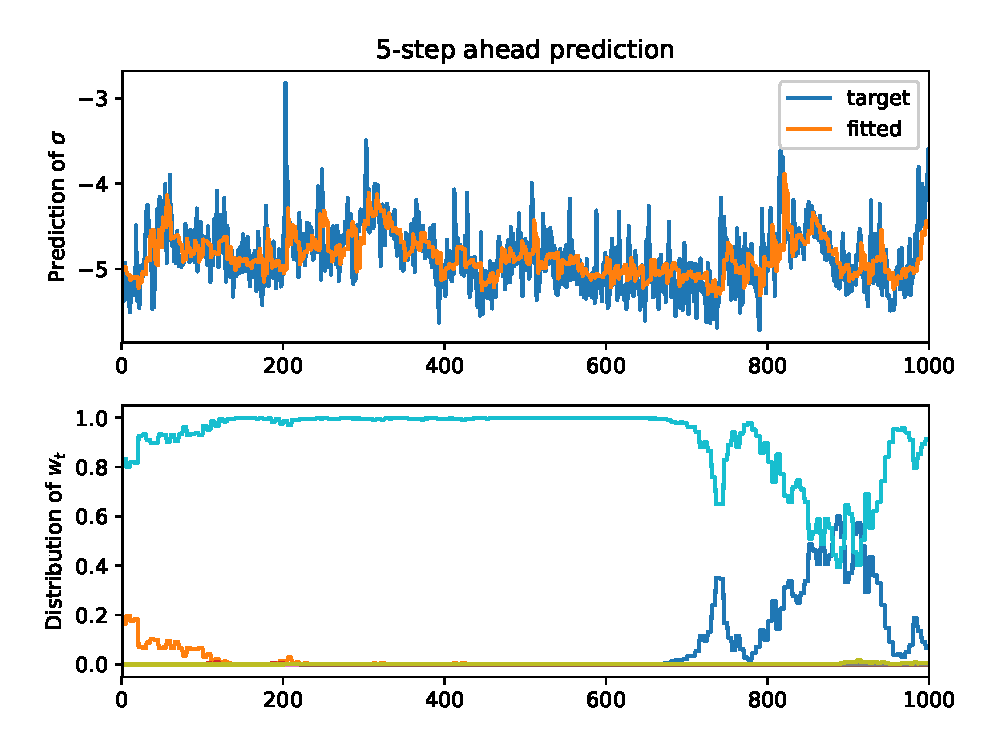
\includegraphics[width=0.45\textwidth]{Plots/Prediction/Experts_logMSE_rolling_5step.eps}
        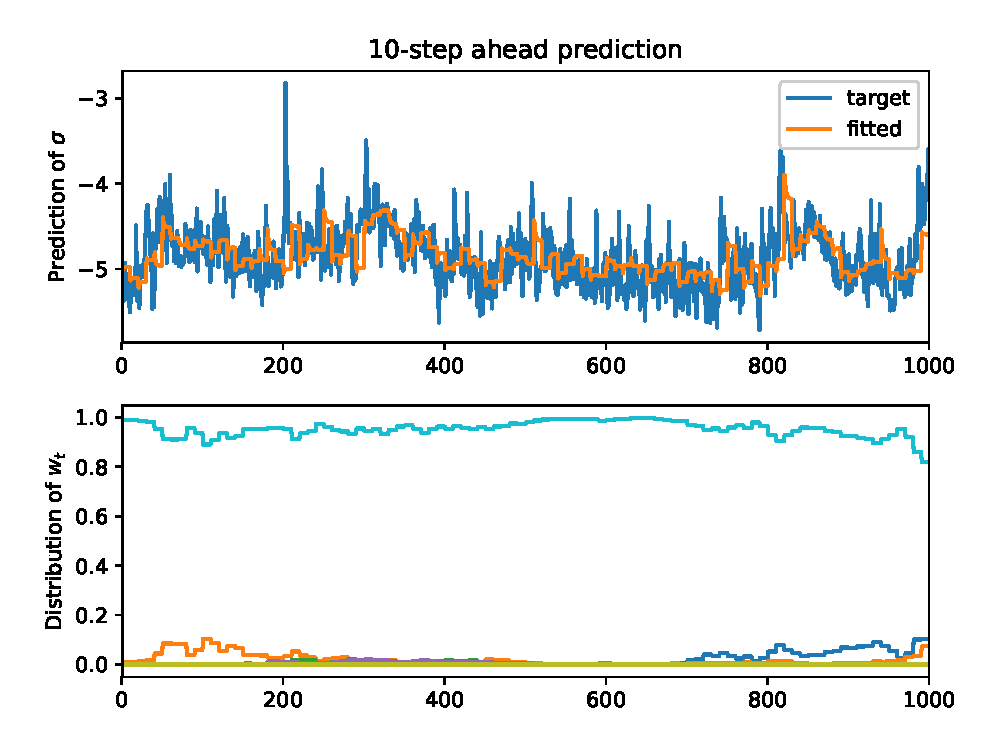
\includegraphics[width=0.45\textwidth]{Plots/Prediction/Experts_logMSE_rolling_10step.eps} \\
        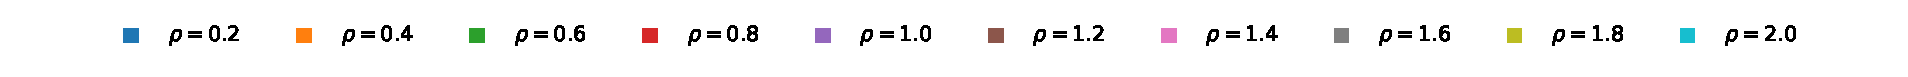
\includegraphics[width=1.0\textwidth]{Plots/Prediction/legend_experts.eps}
        \label{FIG:ExpertsLogMSERolling}
    \end{center}
    \caption{This is the \textit{loss experts} approach with exponential weighting of the experts based on the mean squared error of the log transformation $\log{\sigma}$. The values of spectral radii are equally space in the interval $\rho \in [0.2, 2.0]$. The networks have been retrained in a rolling window fashion as outlined in section \ref{CH:Application:Forecasting:Rolling}.}
\end{figure}

\begin{figure}
    \begin{center}
        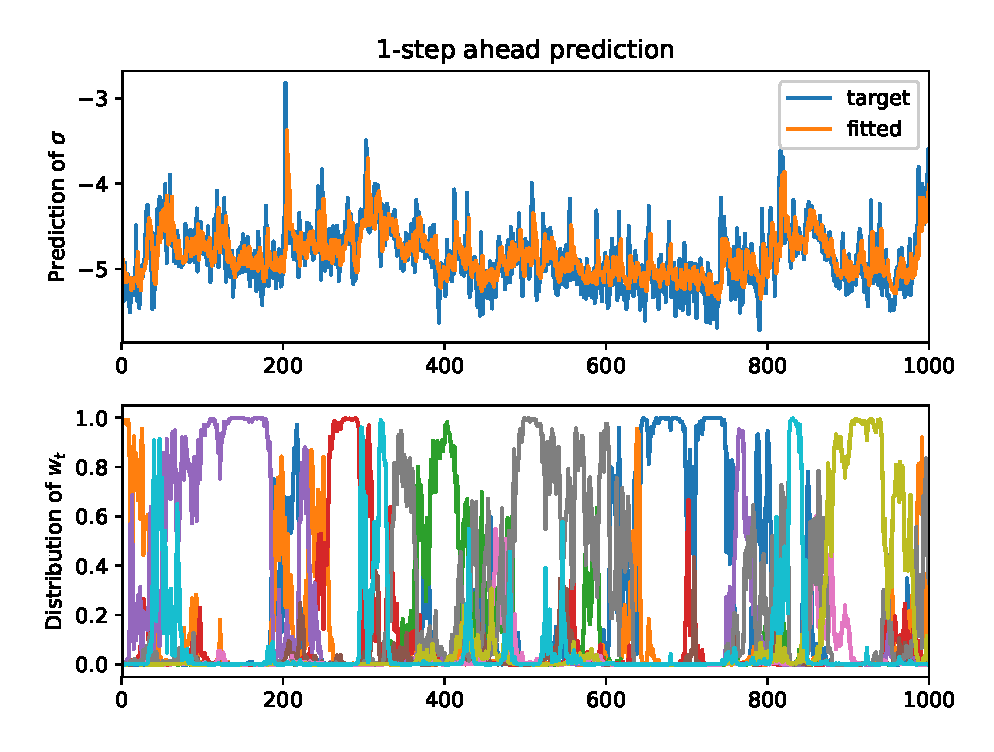
\includegraphics[width=0.45\textwidth]{Plots/Prediction/Experts_MSE_rolling_1step.eps}
        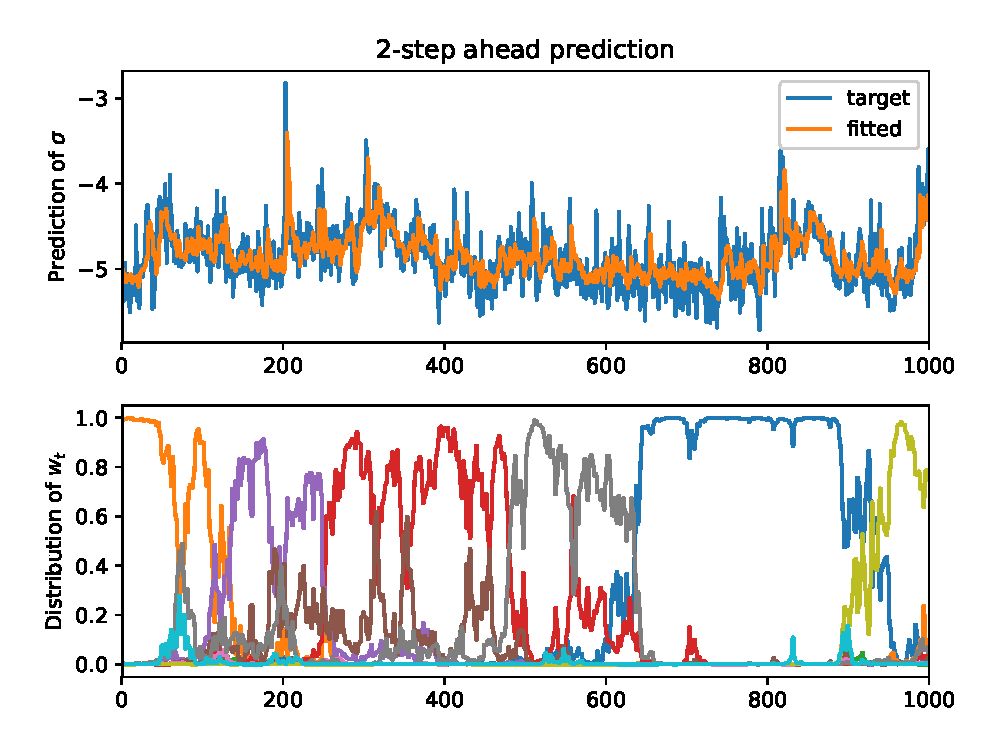
\includegraphics[width=0.45\textwidth]{Plots/Prediction/Experts_MSE_rolling_2step.eps} \\
        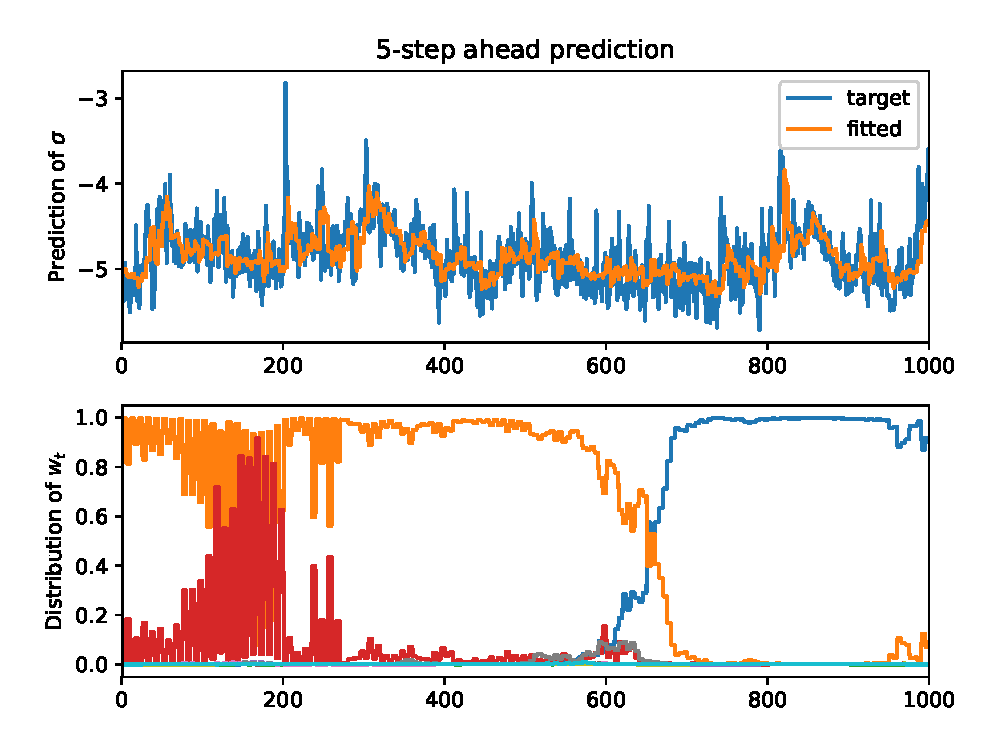
\includegraphics[width=0.45\textwidth]{Plots/Prediction/Experts_MSE_rolling_5step.eps}
        \includegraphics[width=0.45\textwidth]{Plots/Prediction/Experts_MSE_rolling_10step.eps} \\
        \includegraphics[width=1.0\textwidth]{Plots/Prediction/legend_experts.eps}
    \end{center}
    \caption{This is the \textit{loss experts} approach with exponential weighting of the experts based on the mean squared error of the original time series, so $\sigma$. The values of spectral radii are equally space in the interval $\rho \in [0.2, 2.0]$. The networks have been retrained in a rolling window fashion as outlined in section \ref{CH:Application:Forecasting:Rolling}.}
    \label{FIG:ExpertsMSERolling}
\end{figure}

\begin{figure}
    \begin{center}
        \includegraphics[width=0.45\textwidth]{Plots/Prediction/Experts_QLIKE_rolling_1step.eps}
        \includegraphics[width=0.45\textwidth]{Plots/Prediction/Experts_QLIKE_rolling_2step.eps} \\
        \includegraphics[width=0.45\textwidth]{Plots/Prediction/Experts_QLIKE_rolling_5step.eps}
        \includegraphics[width=0.45\textwidth]{Plots/Prediction/Experts_QLIKE_rolling_10step.eps} \\
        \includegraphics[width=1.0\textwidth]{Plots/Prediction/legend_experts.eps}
    \end{center}
    \caption{This is the \textit{loss experts} approach with exponential weighting of the experts based on the QLIKE loss function, so in the scale of $\sigma^2$. The values of spectral radii are equally space in the interval $\rho \in [0.2, 2.0]$. The networks have been retrained in a rolling window fashion as outlined in section \ref{CH:Application:Forecasting:Rolling}.}
    \label{FIG:ExpertsQLIKERolling}
\end{figure}


\begin{figure}
    \begin{center}
        \includegraphics[width=0.45\textwidth]{Plots/Prediction/Plasticity_Constant_rolling_1step.eps}
        \includegraphics[width=0.45\textwidth]{Plots/Prediction/Plasticity_Constant_rolling_2step.eps} \\
        \includegraphics[width=0.45\textwidth]{Plots/Prediction/Plasticity_Constant_rolling_5step.eps}
        \includegraphics[width=0.45\textwidth]{Plots/Prediction/Plasticity_Constant_rolling_10step.eps}
    \end{center}
    \caption{This presents the predictive performance of the \textit{plasticity experts} for 1, 2, 5 and 10 step ahead predictions. The targeted network activations are using a constant $\sigma = \frac{1}{\sqrt{2\pi}}$ for all networks. The networks have been retrained in a rolling window fashion as outlined in section \ref{CH:Application:Forecasting:Rolling}.}
    \label{FIG:PlasticityConstantRolling}
\end{figure}

\begin{figure}
    \begin{center}
        \includegraphics[width=0.45\textwidth]{Plots/Prediction/Plasticity_Grid_rolling_1step.eps}
        \includegraphics[width=0.45\textwidth]{Plots/Prediction/Plasticity_Grid_rolling_2step.eps} \\
        \includegraphics[width=0.45\textwidth]{Plots/Prediction/Plasticity_Grid_rolling_5step.eps}
        \includegraphics[width=0.45\textwidth]{Plots/Prediction/Plasticity_Grid_rolling_10step.eps} \\
        \includegraphics[width=1.0\textwidth]{Plots/Prediction/legend_Grid.eps}
    \end{center}
    \caption{This presents the predictive performance of the \textit{plasticity experts} for 1, 2, 5 and 10 step ahead predictions. The targeted network activations are using an equally spaced grid $\left[0.8\frac{1}{\sqrt{2\pi}}, 1.2\frac{1}{\sqrt{2\pi}}\right]$ around the constant value of $\sigma = \frac{1}{\sqrt{2\pi}}$. The networks have been retrained in a rolling window fashion as outlined in section \ref{CH:Application:Forecasting:Rolling}.}
    \label{FIG:PlasticityGridRolling}
\end{figure}

\begin{figure}
    \begin{center}
        \includegraphics[width=0.45\textwidth]{Plots/Prediction/Single_logMSE_rolling_1step.eps}
        \includegraphics[width=0.45\textwidth]{Plots/Prediction/Single_logMSE_rolling_2step.eps} \\
        \includegraphics[width=0.45\textwidth]{Plots/Prediction/Single_logMSE_rolling_5step.eps}
        \includegraphics[width=0.45\textwidth]{Plots/Prediction/Single_logMSE_rolling_10step.eps}
    \end{center}
    \caption{Single Echo State Network of equivalent size to the experts approach, namely $N=1000$ internal neurons. The hyperparameters that have been tuned for the logMSE are the spectral radius and the bias in the interval $\rho \in (0, 3]$ and bias $b \in [-1,1]$ and using a gradient boosted regression tree from the scikit-optimize package. See the appendix for details on this package. The networks have been retrained in a rolling window fashion as outlined in section \ref{CH:Application:Forecasting:Rolling} but hyperparameters have only been optimized on the fixed training set.}
    \label{FIG:SingleESNRolling}
\end{figure}


\begin{figure}
    \begin{center}
        \includegraphics[width=0.45\textwidth]{Plots/Prediction/HAR_rolling_1step.eps}
        \includegraphics[width=0.45\textwidth]{Plots/Prediction/HAR_rolling_2step.eps} \\
        \includegraphics[width=0.45\textwidth]{Plots/Prediction/HAR_rolling_5step.eps}
        \includegraphics[width=0.45\textwidth]{Plots/Prediction/HAR_rolling_10step.eps}
    \end{center}
    \caption{HAR model as proposed by \cite{Corsi2009}, e.g. with daily, weekly and monthly realized volatilities. In line with the Echo State Networks, the HAR model has been retrained in the same rolling window fashion as the reservoir commputing models. Given the size of the dataset, no hyperparameters (e.g. regularization) were needed.}
    \label{FIG:HARRolling}
\end{figure}

Figures \ref{FIG:ExpertsLogMSERolling} to \ref{FIG:ExpertsQLIKERolling} present the performance of the performance of the \textit{loss experts} using the rolling window training. The logMSE trained networks shows a very consistent picture. The weighting in the 1-step ahead predictions is very volatile where almost every network receives significant weight at some point over the testing horizon which leads to the interpretation that those predictions are an interplay of short term moves (smaller $\rho$) and longer term trends (higher $\rho$). In the 2-step head prediction, the weights are not as widely distributed over the networks but mostly assigned to the networks with $\rho = 0.4$ in the very beginning, followed by $\rho = 2.0$ towards the middle and $\rho = 0.2$ dominating the end section of the horizon. $\rho = 1.8$ gains some weight in the very end. The 5-step and 10-step ahead predictions present a clear dominance of $\rho = 2.0$ over most of the horizon for the 5-step and over the whole horizon for the 10-step predictions. This is in line with expectations because a higher $\rho$ signifies a longer memory of the network which is needed for longer out-of-sample predictions.

The broad picture of the weights' distribution is the same for the 1-step and 2-step ahead prediction in the \textit{loss experts} with the MSE as error function. The 1-step ahead prediction shows a very similar picture, but slight differences are recognizable by just eyeballing. The 2-step ahead prediction as well shows a very similar picture, however, the weight of $\rho = 2.0$ that is present in the logMSE seems to have been replaced by the network with $\rho = 1.0$ that gains some weight in the beginning to mid section of the prediction.

Putting the \textit{loss experts} with the QLIKE loss function in contrast with the other two, the results look more in line with the MSE than with the logMSE experts. This makes sense because the scales of $\sigma$ and $\sigma^2$ are more alike compared to the $\log{\sigma}$. Surprisingly, the 1-step and 2-step ahead prediction, as with the MSE, still look similar in the sense, that we find a broad spectrum of networks receiving weight in the 1-step ahead prediction and for the 2-step ahead prediction the networks of $\rho = 0.4$, followed by a mixture of different networks, the network of $\rho = 0.2$ in the end section and $\rho = 1.8$ in the very end of the prediction horizon.
For the 5-step ahead prediction, the network with $\rho = 0.4$ is dominating in the beginning and towards the end, the network with $\rho = 0.2$ is taking over. They again switch roles in the very and it ends with $\rho = 0.4$ as the dominant network. The 10-step ahead prediction is dominated by $\rho = 0.4$ throughout the whole prediction horizon.

The general picture that we have seen in the \textit{loss experts} using MSE and QLIKE suggest that, if we are not in the log-scale, short term moves dominate the predictions of future volatility, which stands in contrast to the logMSE where the network with the highest value of $\rho$, namely the network with $\rho = 2.0$ tended to dominate the longer prediction horizons.


The \textit{plasticity experts} with equal output distributions show a very similar weight distribution compared to the fixed training set. The distribution is still very volatile which makes a direct comparison difficult. 
For the networks with different output distributions, however, the distribution is even more concentrated towards the network with $\sigma = 0.32$. This is the case for all prediction steps. While the network with the second lowest $\sigma = 0.34$ is sporadically and for very short amounts of time gaining some weight in the 1-step ahead prediction, this happens fewer and fewer as the prediction horizon increases. This doesn't seem to coincide with the series at all.
Tests with a different grid of lower values was performed as well but didn't show significant improvements in performance or further insights into the resulting weighting. Analyses are provided in appendix \ref{CH:Appendix:GridSmallerSigma}.

For the HAR model in figure \ref{FIG:HARRolling} we can see a very similar behaviour compared to the fixed training set of figure \ref{FIG:HAR}.




\begin{table}
    \begin{center}
        
\begin{tabular}{l|c|c|c}
Rolling 1-step ahead     & logMSE & MSE $(\times 10^{-5})$ & QLIKE \\\hline
Experts MSE & 0.08802286 & 1.06410393 & 0.24888490\\ 
Experts QLIKE & 0.08808350 & 1.06756442 & 0.24892281\\ 
Experts logMSE & 0.08813920 & 1.06925160 & 0.24909907\\ 
HAR & 0.06836762 & 0.84943039 & 0.19290737\\ 
Plasticity Constant & 0.08742805 & 1.03377312 & 0.25916568\\ 
Plasticity Grid & 0.08620444 & 1.02328620 & 0.25938944\\ 
Single MSE & 0.04375821 & 0.52195032 & 0.09560064\\ 
Single QLIKE & 0.03912077 & 0.50217962 & 0.08570485\\ 
Single logMSE & 0.03968808 & 0.51286353 & 0.08754516\\ 
\end{tabular}
    \end{center}
    \caption{Errors of the rolling window prediction for the different models and the $1$-step ahead predictions.}
    \label{TABLE:1stepRolling}
\end{table} 

\begin{table}
    \begin{center}
        
\begin{tabular}{l|c|c|c}
Rolling 2-step ahead     & logMSE & MSE $(\times 10^{-5})$ & QLIKE \\\hline
Experts MSE & 0.08923483 & 1.09138857 & 0.25424408\\ 
Experts QLIKE & 0.08914354 & 1.08832016 & 0.25355556\\ 
Experts logMSE & 0.08863778 & 1.07198041 & 0.25318178\\ 
HAR & 0.07491863 & 0.91276585 & 0.21032252\\ 
Plasticity Constant & 0.08822185 & 1.04517222 & 0.26429428\\ 
Plasticity Grid & 0.08736104 & 1.04320714 & 0.26452248\\ 
Single MSE & 0.06513711 & 0.70083327 & 0.15331451\\ 
Single QLIKE & 0.05814992 & 0.65169373 & 0.13849141\\ 
Single logMSE & 0.06232936 & 0.69091708 & 0.14581589\\ 
\end{tabular}
    \end{center}
    \caption{Errors of the rolling window prediction for the different models and the $2$-step ahead predictions.}
    \label{TABLE:2stepRolling}
\end{table}

\begin{table}
    \begin{center}
        
\begin{tabular}{l|c|c|c}
Rolling 5-step ahead     & logMSE & MSE $(\times 10^{-5})$ & QLIKE \\\hline
Experts MSE & 0.09729214 & 1.14939778 & 0.30033757\\ 
Experts QLIKE & 0.09713321 & 1.14502098 & 0.29860384\\ 
Experts logMSE & 0.09732349 & 1.13903226 & 0.30362584\\ 
HAR & 0.08724299 & 1.04101105 & 0.26582336\\ 
Plasticity Constant & 0.09802419 & 1.14526361 & 0.31551162\\ 
Plasticity Grid & 0.09590954 & 1.11738107 & 0.30815891\\ 
Single MSE & 0.09332434 & 1.07093848 & 0.26010275\\ 
Single QLIKE & 0.08905669 & 1.02041242 & 0.25948164\\ 
Single logMSE & 0.09239568 & 1.04845941 & 0.27164816\\ 
\end{tabular}
    \end{center}
    \caption{Errors of the rolling window prediction for the different models and the $5$-step ahead predictions.}
    \label{TABLE:5stepRolling}
\end{table}

\begin{table}
    \begin{center}
        
\begin{tabular}{l|c|c|c}
Rolling 10-step ahead     & logMSE & MSE $(\times 10^{-5})$ & QLIKE \\\hline
Experts MSE & 0.11097113 & 1.27168492 & 0.34156865\\ 
Experts QLIKE & 0.11154794 & 1.28125508 & 0.34201162\\ 
Experts logMSE & 0.11092033 & 1.25180105 & 0.34742392\\ 
HAR & 0.10088391 & 1.15992706 & 0.30959814\\ 
Plasticity Constant & 0.11459149 & 1.30729493 & 0.36355034\\ 
Plasticity Grid & 0.10688234 & 1.20814290 & 0.34068571\\ 
Single MSE & 0.10229432 & 1.13029632 & 0.29080090\\ 
Single QLIKE & 0.10515565 & 1.17085258 & 0.31481402\\ 
Single logMSE & 0.11414491 & 1.26265779 & 0.35273585\\ 
\end{tabular}
    \end{center}
    \caption{Errors of the rolling window prediction for the different models and the $10$-step ahead predictions.}
    \label{TABLE:10stepRolling}
\end{table}

In terms of prediction errors which are presented in the tables \ref{TABLE:1stepRolling} to \ref{TABLE:10stepRolling}, the stellar performance of the HAR model compared to the reservoir computing models which we have seen in the previous section, decreases. For the rolling 1-step and 2-step ahead prediction, the single ESNs, independent of the associated error function, outperform the HAR model in all measurements. In the 5-step and 10-step ahead predictions, the comparison of the Single ESN and the HAR model depends on the error measurement as well as the hyperparameter tuning of the Single ESN.

Generally, the performance of the \textit{loss experts}, the \textit{plasticity experts} and the HAR model doesn't increase as significantly as for the single ESN. Additionally, their relative performance stays the same with the HAR model outperforming the expert approaches.

Comparing the \textit{loss experts} and the \textit{plasticity experts}, the grid of plasticity networks seems to outperform all \textit{loss experts} in the logMSE and the MSE, but is worse in the QLIKE. The only exception of this pattern is the 10-step prediction, where the \textit{plasticity experts} are slightly better even in the QLIKE. The constant plasticity networks is outperforming the \textit{loss experts} in the logMSE and MSE for the 1-step and 2-step ahead prediction, for the 5-step ahead prediction it is worse than most \textit{loss experts} in all error measurements with the execption of the MSE-tuned expert for with the MSE error measurement. In the 10-step ahead prediction the constant experts underperform compared to the \textit{loss experts} in every aspect.

Comparing the fixed training and the rolling training approach, the errors of the \textit{loss experts} increased for some cases and decreased for others. This leads to the conclusion that the expert methods were able to account for changes in the short and long-term dependencies in the series and re-estimating the output connections doesn't improve performance consistently. The \textit{plasticity experts}, for the most cases, were able to improve the performance by some small margin. The HAR model was able to consistently improve for almost all combination of prediction step and error measurement. In some instances the original-scale MSE increased. The model that has by far benefitted the most from the rolling training was the single MSE that was able to improve its predictive performance significantly to now beat all other models.






\section{Conclusion}
\label{CH:Conclusion}

In this thesis we introduced and investigated the novel approach of a plasticity based weighting of a set of experts which individually are Echo State Networks from the field of reservoir computing. This idea was build on different ideas like the Echo State Incremental Gaussian Mixture \citep{Engel2010IncrementalGaussianMixtures, Heinen2011IGMN, Heinen2011ACA,ESIGM2011}, the Gaussian Mixture Autoregressive Model \citep{Kalliovirta2015GMUnivariateSeries} and the plasticity tuning of echo state network dynamics \citep{Schrauwen2008}. Especially the latter, where the authors tune the dynamics, namely the activation values of the reservoir, of an Echo State Network towards a normal distribution $\mathcal{N}(\mu, \sigma^2)$. Alltogether, theses individual ideas lead to the approach of weighting a set of ESN experts by the plasticity, this is the likelihood, of their network activation states which makes intuitive sense because it relates to information maximizatino of the network's activation values. This way enables an updating of the weights prior to the prediction step of the experts approach which is contrast to the more traditional weighting of a set of experts based on a loss function. For the weighting based on a loss function, the true values has to be observed and the weights can be adjusted \textit{afterwards}. Under some assumptions that build on the successfull pre-tuning of network dynamics towards a targeted normal distribution, we showed the close connection of the two approaches. More specifically, the plasticity weighting can be regarded as an update of the weights based on the expected loss of an expert.

In the application to the prediction of daily realized volatilities of the IBM stock price in the years between 2001 and 2018, we presented the predictive capabilities of this new weighting approach in comparison to the loss induced weighting of experts as well as a standard single Echo State Network of comparable size or the famous Heterogeneous Autoregressive Model (HAR) model. We examined two different prediction methodologies, namely a fixed training prediction and a rolling training prediction. Both, the loss induced experts and the plastiticy weighted experts were not able to outperform both of their comparators, where the single Echo State Network was able to outperform the HAR in the short term predictions.  The fact that the weight distributions of the expert models from the two prediction methodologies didn't differ substantially but presented a very similar picture of weight distributions, led to the conclusion, that the expert methods were able to account for changes in the short and long-term dependencies in the series. Re-estimating the output connections even increased the prediction error in some cases. Focussing on the expert settings, the plasticity approach seemed to have slightly outperformed the loss induced weighting of experts. Given that this improvement was minor, further analysis, such as the model confidence set, could be conducted in this direction.

One direction of diving deeper into the plastiticy weighting of experts would be a more analysis based approach to choosing appropriate output distributions which may be task dependent or possible even would have general capabilities. Other directions may include the following: Firstly, a combination of the loss induced and the plasticity weighting of experts would be interesting way of extending the plasticity approach and to see whether the pre-prediction update of weighting coincides with the post-prediction update of weights based on a loss function. Secondly, plasticity weighted networks may be further enhanced by using a weighting scheme in the estimation of output weights that is based on the networks likelihood. This may account for heteroscedasticity in the network states and could potentially improve the estimation of output weights in Echo State Networks.

\newpage

\newpage

\appendix
\addtocontents{toc}{\protect\setcounter{tocdepth}{2}} %\TODO set appendix counter
\section{Appendix}

\subsection{Mathematical Tools and Defintions}

\subsubsection{Sherman-Morrison Formula}
\label{CH:Appendix:Math:MatrixInversion}

The Sherman-Morrison formula is based on the Woodbury Formula:

\begin{lemma}[Woodbury Formula]
    Let $E$ and $G$ be square invertible matrices of dimension $n_E \times n_E$ and $n_G \times n_G$ respectively. Let $F$ and $H$ be matrices of size $n_E \times n_G$ and $n_G \times n_E$ respectively, then the following identity holds:
    \begin{equation}
        (E + FGH)^{-1} = E^{-1} - E^{-1} F(G^{-1} + HE^{-1}F)^{-1}HE^{-1} \label{EQ:Woodbury}
    \end{equation}
\end{lemma}

The Sherman-Morrison formula is a special case of \refp{EQ:Woodbury} where $G = 1$ and $F=u \in \R^{n_E}$ and $H=v \in \R^{n_E}$ which results in the equality
\begin{equation}
    (E+uv')^{-1} = E^{-1} - \frac{E^{-1}uv'E^{-1}}{1 + v'E^{-1}u}
\end{equation}
For the case of the recursive least squares this translates equation \refp{EQ:RLS11} into \refp{EQ:RLS21}.

\subsubsection{Standard Brownian Motion}

A stochastic process $\left(B_t\right)_{t\geq0}$ that satisfies
\begin{enumerate}
    \item $B_0 = 0 \,\,\mathbb{P}\textit{-almost surely, e.g. } \mathbb{P}\left(\omega \in \Omega : B\left(0,\omega\right) \neq 0 \right) = 0 $.
    \item $\textit{The increments } B_t - B_s \textit{ for } t>s \textit{ follow a normal distribution } \mathcal{N}(0,t-s)$.
    \item $\textit{For all } 0\leq t_1 < t_2 < ... < t_n \textit{ it holds that } B_{t_2} - B_{t_1}, \, ... \, ,B_{t_n}-B_{t_{n-1}} \\ \textit{are independent}$.
\end{enumerate}
is called Brownian Motion or Wiener Process.

\subsection{Single ESN predictive performance}

These are the predictive performances of a single ESN of equivalent size to the experts approach, namely $N=1000$ internal neurons. The hyperparameters that have been tuned are the spectral radius and the bias in the interval $\rho \in (0, 3]$ and bias $b \in [-1,1]$ using a gradient boosted regression tree from the scikit-optimize package. See the appendix for details.

\begin{figure}[H]
    \begin{center}
        \includegraphics[width=0.45\textwidth]{Plots/Prediction/Single_logMSE_1step.eps}
        \includegraphics[width=0.45\textwidth]{Plots/Prediction/Single_logMSE_2step.eps} \\
        \includegraphics[width=0.45\textwidth]{Plots/Prediction/Single_logMSE_5step.eps}
        \includegraphics[width=0.45\textwidth]{Plots/Prediction/Single_logMSE_10step.eps}
    \end{center}
    \caption{Single Echo State Network using the logMSE as error function in the cross-validation.}
    \label{FIG:SingleESNlogMSE}
\end{figure}

\begin{figure}[H]
    \begin{center}
        \includegraphics[width=0.45\textwidth]{Plots/Prediction/Single_QLIKE_1step.eps}
        \includegraphics[width=0.45\textwidth]{Plots/Prediction/Single_QLIKE_2step.eps} \\
        \includegraphics[width=0.45\textwidth]{Plots/Prediction/Single_QLIKE_5step.eps}
        \includegraphics[width=0.45\textwidth]{Plots/Prediction/Single_QLIKE_10step.eps}
    \end{center}
    \caption{Single Echo State Network using the QLIKE as error function in the cross-validation.}
    \label{FIG:SingleESNQLIKE}
\end{figure}


\subsection{Grid of Smaller Sigma Values}
\label{CH:Appendix:GridSmallerSigma}



\begin{figure}[H]
    \begin{center}
        \includegraphics[width=0.45\textwidth]{Plots/Prediction/Plasticity_Constant_Middle_rolling_1step.eps}
        \includegraphics[width=0.45\textwidth]{Plots/Prediction/Plasticity_Constant_Middle_rolling_2step.eps} \\
        \includegraphics[width=0.45\textwidth]{Plots/Prediction/Plasticity_Constant_Middle_rolling_5step.eps}
        \includegraphics[width=0.45\textwidth]{Plots/Prediction/Plasticity_Constant_Middle_rolling_10step.eps} \\
        \includegraphics[width=1.0\textwidth]{Plots/Prediction/legend_Constant_Middle.eps}
    \end{center}
    \caption{This presents the predictive performance of the \textit{plasticity experts} for 1, 2, 5 and 10 step ahead predictions. The targeted network activations are using a constant $\sigma = 0.32$ for all networks based on the dominate weight of this network in the grid approach of section \ref{CH:EmpiricalResults:Rolling}.}
    \label{FIG:PlasticityConstantMiddle}
\end{figure}

\begin{figure}[H]
    \begin{center}
        \includegraphics[width=0.45\textwidth]{Plots/Prediction/Plasticity_Grid_Middle_rolling_1step.eps}
        \includegraphics[width=0.45\textwidth]{Plots/Prediction/Plasticity_Grid_Middle_rolling_2step.eps} \\
        \includegraphics[width=0.45\textwidth]{Plots/Prediction/Plasticity_Grid_Middle_rolling_5step.eps}
        \includegraphics[width=0.45\textwidth]{Plots/Prediction/Plasticity_Grid_Middle_rolling_10step.eps} \\
        \includegraphics[width=1.0\textwidth]{Plots/Prediction/legend_Grid_Middle.eps}
    \end{center}
    \caption{This presents the predictive performance of the \textit{plasticity experts} for 1, 2, 5 and 10 step ahead predictions. The targeted network activations are using an equally spaced grid $\left[0.26, 0.35\right]$ around the constant $\sigma = 0.32$ based on the dominate weight of this network in the grid approach of section \ref{CH:EmpiricalResults:Rolling}.}
    \label{FIG:PlasticityGridMiddle}
\end{figure}

\begin{figure}[H]
    \begin{center}
        \includegraphics[width=0.45\textwidth]{Plots/Prediction/Plasticity_Constant_Low_rolling_1step.eps}
        \includegraphics[width=0.45\textwidth]{Plots/Prediction/Plasticity_Constant_Low_rolling_2step.eps} \\
        \includegraphics[width=0.45\textwidth]{Plots/Prediction/Plasticity_Constant_Low_rolling_5step.eps}
        \includegraphics[width=0.45\textwidth]{Plots/Prediction/Plasticity_Constant_Low_rolling_10step.eps} \\
        \includegraphics[width=1.0\textwidth]{Plots/Prediction/legend_Constant_Low.eps}
    \end{center}
    \caption{This presents the predictive performance of the \textit{plasticity experts} for 1, 2, 5 and 10 step ahead predictions. The targeted network activations are using a constant $\sigma = 0.21$ for all networks based variance of the underlying series of realized volatility.}
    \label{FIG:PlasticityConstantLow}
\end{figure}

\begin{figure}[H]
    \begin{center}
        \includegraphics[width=0.45\textwidth]{Plots/Prediction/Plasticity_Grid_Low_rolling_1step.eps}
        \includegraphics[width=0.45\textwidth]{Plots/Prediction/Plasticity_Grid_Low_rolling_2step.eps} \\
        \includegraphics[width=0.45\textwidth]{Plots/Prediction/Plasticity_Grid_Low_rolling_5step.eps}
        \includegraphics[width=0.45\textwidth]{Plots/Prediction/Plasticity_Grid_Low_rolling_10step.eps} \\
        \includegraphics[width=1.0\textwidth]{Plots/Prediction/legend_Grid_Low.eps}
    \end{center}
    \caption{This presents the predictive performance of the \textit{plasticity experts} for 1, 2, 5 and 10 step ahead predictions. The targeted network activations are using an equally spaced grid $\left[0.15, 0.24\right]$ around the constant $\sigma =0.21$ based variance of the underlying series of realized volatility.}
    \label{FIG:PlasticityGridLow}
\end{figure}

Choosing the new alternative constant value of $\sigma$ or the shifted grid, doesn't change the weight distribution of and their behaviour. For the constant value of $\sigma$ the distributions are still very volatile. For the shifted grid of values for $\sigma$ it turns out, that still the weights are distributed between the lowest $\sigma$ network and the second lowest $\sigma$. This leads to the conclusion that likelihood of the network state is in fact reliant on the random weights of the internal connections and the plasticity tuning of the networks connections are not 

Choosing the new constant value of $\sigma = 0.32$ doesn't improve the network performance significantly. Shifting the grid doesn't change much in the weight distribution.

In the grid approach with a lower grid of values, still the network with the lowest $\sigma$ receives the largest weight.


\begin{table}[H]
    \begin{center}
        \begin{tabular}{r|c|c|c}
            & Original & Middle & Low \\\hline
            Constant & $\frac{1}{\sqrt{2\pi}} \approx 0.40$ & 0.32 & 0.21 \\\hline
            Grid & $\left[0.8\frac{1}{\sqrt{2\pi}}, 1.2\frac{1}{\sqrt{2\pi}}\right]$ & $\left[0.26, 0.35\right]$ & $\left[0.15, 0.24\right]$ 
        \end{tabular}
    \end{center}
    \caption{Reference for the following tables}
\end{table}

\begin{table}[H]
    \begin{center}
        
\begin{tabular}{l|c|c|c}
Rolling 1-step ahead     & logMSE & MSE $(\times 10^{-5})$ & QLIKE \\\hline
Plasticity Constant Middle & 0.08726152 & 1.02852912 & 0.25950733\\ 
Plasticity Constant Low & 0.08637962 & 1.01789215 & 0.25328345\\ 
Plasticity Constant & 0.08742805 & 1.03377312 & 0.25916568\\ 
Plasticity Grid Low & 0.08942995 & 1.03451887 & 0.25295346\\ 
Plasticity Grid Middle & 0.08599342 & 1.02120263 & 0.25862333\\ 
Plasticity Grid & 0.08620444 & 1.02328620 & 0.25938944\\ 
\end{tabular}
    \end{center}
    \caption{Errors for the rolling prediction for the different models and the $1$-step ahead predictions.}
    \label{TABLE:Appendix:1step}
\end{table} 

\begin{table}[H]
    \begin{center}
        
\begin{tabular}{l|c|c|c}
Rolling 2-step ahead     & logMSE & MSE $(\times 10^{-5})$ & QLIKE \\\hline
Plasticity Constant Low & 0.08736678 & 1.03018180 & 0.25832888\\ 
Plasticity Constant Middle & 0.08816717 & 1.04446062 & 0.26580909\\ 
Plasticity Constant & 0.08822185 & 1.04517222 & 0.26429428\\ 
Plasticity Grid Low & 0.09136562 & 1.06222826 & 0.26008277\\ 
Plasticity Grid Middle & 0.08762366 & 1.04400969 & 0.26553307\\ 
Plasticity Grid & 0.08736104 & 1.04320714 & 0.26452248\\ 
\end{tabular}
    \end{center}
    \caption{Errors for the rolling  prediction for the different models and the $2$-step ahead predictions.}
    \label{TABLE:Appendix:2step}
\end{table} 

\begin{table}[H]
    \begin{center}
        
\begin{tabular}{l|c|c|c}
Rolling 5-step ahead     & logMSE & MSE $(\times 10^{-5})$ & QLIKE \\\hline
Plasticity Constant Low & 0.09721939 & 1.13024216 & 0.31649472\\ 
Plasticity Constant Middle & 0.09780792 & 1.13913434 & 0.31888618\\ 
Plasticity Constant & 0.09802419 & 1.14526361 & 0.31551162\\ 
Plasticity Grid Low & 0.10543143 & 1.18778672 & 0.34084742\\ 
Plasticity Grid Middle & 0.09543957 & 1.11023250 & 0.30987966\\ 
Plasticity Grid & 0.09590954 & 1.11738107 & 0.30815891\\ 
\end{tabular}
    \end{center}
    \caption{Errors for the rolling  prediction for the different models and the $5$-step ahead predictions.}
    \label{TABLE:Appendix:5step}
\end{table} 

\begin{table}[H]
    \begin{center}
        
\begin{tabular}{l|c|c|c}
Rolling 10-step ahead     & logMSE & MSE $(\times 10^{-5})$ & QLIKE \\\hline
Plasticity Constant Low & 0.10915696 & 1.22575270 & 0.35292040\\ 
Plasticity Constant Middle & 0.11126106 & 1.25985877 & 0.36134648\\ 
Plasticity Constant & 0.11459149 & 1.30729493 & 0.36355034\\ 
Plasticity Grid Low & 0.12052321 & 1.30609972 & 0.37401721\\ 
Plasticity Grid Middle & 0.10630105 & 1.19898912 & 0.33948644\\ 
Plasticity Grid & 0.10688234 & 1.20814290 & 0.34068571\\ 
\end{tabular}
    \end{center}
    \caption{Errors for the rolling  prediction for the different models and the $10$-step ahead predictions.}
    \label{TABLE:Appendix:10step}
\end{table} 

Changing the exact distribution of the targeted output distributions doesn't affect the performance very much. The best improvement could be achieved in teh 'Plasticity Constant Low' for all different prediction steps when comparing to the original 'Plasticity Constant'. In terms of the grids of output distributions, the 'Plasticity Grid Middle' seems to improve the performance slightly. Alltogether there is a tendency that lower variance for the targeted output distributions may be preferrable to the one chosen in the empirical appplication. One possible explanation may be based on the variance which is around $0.21$ for the whole dataset (training and testing). Another explanation may be, that the network is generally more capable of achieving output distributions with lower targeted variances. After all, given that the improvements are minor, a more rigurous analysis has to be conducted to support any specific choices of the output distributions.


\subsection{Implementation}
All implementations have been self written in Python where the main engine behind the code is \textit{NumPy} (\url{https://numpy.org}) and no other high level libraries like \textit{Tensorflow/Keras} (\url{https://tensorflow.org}) or \textit{pyTorch} (\url{https://pytorch.org}) have been used.
Link to the GitHub repository:
\begin{center}
    lucasburger.github.io/pyRC
\end{center}


\subsubsection{Python's Scikit-Optimize}
\label{A:ScikitOptimize}

This section of the appendix is for some more light and details on how the python package was employed for the optimization of hyperparameters. In addition, we refer to the online presentation of the package under \url{https://scikit-optimize.github.io/stable/}. The following is mainly stated from this website:
The package provides different optimizers which include the following models to approximate the expensive to evaluate function:
\begin{multicols}{2}
\begin{itemize}
\item {\bf dummy{\_}minimize}:\\ This is basic grid search
\item {\bf gp{\_}minimize}:\\ Gaussian Process
\item {\bf gbrt{\_}minimize}:\\ Gradient Boosted Regression Trees
\item {\bf forest{\_}minimize}:\\ Tree Based regression
\end{itemize}
\end{multicols}
One can set multiple parameters in order to run the optimization. Required arguments are the function that one want to minimize and the dimensions and ranges to use. There are many other parameters to direct the optimization onto different paths, but all of them do have default values and don't necessarily need any attention.
Visualization of the results is very easy as well and includes, among others, the diagnostics presented in figure \ref{FIG:ScikitExample}. For this example, the spectral radius and the leak of an ESN applied on the Mackey-Glass time series have been optimized. Convergence has been pretty fast, because it only took aroung $40$ function evalutations.
\begin{figure}[H]
\begin{center}
\includegraphics[width=0.48\textwidth]{Plots/ScikitOptimizeConvergence.eps}
\includegraphics[width=0.48\textwidth]{Plots/ScikitOptimizeObjective.eps}
\end{center}
\caption{On the left, we have the convergence plot of the function evaluations. On the right, we can see the partial dependence of two variables in rlation to each other. Blue dots represent functionevaluations and the red dot (barely recognizable in the top left corner) is the final value pair.}
\label{FIG:ScikitExample}
\end{figure}




\subsection{Mackey Glass Time Series and Network Dynamics}

The Mackey-Glass differential equation \citep{MackeyGlass2010Scholar}
\begin{equation}
x'(t) = b \frac{x(t-\tau)}{1+x(t-\tau)^n}-c x(t) \quad , \quad t \in \R
\end{equation}
for $b, c, \tau, n \in \R$ can be adjusted to generate complex dynamics. 

\label{A:MackeyGlassESN}
Figure \ref{FIG:MackeyGlassExample} presents the Mackey-Glass time series for different values of the time-delay value $\tau$.
\begin{figure}[H]
\begin{center}
\includegraphics[width=0.8\textwidth]{Pictures/MackeyGlassExample.eps}
\end{center}
\caption{Examples of the Mackey-Glass time series. Depending on the time-delay value of $\tau$. Examples have been initialized with random values drawn from a uniform $\mathcal{U}(0.5, 1)$ that have been washed out over the simulation of $12000$ points. Plots show the last $1000$ of the simulations. Parameters are $b = 0.2$, $c = 0.1$, $n=10$ and $\tau \in \left\{17, 33, 49\right\}$ as indicated in the plot. One can clearly see the effect on irregularity when increasing $\tau$.}
\label{FIG:MackeyGlassExample}
\end{figure}

The neuron activations in figure \ref{A:NeuronActivation} indeed show certain similarities to the original time series which underlines the fact that the reservoir is able to reproduce different frequencies through its random, but well tuned weights. Depending on the input signal, the maginitude of neuron activations would be larger as well (there were also neurons with more variablity but they have been excluded from the plot).

\begin{figure}[H]
\begin{center}
\includegraphics[width=0.8\textwidth]{Pictures/MackeyGlassNeuronExample.eps}
\end{center}
\caption{Exemplary neuron activation when feeding the Mackey-Glass time series with $\tau = 17$. This shows that the neurons are able to present different representations of the input signal. Neurons have been selected based on their range to be able to nicely present them. Some neurons with much larger variations did exist as well.} 
\label{A:NeuronActivation}
\end{figure}


\newpage


%%%%%%%%%%%%%%%%%%%%%%%%%%%%%%%%%%%%%%%%%%%%%%%%%%%%%%%%%%%%%%%%%%%%%%%%%%%%%%%%%%%%%%%%%%%%%%%%%%%%%%%%%%%%%%

% Einbinden aller Bücher
% \nocite{*}
% \addbibresource{bibliographie_BA.bib}
% \bibliography{bibliographie_BA}
\newpage
\bibliography{bibliography}

\end{document}







